\documentclass[twoside]{book}

% Packages required by doxygen
\usepackage{calc}
\usepackage{doxygen}
\usepackage{graphicx}
\usepackage[utf8]{inputenc}
\usepackage{makeidx}
\usepackage{multicol}
\usepackage{multirow}
\usepackage{textcomp}
\usepackage[table]{xcolor}

% Font selection
\usepackage[T1]{fontenc}
\usepackage{mathptmx}
\usepackage[scaled=.90]{helvet}
\usepackage{courier}
\usepackage{amssymb}
\usepackage{sectsty}
\renewcommand{\familydefault}{\sfdefault}
\allsectionsfont{%
  \fontseries{bc}\selectfont%
  \color{darkgray}%
}
\renewcommand{\DoxyLabelFont}{%
  \fontseries{bc}\selectfont%
  \color{darkgray}%
}

% Page & text layout
\usepackage{geometry}
\geometry{%
  a4paper,%
  top=2.5cm,%
  bottom=2.5cm,%
  left=2.5cm,%
  right=2.5cm%
}
\tolerance=750
\hfuzz=15pt
\hbadness=750
\setlength{\emergencystretch}{15pt}
\setlength{\parindent}{0cm}
\setlength{\parskip}{0.2cm}
\makeatletter
\renewcommand{\paragraph}{%
  \@startsection{paragraph}{4}{0ex}{-1.0ex}{1.0ex}{%
    \normalfont\normalsize\bfseries\SS@parafont%
  }%
}
\renewcommand{\subparagraph}{%
  \@startsection{subparagraph}{5}{0ex}{-1.0ex}{1.0ex}{%
    \normalfont\normalsize\bfseries\SS@subparafont%
  }%
}
\makeatother

% Headers & footers
\usepackage{fancyhdr}
\pagestyle{fancyplain}
\fancyhead[LE]{\fancyplain{}{\bfseries\thepage}}
\fancyhead[CE]{\fancyplain{}{}}
\fancyhead[RE]{\fancyplain{}{\bfseries\leftmark}}
\fancyhead[LO]{\fancyplain{}{\bfseries\rightmark}}
\fancyhead[CO]{\fancyplain{}{}}
\fancyhead[RO]{\fancyplain{}{\bfseries\thepage}}
\fancyfoot[LE]{\fancyplain{}{}}
\fancyfoot[CE]{\fancyplain{}{}}
\fancyfoot[RE]{\fancyplain{}{\bfseries\scriptsize Generated on Mon Jan 11 2016 11\-:00\-:12 for nlaudio by Doxygen }}
\fancyfoot[LO]{\fancyplain{}{\bfseries\scriptsize Generated on Mon Jan 11 2016 11\-:00\-:12 for nlaudio by Doxygen }}
\fancyfoot[CO]{\fancyplain{}{}}
\fancyfoot[RO]{\fancyplain{}{}}
\renewcommand{\footrulewidth}{0.4pt}
\renewcommand{\chaptermark}[1]{%
  \markboth{#1}{}%
}
\renewcommand{\sectionmark}[1]{%
  \markright{\thesection\ #1}%
}

% Indices & bibliography
\usepackage{natbib}
\usepackage[titles]{tocloft}
\setcounter{tocdepth}{3}
\setcounter{secnumdepth}{5}
\makeindex

% Hyperlinks (required, but should be loaded last)
\usepackage{ifpdf}
\ifpdf
  \usepackage[pdftex,pagebackref=true]{hyperref}
\else
  \usepackage[ps2pdf,pagebackref=true]{hyperref}
\fi
\hypersetup{%
  colorlinks=true,%
  linkcolor=blue,%
  citecolor=blue,%
  unicode%
}

% Custom commands
\newcommand{\clearemptydoublepage}{%
  \newpage{\pagestyle{empty}\cleardoublepage}%
}


%===== C O N T E N T S =====

\begin{document}

% Titlepage & ToC
\hypersetup{pageanchor=false}
\pagenumbering{roman}
\begin{titlepage}
\vspace*{7cm}
\begin{center}%
{\Large nlaudio \\[1ex]\large 0.\-1 }\\
\vspace*{1cm}
{\large Generated by Doxygen 1.8.6}\\
\vspace*{0.5cm}
{\small Mon Jan 11 2016 11:00:12}\\
\end{center}
\end{titlepage}
\clearemptydoublepage
\tableofcontents
\clearemptydoublepage
\pagenumbering{arabic}
\hypersetup{pageanchor=true}

%--- Begin generated contents ---
\chapter{Nl\-Audio -\/ A lightwight C++ wrapper for alsa and jack}
\label{index}\hypertarget{index}{}\hypertarget{index_intro_sec}{}\section{This documentation is split into the following subsections\-:}\label{index_intro_sec}
\hyperlink{group__Audio}{Audio}\par
\hyperlink{group__Midi}{Midi}\par
\hyperlink{group__Tools}{Tools}\par
\hyperlink{group__Factory}{Factory}\par
\par
More has to be done, but first a want to make a proper library from that\hypertarget{index_install_sec}{}\section{Installation}\label{index_install_sec}
sudo make install blub und so\hypertarget{index_step1}{}\subsection{Step 1\-: Opening the box}\label{index_step1}
This could be a subsection... 
\chapter{Module Index}
\section{Modules}
Here is a list of all modules\-:\begin{DoxyCompactList}
\item \contentsline{section}{Audio}{\pageref{group__Audio}}{}
\item \contentsline{section}{Factory}{\pageref{group__Factory}}{}
\item \contentsline{section}{Midi}{\pageref{group__Midi}}{}
\item \contentsline{section}{Tools}{\pageref{group__Tools}}{}
\end{DoxyCompactList}

\chapter{Hierarchical Index}
\section{Class Hierarchy}
This inheritance list is sorted roughly, but not completely, alphabetically\+:\begin{DoxyCompactList}
\item \contentsline{section}{Nl\+:\+:Alsa\+Device\+Identifier}{\pageref{classNl_1_1AlsaDeviceIdentifier}}{}
\item \contentsline{section}{Nl\+:\+:Audio}{\pageref{classNl_1_1Audio}}{}
\begin{DoxyCompactList}
\item \contentsline{section}{Nl\+:\+:Audio\+Alsa}{\pageref{classNl_1_1AudioAlsa}}{}
\begin{DoxyCompactList}
\item \contentsline{section}{Nl\+:\+:Audio\+Alsa\+Input}{\pageref{classNl_1_1AudioAlsaInput}}{}
\item \contentsline{section}{Nl\+:\+:Audio\+Alsa\+Output}{\pageref{classNl_1_1AudioAlsaOutput}}{}
\end{DoxyCompactList}
\end{DoxyCompactList}
\item \contentsline{section}{Nl\+:\+:Blocking\+Circular\+Buffer$<$ T $>$}{\pageref{classNl_1_1BlockingCircularBuffer}}{}
\item \contentsline{section}{Nl\+:\+:Blocking\+Linear\+Buffer$<$ T $>$}{\pageref{classNl_1_1BlockingLinearBuffer}}{}
\item \contentsline{section}{Nl\+:\+:Examples\+:\+:Examples\+Handle\+\_\+t}{\pageref{structNl_1_1Examples_1_1ExamplesHandle__t}}{}
\item exception\begin{DoxyCompactList}
\item \contentsline{section}{Nl\+:\+:Audio\+Alsa\+Exception}{\pageref{classNl_1_1AudioAlsaException}}{}
\item \contentsline{section}{Nl\+:\+:Audio\+Exception}{\pageref{classNl_1_1AudioException}}{}
\item \contentsline{section}{Nl\+:\+:Raw\+Midi\+Device\+Exception}{\pageref{classNl_1_1RawMidiDeviceException}}{}
\end{DoxyCompactList}
\item \contentsline{section}{Nl\+:\+:Midi}{\pageref{classNl_1_1Midi}}{}
\begin{DoxyCompactList}
\item \contentsline{section}{Nl\+:\+:Raw\+Midi\+Device}{\pageref{classNl_1_1RawMidiDevice}}{}
\end{DoxyCompactList}
\item \contentsline{section}{Nl\+:\+:Midi\+Card}{\pageref{structNl_1_1MidiCard}}{}
\item \contentsline{section}{Nl\+:\+:Midi\+Device}{\pageref{structNl_1_1MidiDevice}}{}
\item \contentsline{section}{Nl\+:\+:Nl\+Audio\+Config}{\pageref{classNl_1_1NlAudioConfig}}{}
\item \contentsline{section}{Nl\+:\+:Sample\+Specs\+\_\+t}{\pageref{structNl_1_1SampleSpecs__t}}{}
\item \contentsline{section}{Nl\+:\+:Statistics}{\pageref{structNl_1_1Statistics}}{}
\item \contentsline{section}{Nl\+:\+:Working\+Thread\+Handle\+\_\+t}{\pageref{structNl_1_1WorkingThreadHandle__t}}{}
\end{DoxyCompactList}

\chapter{Data Structure Index}
\section{Data Structures}
Here are the data structures with brief descriptions\-:\begin{DoxyCompactList}
\item\contentsline{section}{\hyperlink{classNl_1_1AlsaCardIdentifier}{Nl\-::\-Alsa\-Card\-Identifier} }{\pageref{classNl_1_1AlsaCardIdentifier}}{}
\item\contentsline{section}{\hyperlink{structNl_1_1AlsaCardInfo}{Nl\-::\-Alsa\-Card\-Info} }{\pageref{structNl_1_1AlsaCardInfo}}{}
\item\contentsline{section}{\hyperlink{structNl_1_1AlsaDeviceInfo}{Nl\-::\-Alsa\-Device\-Info} }{\pageref{structNl_1_1AlsaDeviceInfo}}{}
\item\contentsline{section}{\hyperlink{structNl_1_1AlsaSubdeviceInfo}{Nl\-::\-Alsa\-Subdevice\-Info} \\*Class that can store identificationdata for a device on the platform }{\pageref{structNl_1_1AlsaSubdeviceInfo}}{}
\item\contentsline{section}{\hyperlink{classNl_1_1Audio}{Nl\-::\-Audio} \\*Pure virtual base class for all audio classes }{\pageref{classNl_1_1Audio}}{}
\item\contentsline{section}{\hyperlink{classNl_1_1AudioAlsa}{Nl\-::\-Audio\-Alsa} }{\pageref{classNl_1_1AudioAlsa}}{}
\item\contentsline{section}{\hyperlink{classNl_1_1AudioAlsaException}{Nl\-::\-Audio\-Alsa\-Exception} \\*Exception object, used to throw alsa exceptions }{\pageref{classNl_1_1AudioAlsaException}}{}
\item\contentsline{section}{\hyperlink{classNl_1_1AudioAlsaInput}{Nl\-::\-Audio\-Alsa\-Input} }{\pageref{classNl_1_1AudioAlsaInput}}{}
\item\contentsline{section}{\hyperlink{classNl_1_1AudioAlsaOutput}{Nl\-::\-Audio\-Alsa\-Output} }{\pageref{classNl_1_1AudioAlsaOutput}}{}
\item\contentsline{section}{\hyperlink{classNl_1_1BlockingCircularBuffer}{Nl\-::\-Blocking\-Circular\-Buffer$<$ T $>$} \\*A blocking circular buffer implementation }{\pageref{classNl_1_1BlockingCircularBuffer}}{}
\item\contentsline{section}{\hyperlink{classNl_1_1BlockingLinearBuffer}{Nl\-::\-Blocking\-Linear\-Buffer$<$ T $>$} \\*A blocking linear buffer implementation }{\pageref{classNl_1_1BlockingLinearBuffer}}{}
\item\contentsline{section}{\hyperlink{structNl_1_1BufferStatistics}{Nl\-::\-Buffer\-Statistics} }{\pageref{structNl_1_1BufferStatistics}}{}
\item\contentsline{section}{\hyperlink{structNl_1_1Examples_1_1ExamplesHandle}{Nl\-::\-Examples\-::\-Examples\-Handle} }{\pageref{structNl_1_1Examples_1_1ExamplesHandle}}{}
\item\contentsline{section}{\hyperlink{classNl_1_1Midi}{Nl\-::\-Midi} }{\pageref{classNl_1_1Midi}}{}
\item\contentsline{section}{\hyperlink{structNl_1_1MidiCard}{Nl\-::\-Midi\-Card} \\*Definition of \hyperlink{structNl_1_1MidiCard}{Midi\-Card} }{\pageref{structNl_1_1MidiCard}}{}
\item\contentsline{section}{\hyperlink{structNl_1_1MidiDevice}{Nl\-::\-Midi\-Device} \\*Definition of \hyperlink{structNl_1_1MidiDevice}{Midi\-Device} }{\pageref{structNl_1_1MidiDevice}}{}
\item\contentsline{section}{\hyperlink{classNl_1_1RawMidiDevice}{Nl\-::\-Raw\-Midi\-Device} \\*\hyperlink{classNl_1_1Midi}{Midi} implementation for alsa raw midi }{\pageref{classNl_1_1RawMidiDevice}}{}
\item\contentsline{section}{\hyperlink{classNl_1_1RawMidiDeviceException}{Nl\-::\-Raw\-Midi\-Device\-Exception} \\*Exception object for raw midi }{\pageref{classNl_1_1RawMidiDeviceException}}{}
\item\contentsline{section}{\hyperlink{structNl_1_1SampleSpecs}{Nl\-::\-Sample\-Specs} }{\pageref{structNl_1_1SampleSpecs}}{}
\item\contentsline{section}{\hyperlink{classNl_1_1StopBlockTime}{Nl\-::\-Stop\-Block\-Time} }{\pageref{classNl_1_1StopBlockTime}}{}
\item\contentsline{section}{\hyperlink{classStopFunctionTime}{Stop\-Function\-Time} \\*Helper class, that measures time duration for the time the object exists }{\pageref{classStopFunctionTime}}{}
\item\contentsline{section}{\hyperlink{classNl_1_1StopWatch}{Nl\-::\-Stop\-Watch} \\*Helper class, that measures time durations }{\pageref{classNl_1_1StopWatch}}{}
\item\contentsline{section}{\hyperlink{structNl_1_1Timestamp}{Nl\-::\-Timestamp} }{\pageref{structNl_1_1Timestamp}}{}
\item\contentsline{section}{\hyperlink{structNl_1_1WorkingThreadHandle}{Nl\-::\-Working\-Thread\-Handle} \\*The \hyperlink{structNl_1_1WorkingThreadHandle}{Working\-Thread\-Handle} struct }{\pageref{structNl_1_1WorkingThreadHandle}}{}
\end{DoxyCompactList}

\chapter{Module Documentation}
\hypertarget{group__Audio}{\section{Audio}
\label{group__Audio}\index{Audio@{Audio}}
}


Audio subsystem for Nl\-Audio Framework.  


\subsection*{Data Structures}
\begin{DoxyCompactItemize}
\item 
struct \hyperlink{structNl_1_1AlsaSubdeviceInfo}{Nl\-::\-Alsa\-Subdevice\-Info}
\begin{DoxyCompactList}\small\item\em Class that can store identificationdata for a device on the platform. \end{DoxyCompactList}\item 
class \hyperlink{classNl_1_1Audio}{Nl\-::\-Audio}
\begin{DoxyCompactList}\small\item\em Pure virtual base class for all audio classes. \end{DoxyCompactList}\item 
class \hyperlink{classNl_1_1AudioAlsaException}{Nl\-::\-Audio\-Alsa\-Exception}
\begin{DoxyCompactList}\small\item\em Exception object, used to throw alsa exceptions. \end{DoxyCompactList}\item 
class \hyperlink{classNl_1_1BlockingCircularBuffer}{Nl\-::\-Blocking\-Circular\-Buffer$<$ T $>$}
\begin{DoxyCompactList}\small\item\em A blocking circular buffer implementation. \end{DoxyCompactList}\item 
class \hyperlink{classNl_1_1BlockingLinearBuffer}{Nl\-::\-Blocking\-Linear\-Buffer$<$ T $>$}
\begin{DoxyCompactList}\small\item\em A blocking linear buffer implementation. \end{DoxyCompactList}\item 
struct \hyperlink{structNl_1_1BufferStatistics}{Nl\-::\-Buffer\-Statistics}
\item 
struct \hyperlink{structNl_1_1SampleSpecs}{Nl\-::\-Sample\-Specs}
\end{DoxyCompactItemize}
\subsection*{Macros}
\begin{DoxyCompactItemize}
\item 
\#define \hyperlink{group__Audio_gafae72c2f69f7029e3174ba2d9350adae}{T\-H\-R\-O\-W\-\_\-\-O\-N\-\_\-\-A\-L\-S\-A\-\_\-\-E\-R\-R\-O\-R}(x)~\{ throw\-On\-Alsa\-Error(\-\_\-\-\_\-\-F\-I\-L\-E\-\_\-\-\_\-, \-\_\-\-\_\-func\-\_\-\-\_\-, \-\_\-\-\_\-\-L\-I\-N\-E\-\_\-\-\_\-, x); \}
\begin{DoxyCompactList}\small\item\em Throws a Audio\-Alsa\-Exception on error. \end{DoxyCompactList}\end{DoxyCompactItemize}
\subsection*{Functions}
\begin{DoxyCompactItemize}
\item 
std\-::list$<$ Alsa\-Card\-Info $>$ \hyperlink{group__Audio_ga26264a62d963bf999f7b4c3f17af5010}{Nl\-::get\-Detailed\-Card\-Infos} ()
\begin{DoxyCompactList}\small\item\em Static function, that returns available devices. \end{DoxyCompactList}\item 
virtual void \hyperlink{group__Audio_ga3da276862af02fe20717d07527eb2a3f}{Nl\-::\-Audio\-::open} ()=0
\begin{DoxyCompactList}\small\item\em Open the audio device. \end{DoxyCompactList}\item 
virtual void \hyperlink{group__Audio_gab8bf0d58ba2f88514c7d6b1756678175}{Nl\-::\-Audio\-::close} ()=0
\begin{DoxyCompactList}\small\item\em Close the audio device. \end{DoxyCompactList}\item 
virtual void \hyperlink{group__Audio_gad8e03febba94313406f192d7d70eb109}{Nl\-::\-Audio\-::set\-Buffersize} (unsigned int buffersize)=0
\begin{DoxyCompactList}\small\item\em Sets the buffersize in frames. \end{DoxyCompactList}\item 
virtual unsigned int \hyperlink{group__Audio_ga2e3c5209b59e9abe5dd7d04dfef301cb}{Nl\-::\-Audio\-::get\-Buffersize} ()=0
\begin{DoxyCompactList}\small\item\em Returns the buffersize in frames. \end{DoxyCompactList}\item 
virtual void \hyperlink{group__Audio_ga9cca4b557c979fb6bb8c5a7b8978904d}{Nl\-::\-Audio\-::set\-Buffer\-Count} (unsigned int buffercount)=0
\begin{DoxyCompactList}\small\item\em Sets the number of buffers used. \end{DoxyCompactList}\item 
virtual unsigned int \hyperlink{group__Audio_gaf133dbf0605d95370f745d6d0e7373dc}{Nl\-::\-Audio\-::get\-Buffer\-Count} ()=0
\begin{DoxyCompactList}\small\item\em Returns the number of buffers used. \end{DoxyCompactList}\item 
virtual void \hyperlink{group__Audio_ga4aa2440aca1c97e4776c789432f37306}{Nl\-::\-Audio\-::set\-Samplerate} (samplerate\-\_\-t rate)=0
\begin{DoxyCompactList}\small\item\em Sets the sample rate. \end{DoxyCompactList}\item 
virtual samplerate\-\_\-t \hyperlink{group__Audio_ga43cd4e1ad7d5b2ff9adc614d31ecd2c8}{Nl\-::\-Audio\-::get\-Samplerate} () const =0
\begin{DoxyCompactList}\small\item\em Returns the sample rate. \end{DoxyCompactList}\item 
virtual std\-::list$<$ sampleformat\-\_\-t $>$ \hyperlink{group__Audio_gab75bfef4a7b8cb95fd5e428a9dd2a19f}{Nl\-::\-Audio\-::get\-Available\-Sampleformats} () const =0
\begin{DoxyCompactList}\small\item\em Returns a list of available sample formats. \end{DoxyCompactList}\item 
virtual sampleformat\-\_\-t \hyperlink{group__Audio_gadb6b16848b659bb3e655cd101242f735}{Nl\-::\-Audio\-::get\-Sample\-Format} () const =0
\begin{DoxyCompactList}\small\item\em Returns the currently selected sample format. \end{DoxyCompactList}\item 
virtual void \hyperlink{group__Audio_ga60ca413bb266d807fdd99c4aa8bb8881}{Nl\-::\-Audio\-::set\-Sample\-Format} (sampleformat\-\_\-t format)=0
\begin{DoxyCompactList}\small\item\em Sets the currently selected sample format. \end{DoxyCompactList}\item 
virtual void \hyperlink{group__Audio_ga2c47e7835c7a17389fbfc467d8d5cb72}{Nl\-::\-Audio\-::set\-Channel\-Count} (channelcount\-\_\-t n)=0
\begin{DoxyCompactList}\small\item\em Sets the number of channels. \end{DoxyCompactList}\item 
virtual channelcount\-\_\-t \hyperlink{group__Audio_ga9acab6c6cdb76c81a3d53e2505ef407a}{Nl\-::\-Audio\-::get\-Channel\-Count} ()=0
\begin{DoxyCompactList}\small\item\em Returns the number of channels. \end{DoxyCompactList}\item 
virtual void \hyperlink{group__Audio_ga7e3523ce7ad5dee987f931f7b68a4581}{Nl\-::\-Audio\-::start} ()=0
\begin{DoxyCompactList}\small\item\em Starts the working thread for the interface. \end{DoxyCompactList}\item 
virtual void \hyperlink{group__Audio_gaf84367ccd7daa7fc6c0bce2d9c7e2b14}{Nl\-::\-Audio\-::stop} ()=0
\begin{DoxyCompactList}\small\item\em Stopps the working thread for the interface. \end{DoxyCompactList}\item 
\hyperlink{group__Audio_gaff1f3f4ae609326ed19b4764a7516c32}{Nl\-::\-Blocking\-Circular\-Buffer$<$ T $>$\-::\-Blocking\-Circular\-Buffer} (const std\-::string \&name)
\begin{DoxyCompactList}\small\item\em Constructor. \end{DoxyCompactList}\item 
void \hyperlink{group__Audio_ga3923df13e2115ece2a5f4969a9b2f890}{Nl\-::\-Blocking\-Circular\-Buffer$<$ T $>$\-::get} (T $\ast$buffer, unsigned int size)
\begin{DoxyCompactList}\small\item\em Read data from the buffer. \end{DoxyCompactList}\item 
void \hyperlink{group__Audio_gab60ad480d2ebe4b2aa526d31d808be7a}{Nl\-::\-Blocking\-Circular\-Buffer$<$ T $>$\-::set} (T $\ast$buffer, unsigned int size)
\begin{DoxyCompactList}\small\item\em Write data to the buffer. \end{DoxyCompactList}\item 
void \hyperlink{group__Audio_ga012421a899e2da4cf994556ccfcb1880}{Nl\-::\-Blocking\-Circular\-Buffer$<$ T $>$\-::get\-Stat} (unsigned long $\ast$read\-Bytes, unsigned long $\ast$written\-Bytes) const 
\begin{DoxyCompactList}\small\item\em Returns information on read/write cycles on the buffer. \end{DoxyCompactList}\item 
unsigned int \hyperlink{group__Audio_ga75e3bbb71d5eeb19224f1503d58e1b0a}{Nl\-::\-Blocking\-Circular\-Buffer$<$ T $>$\-::available\-To\-Read} () const 
\begin{DoxyCompactList}\small\item\em Returns number of available elements to read. \end{DoxyCompactList}\item 
unsigned int \hyperlink{group__Audio_ga440f66059781b20486d6d6c160e4f0ed}{Nl\-::\-Blocking\-Circular\-Buffer$<$ T $>$\-::available\-To\-Write} () const 
\begin{DoxyCompactList}\small\item\em Returns number of available elements to write. \end{DoxyCompactList}\item 
int \hyperlink{group__Audio_ga8e5076598374af82eb754cea0c88d12d}{Nl\-::\-Blocking\-Circular\-Buffer$<$ T $>$\-::size} () const 
\begin{DoxyCompactList}\small\item\em Returns the size of the buffer in elements. \end{DoxyCompactList}\item 
std\-::string \hyperlink{group__Audio_gad287c03d36b07643b960d531b5553109}{Nl\-::\-Blocking\-Circular\-Buffer$<$ T $>$\-::name} () const 
\begin{DoxyCompactList}\small\item\em Returns the name of the buffer. \end{DoxyCompactList}\item 
Sample\-Specs \hyperlink{group__Audio_ga679616fc01beaa6db6774a5cdabc5cd9}{Nl\-::\-Blocking\-Circular\-Buffer$<$ T $>$\-::sample\-Specs} ()
\begin{DoxyCompactList}\small\item\em Returns the Sample\-Specs\-\_\-t of the buffer. \end{DoxyCompactList}\item 
\hyperlink{group__Audio_gae6f35f45439b194a69587bd9c124a736}{Nl\-::\-Blocking\-Linear\-Buffer$<$ T $>$\-::\-Blocking\-Linear\-Buffer} (unsigned int size)
\begin{DoxyCompactList}\small\item\em Constructor. \end{DoxyCompactList}\item 
void \hyperlink{group__Audio_ga7fd45f57444309f03fab9a13644d2240}{Nl\-::\-Blocking\-Linear\-Buffer$<$ T $>$\-::\-Blocking\-Linear\-Buffer\-::get} (T $\ast$buffer, unsigned int size)
\begin{DoxyCompactList}\small\item\em Read data from the buffer. \end{DoxyCompactList}\item 
void \hyperlink{group__Audio_gacd7c49cb333fc991edae3247d2fb34ef}{Nl\-::\-Blocking\-Linear\-Buffer$<$ T $>$\-::set} (void $\ast$buffer, unsigned int size)
\begin{DoxyCompactList}\small\item\em Write data to the buffer. \end{DoxyCompactList}\item 
\hyperlink{group__Audio_gabdd2b325cd5a2383579737299b4b3aca}{Nl\-::\-Blocking\-Linear\-Buffer$<$ T $>$\-::get\-Stat} (unsigned long $\ast$read\-Bytes, unsigned long $\ast$written\-Bytes)
\begin{DoxyCompactList}\small\item\em Returns information on read/write cycles on the buffer. \end{DoxyCompactList}\item 
std\-::ostream \& \hyperlink{group__Audio_ga6579e7baf04a5e2038a7d77b8f2552ca}{Nl\-::operator$<$$<$} (std\-::ostream \&lhs, const Buffer\-Statistics \&rhs)
\begin{DoxyCompactList}\small\item\em Print \hyperlink{structNl_1_1BufferStatistics}{Buffer\-Statistics} using operator$<$$<$. \end{DoxyCompactList}\item 
\hyperlink{group__Audio_ga3e419719a775f61b40481f3f514f1d36}{Nl\-::\-Alsa\-Card\-Identifier\-::\-Alsa\-Card\-Identifier} (unsigned int card, unsigned int device, unsigned int subdevice, const std\-::string \&name)
\begin{DoxyCompactList}\small\item\em Constructor. \end{DoxyCompactList}\item 
\hyperlink{group__Audio_gaa7d5473de50c4d4a67a6c8c153d88c03}{Nl\-::\-Audio\-Alsa\-::\-Audio\-Alsa} (const Alsa\-Card\-Identifier \&card, Shared\-Buffer\-Handle buffer, bool is\-Input)
\begin{DoxyCompactList}\small\item\em Constructor. \end{DoxyCompactList}\item 
virtual \hyperlink{group__Audio_ga0bdbff0289e06c0fd0ccbe4a570fc286}{Nl\-::\-Audio\-Alsa\-::$\sim$\-Audio\-Alsa} ()
\begin{DoxyCompactList}\small\item\em Destructor. \end{DoxyCompactList}\item 
void \hyperlink{group__Audio_ga49001b5030e29d798858025458a0d8ad}{Nl\-::\-Audio\-Alsa\-::throw\-On\-Alsa\-Error} (const std\-::string \&file, const std\-::string \&func, int line, int e) const 
\begin{DoxyCompactList}\small\item\em Generates and throws a \hyperlink{classNl_1_1AudioAlsaException}{Audio\-Alsa\-Exception}, if {\itshape e} $<$ 0. \end{DoxyCompactList}\item 
void \hyperlink{group__Audio_ga409e810baf7f4c3f1ff7380b1f979721}{Nl\-::\-Audio\-Alsa\-::throw\-On\-Device\-Closed} (const std\-::string \&file, const std\-::string \&func, int line) const 
\begin{DoxyCompactList}\small\item\em Generates and throws a \hyperlink{classNl_1_1AudioAlsaException}{Audio\-Alsa\-Exception}, if the device has not been opened. \end{DoxyCompactList}\item 
void \hyperlink{group__Audio_ga96f03f2ab93bf0caec1ca9dc9fc03d6b}{Nl\-::\-Audio\-Alsa\-::throw\-On\-Device\-Running} (const std\-::string \&file, const std\-::string \&func, int line) const 
\begin{DoxyCompactList}\small\item\em Generates and throws a \hyperlink{classNl_1_1AudioAlsaException}{Audio\-Alsa\-Exception}, if the device has not been started. \end{DoxyCompactList}\item 
void \hyperlink{group__Audio_ga412c7a2b30dfb3b1b49ce63b7e84eb52}{Nl\-::\-Audio\-Alsa\-::open\-Common} ()
\begin{DoxyCompactList}\small\item\em Common open function, used by \hyperlink{classNl_1_1AudioAlsaInput_a9e3afb8dfb0615d745a4f362302ce99d}{Audio\-Alsa\-Input\-::open()} and \hyperlink{classNl_1_1AudioAlsaOutput_a94792430810853353314a71f1b54a5d3}{Audio\-Alsa\-Output\-::open()} \end{DoxyCompactList}\item 
virtual void \hyperlink{group__Audio_ga99c454b8bb141a18f0ec39955550ca1e}{Nl\-::\-Audio\-Alsa\-::close} ()
\begin{DoxyCompactList}\small\item\em Closes the device. \end{DoxyCompactList}\item 
Sample\-Specs \hyperlink{group__Audio_gac48ddd5186e4c084dc1b7c7457ecb64a}{Nl\-::\-Audio\-Alsa\-::get\-Specs} ()
\begin{DoxyCompactList}\small\item\em Common open function, used by \hyperlink{classNl_1_1AudioAlsaInput_a9e3afb8dfb0615d745a4f362302ce99d}{Audio\-Alsa\-Input\-::open()} and \hyperlink{classNl_1_1AudioAlsaOutput_a94792430810853353314a71f1b54a5d3}{Audio\-Alsa\-Output\-::open()} \end{DoxyCompactList}\item 
Buffer\-Statistics \hyperlink{group__Audio_gad2391af4ccb27cc7e27a263a73d68a76}{Nl\-::\-Audio\-Alsa\-::get\-Stats} ()
\begin{DoxyCompactList}\small\item\em Returns current buffer statistics on interface. \end{DoxyCompactList}\item 
static int \hyperlink{group__Audio_ga3bfd0415c0694893adda600459e54d2e}{Nl\-::\-Audio\-Alsa\-::xrun\-Recovery} (Audio\-Alsa $\ast$ptr, int err)
\begin{DoxyCompactList}\small\item\em Static function, that recovers the interface from buffer over-\//underruns. \end{DoxyCompactList}\item 
\hyperlink{group__Audio_ga6c40dfc626db2587fc521cd9778fbc24}{Nl\-::\-Audio\-Alsa\-Exception\-::\-Audio\-Alsa\-Exception} (std\-::string func, std\-::string file, int line, int error\-Number, std\-::string what)
\begin{DoxyCompactList}\small\item\em Constructor. \end{DoxyCompactList}\item 
virtual const char $\ast$ \hyperlink{group__Audio_gae17c2bd37874966590d2866c9eddcdd7}{Nl\-::\-Audio\-Alsa\-Exception\-::what} () const noexcept
\begin{DoxyCompactList}\small\item\em Returns the desciptive string of the exception. \end{DoxyCompactList}\end{DoxyCompactItemize}


\subsection{Detailed Description}
Audio subsystem for Nl\-Audio Framework. 

\subsection{Macro Definition Documentation}
\hypertarget{group__Audio_gafae72c2f69f7029e3174ba2d9350adae}{\index{Audio@{Audio}!T\-H\-R\-O\-W\-\_\-\-O\-N\-\_\-\-A\-L\-S\-A\-\_\-\-E\-R\-R\-O\-R@{T\-H\-R\-O\-W\-\_\-\-O\-N\-\_\-\-A\-L\-S\-A\-\_\-\-E\-R\-R\-O\-R}}
\index{T\-H\-R\-O\-W\-\_\-\-O\-N\-\_\-\-A\-L\-S\-A\-\_\-\-E\-R\-R\-O\-R@{T\-H\-R\-O\-W\-\_\-\-O\-N\-\_\-\-A\-L\-S\-A\-\_\-\-E\-R\-R\-O\-R}!Audio@{Audio}}
\subsubsection[{T\-H\-R\-O\-W\-\_\-\-O\-N\-\_\-\-A\-L\-S\-A\-\_\-\-E\-R\-R\-O\-R}]{\setlength{\rightskip}{0pt plus 5cm}\#define T\-H\-R\-O\-W\-\_\-\-O\-N\-\_\-\-A\-L\-S\-A\-\_\-\-E\-R\-R\-O\-R(
\begin{DoxyParamCaption}
\item[{}]{x}
\end{DoxyParamCaption}
)~\{ throw\-On\-Alsa\-Error(\-\_\-\-\_\-\-F\-I\-L\-E\-\_\-\-\_\-, \-\_\-\-\_\-func\-\_\-\-\_\-, \-\_\-\-\_\-\-L\-I\-N\-E\-\_\-\-\_\-, x); \}}}\label{group__Audio_gafae72c2f69f7029e3174ba2d9350adae}


Throws a Audio\-Alsa\-Exception on error. 


\begin{DoxyParams}{Parameters}
{\em x} & Call to alsa library function\\
\hline
\end{DoxyParams}
This macro adds the file name, the function name and the line number to the throw\-On\-Alsa\-Error() call.


\begin{DoxyCode}
\hyperlink{group__Audio_gafae72c2f69f7029e3174ba2d9350adae}{THROW\_ON\_ALSA\_ERROR}(snd\_pcm\_hw\_params\_set\_access(m\_handle, m\_hwParams, 
      SND\_PCM\_ACCESS\_RW\_INTERLEAVED));
\end{DoxyCode}
 

\subsection{Function Documentation}
\hypertarget{group__Audio_ga3e419719a775f61b40481f3f514f1d36}{\index{Audio@{Audio}!Alsa\-Card\-Identifier@{Alsa\-Card\-Identifier}}
\index{Alsa\-Card\-Identifier@{Alsa\-Card\-Identifier}!Audio@{Audio}}
\subsubsection[{Alsa\-Card\-Identifier}]{\setlength{\rightskip}{0pt plus 5cm}Nl\-::\-Alsa\-Card\-Identifier\-::\-Alsa\-Card\-Identifier (
\begin{DoxyParamCaption}
\item[{unsigned int}]{card, }
\item[{unsigned int}]{device, }
\item[{unsigned int}]{subdevice, }
\item[{const std\-::string \&}]{name}
\end{DoxyParamCaption}
)}}\label{group__Audio_ga3e419719a775f61b40481f3f514f1d36}


Constructor. 


\begin{DoxyParams}{Parameters}
{\em card} & Card identification number \\
\hline
{\em device} & Device identification number \\
\hline
{\em subdevice} & Subdevice identification number \\
\hline
{\em name} & Card name\\
\hline
\end{DoxyParams}
Initializes a Alsa\-Device\-Identifier object for one device on the plattform \hypertarget{group__Audio_gaa7d5473de50c4d4a67a6c8c153d88c03}{\index{Audio@{Audio}!Audio\-Alsa@{Audio\-Alsa}}
\index{Audio\-Alsa@{Audio\-Alsa}!Audio@{Audio}}
\subsubsection[{Audio\-Alsa}]{\setlength{\rightskip}{0pt plus 5cm}Nl\-::\-Audio\-Alsa\-::\-Audio\-Alsa (
\begin{DoxyParamCaption}
\item[{const {\bf Alsa\-Card\-Identifier} \&}]{card, }
\item[{Shared\-Buffer\-Handle}]{buffer, }
\item[{bool}]{is\-Input}
\end{DoxyParamCaption}
)}}\label{group__Audio_gaa7d5473de50c4d4a67a6c8c153d88c03}


Constructor. 


\begin{DoxyParams}{Parameters}
{\em device} & Alsa device id such as \char`\"{}hw\-:0,1\char`\"{} \\
\hline
{\em buffer} & \\
\hline
{\em is\-Input} & If true, the device is opened as input, otherwise as output.\\
\hline
\end{DoxyParams}
Constructor for \hyperlink{classNl_1_1AudioAlsa}{Audio\-Alsa} \hypertarget{group__Audio_ga6c40dfc626db2587fc521cd9778fbc24}{\index{Audio@{Audio}!Audio\-Alsa\-Exception@{Audio\-Alsa\-Exception}}
\index{Audio\-Alsa\-Exception@{Audio\-Alsa\-Exception}!Audio@{Audio}}
\subsubsection[{Audio\-Alsa\-Exception}]{\setlength{\rightskip}{0pt plus 5cm}Nl\-::\-Audio\-Alsa\-Exception\-::\-Audio\-Alsa\-Exception (
\begin{DoxyParamCaption}
\item[{std\-::string}]{func, }
\item[{std\-::string}]{file, }
\item[{int}]{line, }
\item[{int}]{error\-Number, }
\item[{std\-::string}]{what}
\end{DoxyParamCaption}
)}}\label{group__Audio_ga6c40dfc626db2587fc521cd9778fbc24}


Constructor. 


\begin{DoxyParams}{Parameters}
{\em func} & Function name \\
\hline
{\em file} & File name \\
\hline
{\em line} & Line number \\
\hline
{\em error\-Number} & Alsa error number \\
\hline
{\em what} & Descriptive string \\
\hline
\end{DoxyParams}
\hypertarget{group__Audio_ga75e3bbb71d5eeb19224f1503d58e1b0a}{\index{Audio@{Audio}!available\-To\-Read@{available\-To\-Read}}
\index{available\-To\-Read@{available\-To\-Read}!Audio@{Audio}}
\subsubsection[{available\-To\-Read}]{\setlength{\rightskip}{0pt plus 5cm}template$<$typename T $>$ unsigned int {\bf Nl\-::\-Blocking\-Circular\-Buffer}$<$ T $>$\-::available\-To\-Read (
\begin{DoxyParamCaption}
{}
\end{DoxyParamCaption}
) const\hspace{0.3cm}{\ttfamily [inline]}}}\label{group__Audio_ga75e3bbb71d5eeb19224f1503d58e1b0a}


Returns number of available elements to read. 

\begin{DoxyReturn}{Returns}
A number of available elements to read.
\end{DoxyReturn}
Returns how many elements can be read from the buffer, before the callee is blocked. \hypertarget{group__Audio_ga440f66059781b20486d6d6c160e4f0ed}{\index{Audio@{Audio}!available\-To\-Write@{available\-To\-Write}}
\index{available\-To\-Write@{available\-To\-Write}!Audio@{Audio}}
\subsubsection[{available\-To\-Write}]{\setlength{\rightskip}{0pt plus 5cm}template$<$typename T $>$ unsigned int {\bf Nl\-::\-Blocking\-Circular\-Buffer}$<$ T $>$\-::available\-To\-Write (
\begin{DoxyParamCaption}
{}
\end{DoxyParamCaption}
) const\hspace{0.3cm}{\ttfamily [inline]}}}\label{group__Audio_ga440f66059781b20486d6d6c160e4f0ed}


Returns number of available elements to write. 

\begin{DoxyReturn}{Returns}
A number of available elements to write.
\end{DoxyReturn}
Returns how many elements can be written to the buffer, before the callee is blocked. \hypertarget{group__Audio_gaff1f3f4ae609326ed19b4764a7516c32}{\index{Audio@{Audio}!Blocking\-Circular\-Buffer@{Blocking\-Circular\-Buffer}}
\index{Blocking\-Circular\-Buffer@{Blocking\-Circular\-Buffer}!Audio@{Audio}}
\subsubsection[{Blocking\-Circular\-Buffer}]{\setlength{\rightskip}{0pt plus 5cm}template$<$typename T $>$ {\bf Nl\-::\-Blocking\-Circular\-Buffer}$<$ T $>$\-::Blocking\-Circular\-Buffer (
\begin{DoxyParamCaption}
\item[{const std\-::string \&}]{name}
\end{DoxyParamCaption}
)\hspace{0.3cm}{\ttfamily [inline]}}}\label{group__Audio_gaff1f3f4ae609326ed19b4764a7516c32}


Constructor. 


\begin{DoxyTemplParams}{Template Parameters}
{\em T} & element type \\
\hline
\end{DoxyTemplParams}

\begin{DoxyParams}{Parameters}
{\em size} & Buffersize in elements\\
\hline
\end{DoxyParams}
Sets up a new buffer. \hypertarget{group__Audio_gae6f35f45439b194a69587bd9c124a736}{\index{Audio@{Audio}!Blocking\-Linear\-Buffer@{Blocking\-Linear\-Buffer}}
\index{Blocking\-Linear\-Buffer@{Blocking\-Linear\-Buffer}!Audio@{Audio}}
\subsubsection[{Blocking\-Linear\-Buffer}]{\setlength{\rightskip}{0pt plus 5cm}template$<$typename T $>$ {\bf Nl\-::\-Blocking\-Linear\-Buffer}$<$ T $>$\-::Blocking\-Linear\-Buffer (
\begin{DoxyParamCaption}
\item[{unsigned int}]{size}
\end{DoxyParamCaption}
)\hspace{0.3cm}{\ttfamily [inline]}}}\label{group__Audio_gae6f35f45439b194a69587bd9c124a736}


Constructor. 


\begin{DoxyTemplParams}{Template Parameters}
{\em T} & element type \\
\hline
\end{DoxyTemplParams}

\begin{DoxyParams}{Parameters}
{\em size} & Buffersize in elements\\
\hline
\end{DoxyParams}
Sets up a new buffer. \hypertarget{group__Audio_ga7fd45f57444309f03fab9a13644d2240}{\index{Audio@{Audio}!Blocking\-Linear\-Buffer\-::get@{Blocking\-Linear\-Buffer\-::get}}
\index{Blocking\-Linear\-Buffer\-::get@{Blocking\-Linear\-Buffer\-::get}!Audio@{Audio}}
\subsubsection[{Blocking\-Linear\-Buffer\-::get}]{\setlength{\rightskip}{0pt plus 5cm}template$<$typename T $>$ void {\bf Nl\-::\-Blocking\-Linear\-Buffer}$<$ T $>$\-::Blocking\-Linear\-Buffer\-::get (
\begin{DoxyParamCaption}
\item[{T $\ast$}]{buffer, }
\item[{unsigned int}]{size}
\end{DoxyParamCaption}
)\hspace{0.3cm}{\ttfamily [inline]}}}\label{group__Audio_ga7fd45f57444309f03fab9a13644d2240}


Read data from the buffer. 


\begin{DoxyParams}{Parameters}
{\em buffer} & Buffer to save data to \\
\hline
{\em size} & Buffersize int bytes\\
\hline
\end{DoxyParams}
Reads size bytes into buffer. Blocks callee if less data available than requested. \hypertarget{group__Audio_ga99c454b8bb141a18f0ec39955550ca1e}{\index{Audio@{Audio}!close@{close}}
\index{close@{close}!Audio@{Audio}}
\subsubsection[{close}]{\setlength{\rightskip}{0pt plus 5cm}void Nl\-::\-Audio\-Alsa\-::close (
\begin{DoxyParamCaption}
{}
\end{DoxyParamCaption}
)\hspace{0.3cm}{\ttfamily [virtual]}}}\label{group__Audio_ga99c454b8bb141a18f0ec39955550ca1e}


Closes the device. 


\begin{DoxyExceptions}{Exceptions}
{\em \hyperlink{classNl_1_1AudioAlsaException}{Audio\-Alsa\-Exception}} & is thrown on error.\\
\hline
\end{DoxyExceptions}
This function closed the audio device. On error a \hyperlink{group__Audio_ga49001b5030e29d798858025458a0d8ad}{throw\-On\-Alsa\-Error()} is thrown 

Implements \hyperlink{group__Audio_gab8bf0d58ba2f88514c7d6b1756678175}{Nl\-::\-Audio}.

\hypertarget{group__Audio_gab8bf0d58ba2f88514c7d6b1756678175}{\index{Audio@{Audio}!close@{close}}
\index{close@{close}!Audio@{Audio}}
\subsubsection[{close}]{\setlength{\rightskip}{0pt plus 5cm}virtual void Nl\-::\-Audio\-::close (
\begin{DoxyParamCaption}
{}
\end{DoxyParamCaption}
)\hspace{0.3cm}{\ttfamily [pure virtual]}}}\label{group__Audio_gab8bf0d58ba2f88514c7d6b1756678175}


Close the audio device. 


\begin{DoxyExceptions}{Exceptions}
{\em \hyperlink{classNl_1_1AudioAlsaException}{Audio\-Alsa\-Exception}} & is thrown on error\\
\hline
\end{DoxyExceptions}
Closes the audio device, represented by that class 

Implemented in \hyperlink{group__Audio_ga99c454b8bb141a18f0ec39955550ca1e}{Nl\-::\-Audio\-Alsa}.

\hypertarget{group__Audio_ga3923df13e2115ece2a5f4969a9b2f890}{\index{Audio@{Audio}!get@{get}}
\index{get@{get}!Audio@{Audio}}
\subsubsection[{get}]{\setlength{\rightskip}{0pt plus 5cm}template$<$typename T $>$ void {\bf Nl\-::\-Blocking\-Circular\-Buffer}$<$ T $>$\-::get (
\begin{DoxyParamCaption}
\item[{T $\ast$}]{buffer, }
\item[{unsigned int}]{size}
\end{DoxyParamCaption}
)\hspace{0.3cm}{\ttfamily [inline]}}}\label{group__Audio_ga3923df13e2115ece2a5f4969a9b2f890}


Read data from the buffer. 


\begin{DoxyParams}{Parameters}
{\em buffer} & Buffer to save data to \\
\hline
{\em size} & Buffersize int bytes\\
\hline
\end{DoxyParams}
Reads size bytes into buffer. Blocks callee if less data available than requested. \hypertarget{group__Audio_gab75bfef4a7b8cb95fd5e428a9dd2a19f}{\index{Audio@{Audio}!get\-Available\-Sampleformats@{get\-Available\-Sampleformats}}
\index{get\-Available\-Sampleformats@{get\-Available\-Sampleformats}!Audio@{Audio}}
\subsubsection[{get\-Available\-Sampleformats}]{\setlength{\rightskip}{0pt plus 5cm}virtual std\-::list$<$sampleformat\-\_\-t$>$ Nl\-::\-Audio\-::get\-Available\-Sampleformats (
\begin{DoxyParamCaption}
{}
\end{DoxyParamCaption}
) const\hspace{0.3cm}{\ttfamily [pure virtual]}}}\label{group__Audio_gab75bfef4a7b8cb95fd5e428a9dd2a19f}


Returns a list of available sample formats. 

\begin{DoxyReturn}{Returns}
A list of available sample formats 
\end{DoxyReturn}

\begin{DoxyExceptions}{Exceptions}
{\em \hyperlink{classNl_1_1AudioAlsaException}{Audio\-Alsa\-Exception}} & is thrown on error\\
\hline
\end{DoxyExceptions}
Return a list with available sample formats. On error a \hyperlink{classNl_1_1AudioAlsaException}{Audio\-Alsa\-Exception} is thrown. 

Implemented in \hyperlink{classNl_1_1AudioAlsa_a5c95174097753e5bae87e3f943b042c9}{Nl\-::\-Audio\-Alsa}.

\hypertarget{group__Audio_gaf133dbf0605d95370f745d6d0e7373dc}{\index{Audio@{Audio}!get\-Buffer\-Count@{get\-Buffer\-Count}}
\index{get\-Buffer\-Count@{get\-Buffer\-Count}!Audio@{Audio}}
\subsubsection[{get\-Buffer\-Count}]{\setlength{\rightskip}{0pt plus 5cm}virtual unsigned int Nl\-::\-Audio\-::get\-Buffer\-Count (
\begin{DoxyParamCaption}
{}
\end{DoxyParamCaption}
)\hspace{0.3cm}{\ttfamily [pure virtual]}}}\label{group__Audio_gaf133dbf0605d95370f745d6d0e7373dc}


Returns the number of buffers used. 

\begin{DoxyReturn}{Returns}
The buffercount 
\end{DoxyReturn}

\begin{DoxyExceptions}{Exceptions}
{\em \hyperlink{classNl_1_1AudioAlsaException}{Audio\-Alsa\-Exception}} & is thrown on error\\
\hline
\end{DoxyExceptions}
Returns the number of buffers, used by the audio driver. On error a \hyperlink{classNl_1_1AudioAlsaException}{Audio\-Alsa\-Exception} is thrown. 

Implemented in \hyperlink{classNl_1_1AudioAlsa_a17f6570ad5501c84faf0f06ff3378793}{Nl\-::\-Audio\-Alsa}.

\hypertarget{group__Audio_ga2e3c5209b59e9abe5dd7d04dfef301cb}{\index{Audio@{Audio}!get\-Buffersize@{get\-Buffersize}}
\index{get\-Buffersize@{get\-Buffersize}!Audio@{Audio}}
\subsubsection[{get\-Buffersize}]{\setlength{\rightskip}{0pt plus 5cm}virtual unsigned int Nl\-::\-Audio\-::get\-Buffersize (
\begin{DoxyParamCaption}
{}
\end{DoxyParamCaption}
)\hspace{0.3cm}{\ttfamily [pure virtual]}}}\label{group__Audio_ga2e3c5209b59e9abe5dd7d04dfef301cb}


Returns the buffersize in frames. 

\begin{DoxyReturn}{Returns}
The buffersize in frames 
\end{DoxyReturn}

\begin{DoxyExceptions}{Exceptions}
{\em \hyperlink{classNl_1_1AudioAlsaException}{Audio\-Alsa\-Exception}} & is thrown on error\\
\hline
\end{DoxyExceptions}
This is the actual value, that influences the latency\-: $ latency = buffersize * \frac{1}{sample rate} $

Returns the buffersize in frames. On error a \hyperlink{classNl_1_1AudioAlsaException}{Audio\-Alsa\-Exception} is thrown. 

Implemented in \hyperlink{classNl_1_1AudioAlsa_a61e54f409c8281b3a6dc3feabbe47514}{Nl\-::\-Audio\-Alsa}.

\hypertarget{group__Audio_ga9acab6c6cdb76c81a3d53e2505ef407a}{\index{Audio@{Audio}!get\-Channel\-Count@{get\-Channel\-Count}}
\index{get\-Channel\-Count@{get\-Channel\-Count}!Audio@{Audio}}
\subsubsection[{get\-Channel\-Count}]{\setlength{\rightskip}{0pt plus 5cm}virtual channelcount\-\_\-t Nl\-::\-Audio\-::get\-Channel\-Count (
\begin{DoxyParamCaption}
{}
\end{DoxyParamCaption}
)\hspace{0.3cm}{\ttfamily [pure virtual]}}}\label{group__Audio_ga9acab6c6cdb76c81a3d53e2505ef407a}


Returns the number of channels. 

\begin{DoxyReturn}{Returns}
Number of channels 
\end{DoxyReturn}

\begin{DoxyExceptions}{Exceptions}
{\em \hyperlink{classNl_1_1AudioAlsaException}{Audio\-Alsa\-Exception}} & is thrown on error\\
\hline
\end{DoxyExceptions}
Returns the number of channels. On error a \hyperlink{classNl_1_1AudioAlsaException}{Audio\-Alsa\-Exception} is thrown. 

Implemented in \hyperlink{classNl_1_1AudioAlsa_aad8e4064dc35ecba3e0ce74a7d10e8a8}{Nl\-::\-Audio\-Alsa}.

\hypertarget{group__Audio_ga26264a62d963bf999f7b4c3f17af5010}{\index{Audio@{Audio}!get\-Detailed\-Card\-Infos@{get\-Detailed\-Card\-Infos}}
\index{get\-Detailed\-Card\-Infos@{get\-Detailed\-Card\-Infos}!Audio@{Audio}}
\subsubsection[{get\-Detailed\-Card\-Infos}]{\setlength{\rightskip}{0pt plus 5cm}std\-::list$<$ Alsa\-Card\-Info $>$ Nl\-::get\-Detailed\-Card\-Infos (
\begin{DoxyParamCaption}
{}
\end{DoxyParamCaption}
)}}\label{group__Audio_ga26264a62d963bf999f7b4c3f17af5010}


Static function, that returns available devices. 

\begin{DoxyReturn}{Returns}
All available cards on the plattform, represented by a list of \hyperlink{structNl_1_1AlsaCardInfo}{Alsa\-Card\-Info}
\end{DoxyReturn}
Returns a list of available cards on the plattform, represented by \hyperlink{structNl_1_1AlsaCardInfo}{Alsa\-Card\-Info} objects, stored in a std\-::list \hypertarget{group__Audio_gadb6b16848b659bb3e655cd101242f735}{\index{Audio@{Audio}!get\-Sample\-Format@{get\-Sample\-Format}}
\index{get\-Sample\-Format@{get\-Sample\-Format}!Audio@{Audio}}
\subsubsection[{get\-Sample\-Format}]{\setlength{\rightskip}{0pt plus 5cm}virtual sampleformat\-\_\-t Nl\-::\-Audio\-::get\-Sample\-Format (
\begin{DoxyParamCaption}
{}
\end{DoxyParamCaption}
) const\hspace{0.3cm}{\ttfamily [pure virtual]}}}\label{group__Audio_gadb6b16848b659bb3e655cd101242f735}


Returns the currently selected sample format. 

\begin{DoxyReturn}{Returns}
The currently selected sample format 
\end{DoxyReturn}

\begin{DoxyExceptions}{Exceptions}
{\em \hyperlink{classNl_1_1AudioAlsaException}{Audio\-Alsa\-Exception}} & is thrown on error\\
\hline
\end{DoxyExceptions}
Returns the currently selected sample format. On error a \hyperlink{classNl_1_1AudioAlsaException}{Audio\-Alsa\-Exception} is thrown. 

Implemented in \hyperlink{classNl_1_1AudioAlsa_accc91631cf20bc1de1add888c30e007e}{Nl\-::\-Audio\-Alsa}.

\hypertarget{group__Audio_ga43cd4e1ad7d5b2ff9adc614d31ecd2c8}{\index{Audio@{Audio}!get\-Samplerate@{get\-Samplerate}}
\index{get\-Samplerate@{get\-Samplerate}!Audio@{Audio}}
\subsubsection[{get\-Samplerate}]{\setlength{\rightskip}{0pt plus 5cm}virtual samplerate\-\_\-t Nl\-::\-Audio\-::get\-Samplerate (
\begin{DoxyParamCaption}
{}
\end{DoxyParamCaption}
) const\hspace{0.3cm}{\ttfamily [pure virtual]}}}\label{group__Audio_ga43cd4e1ad7d5b2ff9adc614d31ecd2c8}


Returns the sample rate. 

\begin{DoxyReturn}{Returns}
The sample rate 
\end{DoxyReturn}

\begin{DoxyExceptions}{Exceptions}
{\em \hyperlink{classNl_1_1AudioAlsaException}{Audio\-Alsa\-Exception}} & is thrown on error\\
\hline
\end{DoxyExceptions}
Sets the number of buffers, used by the audio driver. On error a \hyperlink{classNl_1_1AudioAlsaException}{Audio\-Alsa\-Exception} is thrown. 

Implemented in \hyperlink{classNl_1_1AudioAlsa_a450390b0bbf9465c0a3c9caaf61a4079}{Nl\-::\-Audio\-Alsa}.

\hypertarget{group__Audio_gac48ddd5186e4c084dc1b7c7457ecb64a}{\index{Audio@{Audio}!get\-Specs@{get\-Specs}}
\index{get\-Specs@{get\-Specs}!Audio@{Audio}}
\subsubsection[{get\-Specs}]{\setlength{\rightskip}{0pt plus 5cm}Sample\-Specs Nl\-::\-Audio\-Alsa\-::get\-Specs (
\begin{DoxyParamCaption}
{}
\end{DoxyParamCaption}
)\hspace{0.3cm}{\ttfamily [protected]}}}\label{group__Audio_gac48ddd5186e4c084dc1b7c7457ecb64a}


Common open function, used by \hyperlink{classNl_1_1AudioAlsaInput_a9e3afb8dfb0615d745a4f362302ce99d}{Audio\-Alsa\-Input\-::open()} and \hyperlink{classNl_1_1AudioAlsaOutput_a94792430810853353314a71f1b54a5d3}{Audio\-Alsa\-Output\-::open()} 


\begin{DoxyExceptions}{Exceptions}
{\em \hyperlink{classNl_1_1AudioAlsaException}{Audio\-Alsa\-Exception}} & is thrown on error.\\
\hline
\end{DoxyExceptions}
This function is called by the input/output derivates in their \hyperlink{classNl_1_1AudioAlsa_adada0a143dbd23462e3513a467520b8e}{open()} function. See\-:
\begin{DoxyItemize}
\item \hyperlink{classNl_1_1AudioAlsaInput_a9e3afb8dfb0615d745a4f362302ce99d}{Audio\-Alsa\-Input\-::open()}
\item \hyperlink{classNl_1_1AudioAlsaOutput_a94792430810853353314a71f1b54a5d3}{Audio\-Alsa\-Output\-::open()} 
\end{DoxyItemize}\hypertarget{group__Audio_gabdd2b325cd5a2383579737299b4b3aca}{\index{Audio@{Audio}!get\-Stat@{get\-Stat}}
\index{get\-Stat@{get\-Stat}!Audio@{Audio}}
\subsubsection[{get\-Stat}]{\setlength{\rightskip}{0pt plus 5cm}template$<$typename T $>$ {\bf Nl\-::\-Blocking\-Linear\-Buffer}$<$ T $>$\-::get\-Stat (
\begin{DoxyParamCaption}
\item[{unsigned long $\ast$}]{read\-Bytes, }
\item[{unsigned long $\ast$}]{written\-Bytes}
\end{DoxyParamCaption}
)\hspace{0.3cm}{\ttfamily [inline]}}}\label{group__Audio_gabdd2b325cd5a2383579737299b4b3aca}


Returns information on read/write cycles on the buffer. 


\begin{DoxyParams}{Parameters}
{\em read\-Bytes} & Total bytes read from buffer \\
\hline
{\em written\-Bytes} & Total writes to buffer\\
\hline
\end{DoxyParams}
Returns how many write and how man read cycles have been performed on the buffer. \hypertarget{group__Audio_ga012421a899e2da4cf994556ccfcb1880}{\index{Audio@{Audio}!get\-Stat@{get\-Stat}}
\index{get\-Stat@{get\-Stat}!Audio@{Audio}}
\subsubsection[{get\-Stat}]{\setlength{\rightskip}{0pt plus 5cm}template$<$typename T $>$ void {\bf Nl\-::\-Blocking\-Circular\-Buffer}$<$ T $>$\-::get\-Stat (
\begin{DoxyParamCaption}
\item[{unsigned long $\ast$}]{read\-Bytes, }
\item[{unsigned long $\ast$}]{written\-Bytes}
\end{DoxyParamCaption}
) const\hspace{0.3cm}{\ttfamily [inline]}}}\label{group__Audio_ga012421a899e2da4cf994556ccfcb1880}


Returns information on read/write cycles on the buffer. 


\begin{DoxyParams}{Parameters}
{\em read\-Bytes} & Total bytes read from buffer \\
\hline
{\em written\-Bytes} & Total writes to buffer\\
\hline
\end{DoxyParams}
Returns how many write and how man read cycles have been performed on the buffer. \hypertarget{group__Audio_gad2391af4ccb27cc7e27a263a73d68a76}{\index{Audio@{Audio}!get\-Stats@{get\-Stats}}
\index{get\-Stats@{get\-Stats}!Audio@{Audio}}
\subsubsection[{get\-Stats}]{\setlength{\rightskip}{0pt plus 5cm}Buffer\-Statistics Nl\-::\-Audio\-Alsa\-::get\-Stats (
\begin{DoxyParamCaption}
{}
\end{DoxyParamCaption}
)}}\label{group__Audio_gad2391af4ccb27cc7e27a263a73d68a76}


Returns current buffer statistics on interface. 

This function returns a \hyperlink{structNl_1_1BufferStatistics}{Buffer\-Statistics} object. This can be used to print infromation on buffer access and Ober-\//\-Underruns\-: 
\begin{DoxyCode}
std::cout << \textcolor{stringliteral}{"Statistics: "} << std::endl << handle->getStats() << std::endl;
\end{DoxyCode}
 \hypertarget{group__Audio_gad287c03d36b07643b960d531b5553109}{\index{Audio@{Audio}!name@{name}}
\index{name@{name}!Audio@{Audio}}
\subsubsection[{name}]{\setlength{\rightskip}{0pt plus 5cm}template$<$typename T $>$ std\-::string {\bf Nl\-::\-Blocking\-Circular\-Buffer}$<$ T $>$\-::name (
\begin{DoxyParamCaption}
{}
\end{DoxyParamCaption}
) const\hspace{0.3cm}{\ttfamily [inline]}}}\label{group__Audio_gad287c03d36b07643b960d531b5553109}


Returns the name of the buffer. 

\begin{DoxyReturn}{Returns}
The name of the Buffer.
\end{DoxyReturn}
Returns the name of the buffer. \hypertarget{group__Audio_ga3da276862af02fe20717d07527eb2a3f}{\index{Audio@{Audio}!open@{open}}
\index{open@{open}!Audio@{Audio}}
\subsubsection[{open}]{\setlength{\rightskip}{0pt plus 5cm}virtual void Nl\-::\-Audio\-::open (
\begin{DoxyParamCaption}
{}
\end{DoxyParamCaption}
)\hspace{0.3cm}{\ttfamily [pure virtual]}}}\label{group__Audio_ga3da276862af02fe20717d07527eb2a3f}


Open the audio device. 


\begin{DoxyExceptions}{Exceptions}
{\em \hyperlink{classNl_1_1AudioAlsaException}{Audio\-Alsa\-Exception}} & is thrown on error\\
\hline
\end{DoxyExceptions}
Opens the audio device, represented by that class. On error a \hyperlink{classNl_1_1AudioAlsaException}{Audio\-Alsa\-Exception} is thrown. 

Implemented in \hyperlink{classNl_1_1AudioAlsa_adada0a143dbd23462e3513a467520b8e}{Nl\-::\-Audio\-Alsa}, \hyperlink{classNl_1_1AudioAlsaInput_a9e3afb8dfb0615d745a4f362302ce99d}{Nl\-::\-Audio\-Alsa\-Input}, and \hyperlink{classNl_1_1AudioAlsaOutput_a94792430810853353314a71f1b54a5d3}{Nl\-::\-Audio\-Alsa\-Output}.

\hypertarget{group__Audio_ga412c7a2b30dfb3b1b49ce63b7e84eb52}{\index{Audio@{Audio}!open\-Common@{open\-Common}}
\index{open\-Common@{open\-Common}!Audio@{Audio}}
\subsubsection[{open\-Common}]{\setlength{\rightskip}{0pt plus 5cm}void Nl\-::\-Audio\-Alsa\-::open\-Common (
\begin{DoxyParamCaption}
{}
\end{DoxyParamCaption}
)\hspace{0.3cm}{\ttfamily [protected]}}}\label{group__Audio_ga412c7a2b30dfb3b1b49ce63b7e84eb52}


Common open function, used by \hyperlink{classNl_1_1AudioAlsaInput_a9e3afb8dfb0615d745a4f362302ce99d}{Audio\-Alsa\-Input\-::open()} and \hyperlink{classNl_1_1AudioAlsaOutput_a94792430810853353314a71f1b54a5d3}{Audio\-Alsa\-Output\-::open()} 


\begin{DoxyExceptions}{Exceptions}
{\em \hyperlink{classNl_1_1AudioAlsaException}{Audio\-Alsa\-Exception}} & is thrown on error.\\
\hline
\end{DoxyExceptions}
This function is called by the input/output derivates in their \hyperlink{classNl_1_1AudioAlsa_adada0a143dbd23462e3513a467520b8e}{open()} function. See\-:
\begin{DoxyItemize}
\item \hyperlink{classNl_1_1AudioAlsaInput_a9e3afb8dfb0615d745a4f362302ce99d}{Audio\-Alsa\-Input\-::open()}
\item \hyperlink{classNl_1_1AudioAlsaOutput_a94792430810853353314a71f1b54a5d3}{Audio\-Alsa\-Output\-::open()} 
\end{DoxyItemize}\hypertarget{group__Audio_ga6579e7baf04a5e2038a7d77b8f2552ca}{\index{Audio@{Audio}!operator$<$$<$@{operator$<$$<$}}
\index{operator$<$$<$@{operator$<$$<$}!Audio@{Audio}}
\subsubsection[{operator$<$$<$}]{\setlength{\rightskip}{0pt plus 5cm}std\-::ostream \& Nl\-::operator$<$$<$ (
\begin{DoxyParamCaption}
\item[{std\-::ostream \&}]{lhs, }
\item[{const Buffer\-Statistics \&}]{rhs}
\end{DoxyParamCaption}
)}}\label{group__Audio_ga6579e7baf04a5e2038a7d77b8f2552ca}


Print \hyperlink{structNl_1_1BufferStatistics}{Buffer\-Statistics} using operator$<$$<$. 


\begin{DoxyParams}{Parameters}
{\em lhs} & Left hand Side \\
\hline
{\em rhs} & Right hand Side \\
\hline
\end{DoxyParams}
\begin{DoxyReturn}{Returns}
std\-::ostream with string data
\end{DoxyReturn}
Helper overload of operator$<$$<$ for \hyperlink{structNl_1_1BufferStatistics}{Buffer\-Statistics} so it can be used as\-:


\begin{DoxyCode}
std::cout << \textcolor{stringliteral}{"Statistics: "} << std::endl << handle->getStats() << std::endl;
\end{DoxyCode}
 \hypertarget{group__Audio_ga679616fc01beaa6db6774a5cdabc5cd9}{\index{Audio@{Audio}!sample\-Specs@{sample\-Specs}}
\index{sample\-Specs@{sample\-Specs}!Audio@{Audio}}
\subsubsection[{sample\-Specs}]{\setlength{\rightskip}{0pt plus 5cm}template$<$typename T $>$ Sample\-Specs {\bf Nl\-::\-Blocking\-Circular\-Buffer}$<$ T $>$\-::sample\-Specs (
\begin{DoxyParamCaption}
{}
\end{DoxyParamCaption}
)\hspace{0.3cm}{\ttfamily [inline]}}}\label{group__Audio_ga679616fc01beaa6db6774a5cdabc5cd9}


Returns the Sample\-Specs\-\_\-t of the buffer. 

\begin{DoxyReturn}{Returns}
Sample\-Specs\-\_\-t which has been used to initialize this buffer.
\end{DoxyReturn}
Returns the Sample\-Specs\-\_\-t which has been used to initialize this buffer. \hypertarget{group__Audio_gacd7c49cb333fc991edae3247d2fb34ef}{\index{Audio@{Audio}!set@{set}}
\index{set@{set}!Audio@{Audio}}
\subsubsection[{set}]{\setlength{\rightskip}{0pt plus 5cm}template$<$typename T $>$ void {\bf Nl\-::\-Blocking\-Linear\-Buffer}$<$ T $>$\-::set (
\begin{DoxyParamCaption}
\item[{void $\ast$}]{buffer, }
\item[{unsigned int}]{size}
\end{DoxyParamCaption}
)\hspace{0.3cm}{\ttfamily [inline]}}}\label{group__Audio_gacd7c49cb333fc991edae3247d2fb34ef}


Write data to the buffer. 


\begin{DoxyParams}{Parameters}
{\em buffer} & Buffer to read data from \\
\hline
{\em size} & Buffersize int bytes\\
\hline
\end{DoxyParams}
Writes size bytes into buffer. Blocks callee if less space available than requested. Wakes waiting readers. \hypertarget{group__Audio_gab60ad480d2ebe4b2aa526d31d808be7a}{\index{Audio@{Audio}!set@{set}}
\index{set@{set}!Audio@{Audio}}
\subsubsection[{set}]{\setlength{\rightskip}{0pt plus 5cm}template$<$typename T $>$ void {\bf Nl\-::\-Blocking\-Circular\-Buffer}$<$ T $>$\-::set (
\begin{DoxyParamCaption}
\item[{T $\ast$}]{buffer, }
\item[{unsigned int}]{size}
\end{DoxyParamCaption}
)\hspace{0.3cm}{\ttfamily [inline]}}}\label{group__Audio_gab60ad480d2ebe4b2aa526d31d808be7a}


Write data to the buffer. 


\begin{DoxyParams}{Parameters}
{\em buffer} & Buffer to read data from \\
\hline
{\em size} & Buffersize int bytes\\
\hline
\end{DoxyParams}
Writes size bytes into buffer. Blocks callee if less space available than requested. Wakes waiting readers. \hypertarget{group__Audio_ga9cca4b557c979fb6bb8c5a7b8978904d}{\index{Audio@{Audio}!set\-Buffer\-Count@{set\-Buffer\-Count}}
\index{set\-Buffer\-Count@{set\-Buffer\-Count}!Audio@{Audio}}
\subsubsection[{set\-Buffer\-Count}]{\setlength{\rightskip}{0pt plus 5cm}virtual void Nl\-::\-Audio\-::set\-Buffer\-Count (
\begin{DoxyParamCaption}
\item[{unsigned int}]{buffercount}
\end{DoxyParamCaption}
)\hspace{0.3cm}{\ttfamily [pure virtual]}}}\label{group__Audio_ga9cca4b557c979fb6bb8c5a7b8978904d}


Sets the number of buffers used. 


\begin{DoxyParams}{Parameters}
{\em buffercount} & The buffercount \\
\hline
\end{DoxyParams}

\begin{DoxyExceptions}{Exceptions}
{\em \hyperlink{classNl_1_1AudioAlsaException}{Audio\-Alsa\-Exception}} & is thrown on error\\
\hline
\end{DoxyExceptions}
Sets the number of buffers, used by the audio driver. On error a \hyperlink{classNl_1_1AudioAlsaException}{Audio\-Alsa\-Exception} is thrown. 

Implemented in \hyperlink{classNl_1_1AudioAlsa_a17d24c379eb471145be2e88626e9da6b}{Nl\-::\-Audio\-Alsa}.

\hypertarget{group__Audio_gad8e03febba94313406f192d7d70eb109}{\index{Audio@{Audio}!set\-Buffersize@{set\-Buffersize}}
\index{set\-Buffersize@{set\-Buffersize}!Audio@{Audio}}
\subsubsection[{set\-Buffersize}]{\setlength{\rightskip}{0pt plus 5cm}virtual void Nl\-::\-Audio\-::set\-Buffersize (
\begin{DoxyParamCaption}
\item[{unsigned int}]{buffersize}
\end{DoxyParamCaption}
)\hspace{0.3cm}{\ttfamily [pure virtual]}}}\label{group__Audio_gad8e03febba94313406f192d7d70eb109}


Sets the buffersize in frames. 


\begin{DoxyParams}{Parameters}
{\em buffersize} & The buffersize in frames \\
\hline
\end{DoxyParams}

\begin{DoxyExceptions}{Exceptions}
{\em \hyperlink{classNl_1_1AudioAlsaException}{Audio\-Alsa\-Exception}} & is thrown on error\\
\hline
\end{DoxyExceptions}
This is the actual value, that influences the latency\-: $ latency = buffersize * \frac{1}{sample rate} $

Sets the buffersize in frames. On error a \hyperlink{classNl_1_1AudioAlsaException}{Audio\-Alsa\-Exception} is thrown. 

Implemented in \hyperlink{classNl_1_1AudioAlsa_aedd7eae90e53aa2fcd3dede15276a7b6}{Nl\-::\-Audio\-Alsa}.

\hypertarget{group__Audio_ga2c47e7835c7a17389fbfc467d8d5cb72}{\index{Audio@{Audio}!set\-Channel\-Count@{set\-Channel\-Count}}
\index{set\-Channel\-Count@{set\-Channel\-Count}!Audio@{Audio}}
\subsubsection[{set\-Channel\-Count}]{\setlength{\rightskip}{0pt plus 5cm}virtual void Nl\-::\-Audio\-::set\-Channel\-Count (
\begin{DoxyParamCaption}
\item[{channelcount\-\_\-t}]{n}
\end{DoxyParamCaption}
)\hspace{0.3cm}{\ttfamily [pure virtual]}}}\label{group__Audio_ga2c47e7835c7a17389fbfc467d8d5cb72}


Sets the number of channels. 


\begin{DoxyParams}{Parameters}
{\em n} & Number of channels \\
\hline
\end{DoxyParams}

\begin{DoxyExceptions}{Exceptions}
{\em \hyperlink{classNl_1_1AudioAlsaException}{Audio\-Alsa\-Exception}} & is thrown on error\\
\hline
\end{DoxyExceptions}
Sets the number of channels to the given value. On error a \hyperlink{classNl_1_1AudioAlsaException}{Audio\-Alsa\-Exception} is thrown. 

Implemented in \hyperlink{classNl_1_1AudioAlsa_aad4859e60c5b2f393224d9fe8728bd74}{Nl\-::\-Audio\-Alsa}.

\hypertarget{group__Audio_ga60ca413bb266d807fdd99c4aa8bb8881}{\index{Audio@{Audio}!set\-Sample\-Format@{set\-Sample\-Format}}
\index{set\-Sample\-Format@{set\-Sample\-Format}!Audio@{Audio}}
\subsubsection[{set\-Sample\-Format}]{\setlength{\rightskip}{0pt plus 5cm}virtual void Nl\-::\-Audio\-::set\-Sample\-Format (
\begin{DoxyParamCaption}
\item[{sampleformat\-\_\-t}]{format}
\end{DoxyParamCaption}
)\hspace{0.3cm}{\ttfamily [pure virtual]}}}\label{group__Audio_ga60ca413bb266d807fdd99c4aa8bb8881}


Sets the currently selected sample format. 


\begin{DoxyParams}{Parameters}
{\em format} & The sample format \\
\hline
\end{DoxyParams}

\begin{DoxyExceptions}{Exceptions}
{\em \hyperlink{classNl_1_1AudioAlsaException}{Audio\-Alsa\-Exception}} & is thrown on error\\
\hline
\end{DoxyExceptions}
Sets the currently selected sample format. On error a \hyperlink{classNl_1_1AudioAlsaException}{Audio\-Alsa\-Exception} is thrown. 

Implemented in \hyperlink{classNl_1_1AudioAlsa_adfd02364854decfdae10f1dcfcf5292d}{Nl\-::\-Audio\-Alsa}.

\hypertarget{group__Audio_ga4aa2440aca1c97e4776c789432f37306}{\index{Audio@{Audio}!set\-Samplerate@{set\-Samplerate}}
\index{set\-Samplerate@{set\-Samplerate}!Audio@{Audio}}
\subsubsection[{set\-Samplerate}]{\setlength{\rightskip}{0pt plus 5cm}virtual void Nl\-::\-Audio\-::set\-Samplerate (
\begin{DoxyParamCaption}
\item[{samplerate\-\_\-t}]{rate}
\end{DoxyParamCaption}
)\hspace{0.3cm}{\ttfamily [pure virtual]}}}\label{group__Audio_ga4aa2440aca1c97e4776c789432f37306}


Sets the sample rate. 


\begin{DoxyParams}{Parameters}
{\em rate} & The sample rate \\
\hline
\end{DoxyParams}

\begin{DoxyExceptions}{Exceptions}
{\em \hyperlink{classNl_1_1AudioAlsaException}{Audio\-Alsa\-Exception}} & is thrown on error\\
\hline
\end{DoxyExceptions}
Sets the sample rate to {\itshape rate}. On error a \hyperlink{classNl_1_1AudioAlsaException}{Audio\-Alsa\-Exception} is thrown. 

Implemented in \hyperlink{classNl_1_1AudioAlsa_a892cf5818d0e7fa43ebc85f4d882f804}{Nl\-::\-Audio\-Alsa}.

\hypertarget{group__Audio_ga8e5076598374af82eb754cea0c88d12d}{\index{Audio@{Audio}!size@{size}}
\index{size@{size}!Audio@{Audio}}
\subsubsection[{size}]{\setlength{\rightskip}{0pt plus 5cm}template$<$typename T $>$ int {\bf Nl\-::\-Blocking\-Circular\-Buffer}$<$ T $>$\-::size (
\begin{DoxyParamCaption}
{}
\end{DoxyParamCaption}
) const\hspace{0.3cm}{\ttfamily [inline]}}}\label{group__Audio_ga8e5076598374af82eb754cea0c88d12d}


Returns the size of the buffer in elements. 

\begin{DoxyReturn}{Returns}
The size of the buffer in elements.
\end{DoxyReturn}
Returns the total size in elements of the buffer. \hypertarget{group__Audio_ga7e3523ce7ad5dee987f931f7b68a4581}{\index{Audio@{Audio}!start@{start}}
\index{start@{start}!Audio@{Audio}}
\subsubsection[{start}]{\setlength{\rightskip}{0pt plus 5cm}virtual void Nl\-::\-Audio\-::start (
\begin{DoxyParamCaption}
{}
\end{DoxyParamCaption}
)\hspace{0.3cm}{\ttfamily [pure virtual]}}}\label{group__Audio_ga7e3523ce7ad5dee987f931f7b68a4581}


Starts the working thread for the interface. 


\begin{DoxyExceptions}{Exceptions}
{\em \hyperlink{classNl_1_1AudioAlsaException}{Audio\-Alsa\-Exception}} & is thrown on error\\
\hline
\end{DoxyExceptions}
Returns the number of channels. On error a \hyperlink{classNl_1_1AudioAlsaException}{Audio\-Alsa\-Exception} is thrown. 

Implemented in \hyperlink{classNl_1_1AudioAlsa_a0c5d5f446b903fb48936c2ebb06b42b9}{Nl\-::\-Audio\-Alsa}, \hyperlink{classNl_1_1AudioAlsaInput_a9b8aa604c6e78b93b337ae68cb071e00}{Nl\-::\-Audio\-Alsa\-Input}, and \hyperlink{classNl_1_1AudioAlsaOutput_a9d2239af344a6773942add0dc38514d3}{Nl\-::\-Audio\-Alsa\-Output}.

\hypertarget{group__Audio_gaf84367ccd7daa7fc6c0bce2d9c7e2b14}{\index{Audio@{Audio}!stop@{stop}}
\index{stop@{stop}!Audio@{Audio}}
\subsubsection[{stop}]{\setlength{\rightskip}{0pt plus 5cm}virtual void Nl\-::\-Audio\-::stop (
\begin{DoxyParamCaption}
{}
\end{DoxyParamCaption}
)\hspace{0.3cm}{\ttfamily [pure virtual]}}}\label{group__Audio_gaf84367ccd7daa7fc6c0bce2d9c7e2b14}


Stopps the working thread for the interface. 


\begin{DoxyExceptions}{Exceptions}
{\em \hyperlink{classNl_1_1AudioAlsaException}{Audio\-Alsa\-Exception}} & is thrown on error\\
\hline
\end{DoxyExceptions}
Returns the number of channels. On error a \hyperlink{classNl_1_1AudioAlsaException}{Audio\-Alsa\-Exception} is thrown. 

Implemented in \hyperlink{classNl_1_1AudioAlsa_a0c02717d31e7e1226dc619b149b631d0}{Nl\-::\-Audio\-Alsa}, \hyperlink{classNl_1_1AudioAlsaInput_a728ce3af74d71e387834a28922fc98c1}{Nl\-::\-Audio\-Alsa\-Input}, and \hyperlink{classNl_1_1AudioAlsaOutput_acd8cb8bfe0722c1c20d8da0f3963683e}{Nl\-::\-Audio\-Alsa\-Output}.

\hypertarget{group__Audio_ga49001b5030e29d798858025458a0d8ad}{\index{Audio@{Audio}!throw\-On\-Alsa\-Error@{throw\-On\-Alsa\-Error}}
\index{throw\-On\-Alsa\-Error@{throw\-On\-Alsa\-Error}!Audio@{Audio}}
\subsubsection[{throw\-On\-Alsa\-Error}]{\setlength{\rightskip}{0pt plus 5cm}void Nl\-::\-Audio\-Alsa\-::throw\-On\-Alsa\-Error (
\begin{DoxyParamCaption}
\item[{const std\-::string \&}]{file, }
\item[{const std\-::string \&}]{func, }
\item[{int}]{line, }
\item[{int}]{e}
\end{DoxyParamCaption}
) const\hspace{0.3cm}{\ttfamily [protected]}}}\label{group__Audio_ga49001b5030e29d798858025458a0d8ad}


Generates and throws a \hyperlink{classNl_1_1AudioAlsaException}{Audio\-Alsa\-Exception}, if {\itshape e} $<$ 0. 


\begin{DoxyParams}{Parameters}
{\em file} & File name where the error happened \\
\hline
{\em func} & Function name where the error happened \\
\hline
{\em line} & Line number of where the error happened \\
\hline
{\em e} & Error number \\
\hline
\end{DoxyParams}

\begin{DoxyExceptions}{Exceptions}
{\em \hyperlink{classNl_1_1AudioAlsaException}{Audio\-Alsa\-Exception}} & is thrown if {\itshape e} $<$ 0\\
\hline
\end{DoxyExceptions}
This function checks the return value of an alsa library call and throws an \hyperlink{classNl_1_1AudioAlsaException}{Audio\-Alsa\-Exception}, if the return value, which has to be passed to the function in {\itshape e}, is $<$ 0

See helper macro \hyperlink{group__Audio_gafae72c2f69f7029e3174ba2d9350adae}{T\-H\-R\-O\-W\-\_\-\-O\-N\-\_\-\-A\-L\-S\-A\-\_\-\-E\-R\-R\-O\-R} about usage. \hypertarget{group__Audio_ga409e810baf7f4c3f1ff7380b1f979721}{\index{Audio@{Audio}!throw\-On\-Device\-Closed@{throw\-On\-Device\-Closed}}
\index{throw\-On\-Device\-Closed@{throw\-On\-Device\-Closed}!Audio@{Audio}}
\subsubsection[{throw\-On\-Device\-Closed}]{\setlength{\rightskip}{0pt plus 5cm}void Nl\-::\-Audio\-Alsa\-::throw\-On\-Device\-Closed (
\begin{DoxyParamCaption}
\item[{const std\-::string \&}]{file, }
\item[{const std\-::string \&}]{func, }
\item[{int}]{line}
\end{DoxyParamCaption}
) const\hspace{0.3cm}{\ttfamily [protected]}}}\label{group__Audio_ga409e810baf7f4c3f1ff7380b1f979721}


Generates and throws a \hyperlink{classNl_1_1AudioAlsaException}{Audio\-Alsa\-Exception}, if the device has not been opened. 


\begin{DoxyParams}{Parameters}
{\em file} & File name where the error happened \\
\hline
{\em func} & Function name where the error happened \\
\hline
{\em line} & Line number of where the error happened \\
\hline
\end{DoxyParams}

\begin{DoxyExceptions}{Exceptions}
{\em \hyperlink{classNl_1_1AudioAlsaException}{Audio\-Alsa\-Exception}} & is thrown if the device has not beend opened\\
\hline
\end{DoxyExceptions}
This function checks if the device has been opened and throws a \hyperlink{classNl_1_1AudioAlsaException}{Audio\-Alsa\-Exception} if not. \hypertarget{group__Audio_ga96f03f2ab93bf0caec1ca9dc9fc03d6b}{\index{Audio@{Audio}!throw\-On\-Device\-Running@{throw\-On\-Device\-Running}}
\index{throw\-On\-Device\-Running@{throw\-On\-Device\-Running}!Audio@{Audio}}
\subsubsection[{throw\-On\-Device\-Running}]{\setlength{\rightskip}{0pt plus 5cm}void Nl\-::\-Audio\-Alsa\-::throw\-On\-Device\-Running (
\begin{DoxyParamCaption}
\item[{const std\-::string \&}]{file, }
\item[{const std\-::string \&}]{func, }
\item[{int}]{line}
\end{DoxyParamCaption}
) const\hspace{0.3cm}{\ttfamily [protected]}}}\label{group__Audio_ga96f03f2ab93bf0caec1ca9dc9fc03d6b}


Generates and throws a \hyperlink{classNl_1_1AudioAlsaException}{Audio\-Alsa\-Exception}, if the device has not been started. 


\begin{DoxyParams}{Parameters}
{\em file} & File name where the error happened \\
\hline
{\em func} & Function name where the error happened \\
\hline
{\em line} & Line number of where the error happened \\
\hline
\end{DoxyParams}

\begin{DoxyExceptions}{Exceptions}
{\em \hyperlink{classNl_1_1AudioAlsaException}{Audio\-Alsa\-Exception}} & is thrown if the device has not beend opened\\
\hline
\end{DoxyExceptions}
This function checks if the device has been started and throws a \hyperlink{classNl_1_1AudioAlsaException}{Audio\-Alsa\-Exception} if not. \hypertarget{group__Audio_gae17c2bd37874966590d2866c9eddcdd7}{\index{Audio@{Audio}!what@{what}}
\index{what@{what}!Audio@{Audio}}
\subsubsection[{what}]{\setlength{\rightskip}{0pt plus 5cm}const char $\ast$ Nl\-::\-Audio\-Alsa\-Exception\-::what (
\begin{DoxyParamCaption}
{}
\end{DoxyParamCaption}
) const\hspace{0.3cm}{\ttfamily [virtual]}, {\ttfamily [noexcept]}}}\label{group__Audio_gae17c2bd37874966590d2866c9eddcdd7}


Returns the desciptive string of the exception. 

\begin{DoxyReturn}{Returns}
A deciptive string of the exception 
\end{DoxyReturn}
\hypertarget{group__Audio_ga3bfd0415c0694893adda600459e54d2e}{\index{Audio@{Audio}!xrun\-Recovery@{xrun\-Recovery}}
\index{xrun\-Recovery@{xrun\-Recovery}!Audio@{Audio}}
\subsubsection[{xrun\-Recovery}]{\setlength{\rightskip}{0pt plus 5cm}int Nl\-::\-Audio\-Alsa\-::xrun\-Recovery (
\begin{DoxyParamCaption}
\item[{{\bf Audio\-Alsa} $\ast$}]{ptr, }
\item[{int}]{err}
\end{DoxyParamCaption}
)\hspace{0.3cm}{\ttfamily [static]}, {\ttfamily [protected]}}}\label{group__Audio_ga3bfd0415c0694893adda600459e54d2e}


Static function, that recovers the interface from buffer over-\//underruns. 


\begin{DoxyParams}{Parameters}
{\em ptr} & A pointer to an \hyperlink{classNl_1_1AudioAlsa}{Audio\-Alsa} instance \\
\hline
{\em err} & The error number, which indicates what has to be fixed. \\
\hline
\end{DoxyParams}
\begin{DoxyReturn}{Returns}
An error number
\end{DoxyReturn}
Static function, that recovers from errors such as over-\//underflows and returns an error code. \hypertarget{group__Audio_ga0bdbff0289e06c0fd0ccbe4a570fc286}{\index{Audio@{Audio}!$\sim$\-Audio\-Alsa@{$\sim$\-Audio\-Alsa}}
\index{$\sim$\-Audio\-Alsa@{$\sim$\-Audio\-Alsa}!Audio@{Audio}}
\subsubsection[{$\sim$\-Audio\-Alsa}]{\setlength{\rightskip}{0pt plus 5cm}Nl\-::\-Audio\-Alsa\-::$\sim$\-Audio\-Alsa (
\begin{DoxyParamCaption}
{}
\end{DoxyParamCaption}
)\hspace{0.3cm}{\ttfamily [virtual]}}}\label{group__Audio_ga0bdbff0289e06c0fd0ccbe4a570fc286}


Destructor. 

Destructor for \hyperlink{classNl_1_1AudioAlsa}{Audio\-Alsa} 
\hypertarget{group__Factory}{\section{Factory}
\label{group__Factory}\index{Factory@{Factory}}
}


A collection of factory functions.  


\subsection*{Functions}
\begin{DoxyCompactItemize}
\item 
Shared\-Terminate\-Flag \hyperlink{group__Factory_ga180b355af33debb50063b60a4af89cf3}{Nl\-::create\-Terminate\-Flag} ()
\begin{DoxyCompactList}\small\item\em Creates a terminate flag of type Terminate\-Flag\-\_\-t. \end{DoxyCompactList}\item 
void \hyperlink{group__Factory_ga6d8e041ef9eccaa2632c8fd74daa95b0}{Nl\-::terminate\-Working\-Thread} (Working\-Thread\-Handle handle)
\begin{DoxyCompactList}\small\item\em Terminate a working thread. \end{DoxyCompactList}\item 
Shared\-Buffer\-Handle \hyperlink{group__Factory_ga24ccbd96555db0e9f26bdfd1107a6fbd}{Nl\-::create\-Buffer} (const std\-::string \&name)
\begin{DoxyCompactList}\small\item\em Create a buffer. \end{DoxyCompactList}\item 
Shared\-Buffer\-Handle \hyperlink{group__Factory_ga1363b61570b3f73ca88d3b1362ad0432}{Nl\-::get\-Buffer\-For\-Name} (const std\-::string \&name)
\begin{DoxyCompactList}\small\item\em Get a buffer by its name. \end{DoxyCompactList}\item 
Shared\-Raw\-Midi\-Device\-Handle \hyperlink{group__Factory_ga2be78440b5fc8f46d0718a72a9fea3da}{Nl\-::create\-Raw\-Midi\-Device} (const Alsa\-Card\-Identifier \&card, Shared\-Buffer\-Handle buffer)
\begin{DoxyCompactList}\small\item\em Creates a handle to a \hyperlink{classNl_1_1RawMidiDevice}{Raw\-Midi\-Device} device with a given {\itshape name}. \end{DoxyCompactList}\item 
Shared\-Audio\-Alsa\-Input\-Handle \hyperlink{group__Factory_ga2b4c065b7c2528769741f9cf37ca388f}{Nl\-::create\-Input\-Device} (const Alsa\-Card\-Identifier \&card, Shared\-Buffer\-Handle buffer, unsigned int buffersize)
\begin{DoxyCompactList}\small\item\em Creates a handle to the output device with a given {\itshape name}. \end{DoxyCompactList}\item 
Shared\-Audio\-Alsa\-Input\-Handle \hyperlink{group__Factory_ga08e9b8ea696d6cd9dd5cdaae6d9768d6}{Nl\-::create\-Input\-Device} (const Alsa\-Card\-Identifier \&card, Shared\-Buffer\-Handle buffer)
\begin{DoxyCompactList}\small\item\em Creates a handle to the input device with a given {\itshape name}. \end{DoxyCompactList}\item 
Shared\-Audio\-Alsa\-Output\-Handle \hyperlink{group__Factory_gabc2ccb14b72daca4b6a458d66385cde4}{Nl\-::create\-Output\-Device} (const Alsa\-Card\-Identifier \&card, Shared\-Buffer\-Handle buffer, unsigned int buffersize)
\begin{DoxyCompactList}\small\item\em Creates a handle to the default input device. \end{DoxyCompactList}\item 
Shared\-Audio\-Alsa\-Output\-Handle \hyperlink{group__Factory_ga7e01ecc892f599526a862a53e0c672d7}{Nl\-::create\-Output\-Device} (const Alsa\-Card\-Identifier \&card, Shared\-Buffer\-Handle buffer)
\begin{DoxyCompactList}\small\item\em Creates a handle to the output device with a given {\itshape name}. \end{DoxyCompactList}\item 
Working\-Thread\-Handle \hyperlink{group__Factory_ga6cf9a9665bab65d08ad772de912c0012}{Nl\-::register\-Input\-Callback\-On\-Buffer} (Shared\-Buffer\-Handle in\-Buffer, Audio\-Callback\-In callback)
\begin{DoxyCompactList}\small\item\em Creates a handle to the default output device. \end{DoxyCompactList}\item 
Working\-Thread\-Handle \hyperlink{group__Factory_gaed5af7fdb6d3ff5d85b1f7dcdf72cb39}{Nl\-::register\-Output\-Callback\-On\-Buffer} (Shared\-Buffer\-Handle out\-Buffer, Audio\-Callback\-Out callback)
\begin{DoxyCompactList}\small\item\em Registers a callback on a Shared\-Buffer for Output operations. \end{DoxyCompactList}\item 
Working\-Thread\-Handle \hyperlink{group__Factory_ga3ef0d21bb158983dbb7fb10025f4c7df}{Nl\-::register\-In\-Out\-Callback\-On\-Buffer} (Shared\-Buffer\-Handle in\-Buffer, Shared\-Buffer\-Handle out\-Buffer, Audio\-Callback\-In\-Out callback)
\begin{DoxyCompactList}\small\item\em Registers a callback on a Shared\-Buffer for Input/\-Output operations. \end{DoxyCompactList}\end{DoxyCompactItemize}


\subsection{Detailed Description}
A collection of factory functions. This file contains factory functions, to simplify the use of the framework. 

\subsection{Function Documentation}
\hypertarget{group__Factory_ga24ccbd96555db0e9f26bdfd1107a6fbd}{\index{Factory@{Factory}!create\-Buffer@{create\-Buffer}}
\index{create\-Buffer@{create\-Buffer}!Factory@{Factory}}
\subsubsection[{create\-Buffer}]{\setlength{\rightskip}{0pt plus 5cm}Shared\-Buffer\-Handle Nl\-::create\-Buffer (
\begin{DoxyParamCaption}
\item[{const std\-::string \&}]{name}
\end{DoxyParamCaption}
)}}\label{group__Factory_ga24ccbd96555db0e9f26bdfd1107a6fbd}


Create a buffer. 


\begin{DoxyParams}{Parameters}
{\em name} & A buffer name. \\
\hline
\end{DoxyParams}
\begin{DoxyReturn}{Returns}
A handle of type Shared\-Buffer
\end{DoxyReturn}
Create a buffer of type Shared\-Buffer that can be found by its name using \hyperlink{group__Factory_ga1363b61570b3f73ca88d3b1362ad0432}{Nl\-::get\-Buffer\-For\-Name()}. \hypertarget{group__Factory_ga2b4c065b7c2528769741f9cf37ca388f}{\index{Factory@{Factory}!create\-Input\-Device@{create\-Input\-Device}}
\index{create\-Input\-Device@{create\-Input\-Device}!Factory@{Factory}}
\subsubsection[{create\-Input\-Device}]{\setlength{\rightskip}{0pt plus 5cm}Shared\-Audio\-Alsa\-Input\-Handle Nl\-::create\-Input\-Device (
\begin{DoxyParamCaption}
\item[{const Alsa\-Card\-Identifier \&}]{card, }
\item[{Shared\-Buffer\-Handle}]{buffer, }
\item[{unsigned int}]{buffersize}
\end{DoxyParamCaption}
)}}\label{group__Factory_ga2b4c065b7c2528769741f9cf37ca388f}


Creates a handle to the output device with a given {\itshape name}. 


\begin{DoxyParams}{Parameters}
{\em name} & A device identifier, such as \char`\"{}hw\-:1,0,0\char`\"{} \\
\hline
{\em buffer} & The buffer \\
\hline
{\em buffersize} & Buffersize in frames. \\
\hline
\end{DoxyParams}
\begin{DoxyReturn}{Returns}
A handle of type Audio\-Alsa\-Output\-\_\-t
\end{DoxyReturn}
Factory function which creates a handle of type Audio\-Alsa\-Output\-\_\-t to the given output device.\par
Buffercount is set to 2. (See \hyperlink{classNl_1_1AudioAlsa_a17d24c379eb471145be2e88626e9da6b}{Audio\-Alsa\-Output\-::set\-Buffer\-Count()})\par
The device is automatically opened.\par
\hypertarget{group__Factory_ga08e9b8ea696d6cd9dd5cdaae6d9768d6}{\index{Factory@{Factory}!create\-Input\-Device@{create\-Input\-Device}}
\index{create\-Input\-Device@{create\-Input\-Device}!Factory@{Factory}}
\subsubsection[{create\-Input\-Device}]{\setlength{\rightskip}{0pt plus 5cm}Shared\-Audio\-Alsa\-Input\-Handle Nl\-::create\-Input\-Device (
\begin{DoxyParamCaption}
\item[{const Alsa\-Card\-Identifier \&}]{card, }
\item[{Shared\-Buffer\-Handle}]{buffer}
\end{DoxyParamCaption}
)}}\label{group__Factory_ga08e9b8ea696d6cd9dd5cdaae6d9768d6}


Creates a handle to the input device with a given {\itshape name}. 


\begin{DoxyParams}{Parameters}
{\em name} & A device identifier, such as \char`\"{}hw\-:1,0,0\char`\"{} \\
\hline
{\em buffer} & The buffer \\
\hline
{\em buffersize} & Buffersize in frames. \\
\hline
\end{DoxyParams}
\begin{DoxyReturn}{Returns}
A handle of type Audio\-Alsa\-Input\-\_\-t
\end{DoxyReturn}
Factory function which creates a handle of type Audio\-Alsa\-Input\-\_\-t to the given input device.\par
Buffercount is set to 2. (See \hyperlink{classNl_1_1AudioAlsa_a17d24c379eb471145be2e88626e9da6b}{Audio\-Alsa\-Output\-::set\-Buffer\-Count()})\par
The device is automatically opened.\par
\hypertarget{group__Factory_gabc2ccb14b72daca4b6a458d66385cde4}{\index{Factory@{Factory}!create\-Output\-Device@{create\-Output\-Device}}
\index{create\-Output\-Device@{create\-Output\-Device}!Factory@{Factory}}
\subsubsection[{create\-Output\-Device}]{\setlength{\rightskip}{0pt plus 5cm}Shared\-Audio\-Alsa\-Output\-Handle Nl\-::create\-Output\-Device (
\begin{DoxyParamCaption}
\item[{const Alsa\-Card\-Identifier \&}]{card, }
\item[{Shared\-Buffer\-Handle}]{buffer, }
\item[{unsigned int}]{buffersize}
\end{DoxyParamCaption}
)}}\label{group__Factory_gabc2ccb14b72daca4b6a458d66385cde4}


Creates a handle to the default input device. 


\begin{DoxyParams}{Parameters}
{\em buffer} & The buffer \\
\hline
\end{DoxyParams}
\begin{DoxyReturn}{Returns}
A handle of type Audio\-Alsa\-Output\-\_\-t
\end{DoxyReturn}
Factory function which creates a handle of type Audio\-Alsa\-Input\-\_\-t to the default input device.\par
Buffercount is set to 2. (See \hyperlink{classNl_1_1AudioAlsa_a17d24c379eb471145be2e88626e9da6b}{Audio\-Alsa\-Output\-::set\-Buffer\-Count()})\par
Buffersize is set to Nl\-::\-D\-E\-F\-A\-U\-L\-T\-\_\-\-B\-U\-F\-F\-E\-R\-S\-I\-Z\-E.\par
The device is automatically opened.\par
 Creates a handle to the output device with a given {\itshape name} 
\begin{DoxyParams}{Parameters}
{\em name} & A device identifier, such as \char`\"{}hw\-:1,0,0\char`\"{} \\
\hline
{\em buffer} & The buffer \\
\hline
{\em buffersize} & Buffersize in frames. \\
\hline
\end{DoxyParams}
\begin{DoxyReturn}{Returns}
A handle of type Audio\-Alsa\-Output\-\_\-t
\end{DoxyReturn}
Factory function which creates a handle of type Audio\-Alsa\-Output\-\_\-t to the given output device.\par
Buffercount is set to 2. (See \hyperlink{classNl_1_1AudioAlsa_a17d24c379eb471145be2e88626e9da6b}{Audio\-Alsa\-Output\-::set\-Buffer\-Count()})\par
The device is automatically opened.\par
\hypertarget{group__Factory_ga7e01ecc892f599526a862a53e0c672d7}{\index{Factory@{Factory}!create\-Output\-Device@{create\-Output\-Device}}
\index{create\-Output\-Device@{create\-Output\-Device}!Factory@{Factory}}
\subsubsection[{create\-Output\-Device}]{\setlength{\rightskip}{0pt plus 5cm}Shared\-Audio\-Alsa\-Output\-Handle Nl\-::create\-Output\-Device (
\begin{DoxyParamCaption}
\item[{const Alsa\-Card\-Identifier \&}]{card, }
\item[{Shared\-Buffer\-Handle}]{buffer}
\end{DoxyParamCaption}
)}}\label{group__Factory_ga7e01ecc892f599526a862a53e0c672d7}


Creates a handle to the output device with a given {\itshape name}. 


\begin{DoxyParams}{Parameters}
{\em name} & A device identifier, such as \char`\"{}hw\-:1,0,0\char`\"{} \\
\hline
{\em buffer} & The buffer \\
\hline
\end{DoxyParams}
\begin{DoxyReturn}{Returns}
A handle of type Audio\-Alsa\-Output\-\_\-t
\end{DoxyReturn}
Factory function which creates a handle of type Audio\-Alsa\-Output\-\_\-t to the given output device.\par
Buffercount is set to 2. (See \hyperlink{classNl_1_1AudioAlsa_a17d24c379eb471145be2e88626e9da6b}{Audio\-Alsa\-Output\-::set\-Buffer\-Count()})\par
Buffersize is set to Nl\-::\-D\-E\-F\-A\-U\-L\-T\-\_\-\-B\-U\-F\-F\-E\-R\-S\-I\-Z\-E \par
The device is automatically opened.\par
\hypertarget{group__Factory_ga2be78440b5fc8f46d0718a72a9fea3da}{\index{Factory@{Factory}!create\-Raw\-Midi\-Device@{create\-Raw\-Midi\-Device}}
\index{create\-Raw\-Midi\-Device@{create\-Raw\-Midi\-Device}!Factory@{Factory}}
\subsubsection[{create\-Raw\-Midi\-Device}]{\setlength{\rightskip}{0pt plus 5cm}Shared\-Raw\-Midi\-Device\-Handle Nl\-::create\-Raw\-Midi\-Device (
\begin{DoxyParamCaption}
\item[{const Alsa\-Card\-Identifier \&}]{card, }
\item[{Shared\-Buffer\-Handle}]{buffer}
\end{DoxyParamCaption}
)}}\label{group__Factory_ga2be78440b5fc8f46d0718a72a9fea3da}


Creates a handle to a \hyperlink{classNl_1_1RawMidiDevice}{Raw\-Midi\-Device} device with a given {\itshape name}. 


\begin{DoxyParams}{Parameters}
{\em name} & A device identifier, such as \char`\"{}hw\-:1,0,0\char`\"{} \\
\hline
{\em buffer} & The buffer \\
\hline
\end{DoxyParams}
\begin{DoxyReturn}{Returns}
A handle of type Raw\-Midi\-Device\-\_\-t
\end{DoxyReturn}
Factory function which creates a handle of type Raw\-Midi\-Device\-\_\-t to the given \hyperlink{classNl_1_1RawMidiDevice}{Raw\-Midi\-Device}.\par
The device is automatically opened.\par
\hypertarget{group__Factory_ga180b355af33debb50063b60a4af89cf3}{\index{Factory@{Factory}!create\-Terminate\-Flag@{create\-Terminate\-Flag}}
\index{create\-Terminate\-Flag@{create\-Terminate\-Flag}!Factory@{Factory}}
\subsubsection[{create\-Terminate\-Flag}]{\setlength{\rightskip}{0pt plus 5cm}Shared\-Terminate\-Flag Nl\-::create\-Terminate\-Flag (
\begin{DoxyParamCaption}
{}
\end{DoxyParamCaption}
)}}\label{group__Factory_ga180b355af33debb50063b60a4af89cf3}


Creates a terminate flag of type Terminate\-Flag\-\_\-t. 

Creates a thread save terminate flag of type Terminate\-Flag\-\_\-t, which can be used to tell a working thread to terminate. \hypertarget{group__Factory_ga1363b61570b3f73ca88d3b1362ad0432}{\index{Factory@{Factory}!get\-Buffer\-For\-Name@{get\-Buffer\-For\-Name}}
\index{get\-Buffer\-For\-Name@{get\-Buffer\-For\-Name}!Factory@{Factory}}
\subsubsection[{get\-Buffer\-For\-Name}]{\setlength{\rightskip}{0pt plus 5cm}Shared\-Buffer\-Handle Nl\-::get\-Buffer\-For\-Name (
\begin{DoxyParamCaption}
\item[{const std\-::string \&}]{name}
\end{DoxyParamCaption}
)}}\label{group__Factory_ga1363b61570b3f73ca88d3b1362ad0432}


Get a buffer by its name. 


\begin{DoxyParams}{Parameters}
{\em name} & A buffer name. \\
\hline
\end{DoxyParams}
\begin{DoxyReturn}{Returns}
A handle of type Shared\-Buffer
\end{DoxyReturn}
Get a buffer of type Shared\-Buffer that has been created using \hyperlink{group__Factory_ga24ccbd96555db0e9f26bdfd1107a6fbd}{Nl\-::create\-Buffer()} by its name. \hypertarget{group__Factory_ga3ef0d21bb158983dbb7fb10025f4c7df}{\index{Factory@{Factory}!register\-In\-Out\-Callback\-On\-Buffer@{register\-In\-Out\-Callback\-On\-Buffer}}
\index{register\-In\-Out\-Callback\-On\-Buffer@{register\-In\-Out\-Callback\-On\-Buffer}!Factory@{Factory}}
\subsubsection[{register\-In\-Out\-Callback\-On\-Buffer}]{\setlength{\rightskip}{0pt plus 5cm}Working\-Thread\-Handle Nl\-::register\-In\-Out\-Callback\-On\-Buffer (
\begin{DoxyParamCaption}
\item[{Shared\-Buffer\-Handle}]{in\-Buffer, }
\item[{Shared\-Buffer\-Handle}]{out\-Buffer, }
\item[{Audio\-Callback\-In\-Out}]{callback}
\end{DoxyParamCaption}
)}}\label{group__Factory_ga3ef0d21bb158983dbb7fb10025f4c7df}


Registers a callback on a Shared\-Buffer for Input/\-Output operations. 


\begin{DoxyParams}{Parameters}
{\em in\-Buffer} & The input buffer \\
\hline
{\em out\-Buffer} & The output buffer \\
\hline
{\em callback} & A callback function of type audio\-Callback\-In\-Out \\
\hline
\end{DoxyParams}
\begin{DoxyReturn}{Returns}
A handle of type \hyperlink{structNl_1_1WorkingThreadHandle}{Working\-Thread\-Handle}, which can be used to start/stop the working thread.
\end{DoxyReturn}
Factory function which creates a reading and a writing thread to perform the blocking read/write operations on the buffer. The {\itshape callback} is automatically called, when the buffers ({\itshape in\-Buffer}, {\itshape out\-Buffer}) are ready to be processed. \hypertarget{group__Factory_ga6cf9a9665bab65d08ad772de912c0012}{\index{Factory@{Factory}!register\-Input\-Callback\-On\-Buffer@{register\-Input\-Callback\-On\-Buffer}}
\index{register\-Input\-Callback\-On\-Buffer@{register\-Input\-Callback\-On\-Buffer}!Factory@{Factory}}
\subsubsection[{register\-Input\-Callback\-On\-Buffer}]{\setlength{\rightskip}{0pt plus 5cm}Working\-Thread\-Handle Nl\-::register\-Input\-Callback\-On\-Buffer (
\begin{DoxyParamCaption}
\item[{Shared\-Buffer\-Handle}]{in\-Buffer, }
\item[{Audio\-Callback\-In}]{callback}
\end{DoxyParamCaption}
)}}\label{group__Factory_ga6cf9a9665bab65d08ad772de912c0012}


Creates a handle to the default output device. 


\begin{DoxyParams}{Parameters}
{\em buffer} & The buffer \\
\hline
\end{DoxyParams}
\begin{DoxyReturn}{Returns}
A handle of type Audio\-Alsa\-Output\-\_\-t
\end{DoxyReturn}
Factory function which creates a handle of type Audio\-Alsa\-Output\-\_\-t to the default output device.\par
Buffercount is set to 2. (See \hyperlink{classNl_1_1AudioAlsa_a17d24c379eb471145be2e88626e9da6b}{Audio\-Alsa\-Output\-::set\-Buffer\-Count()})\par
Buffersize is set to Nl\-::\-D\-E\-F\-A\-U\-L\-T\-\_\-\-B\-U\-F\-F\-E\-R\-S\-I\-Z\-E \par
The device is automatically opened.\par
 Registers a callback on a Shared\-Buffer for Output operations 
\begin{DoxyParams}{Parameters}
{\em in\-Buffer} & The input buffer \\
\hline
{\em callback} & A callback function of type audio\-Callback\-In \\
\hline
\end{DoxyParams}
\begin{DoxyReturn}{Returns}
A handle of type \hyperlink{structNl_1_1WorkingThreadHandle}{Working\-Thread\-Handle}, which can be used to start/stop the working thread.
\end{DoxyReturn}
Factory function which creates a reading thread to perform the blocking read operations on the buffer. The {\itshape callback} is automatically called, when the buffer ({\itshape in\-Buffer}) is ready to be processed. \hypertarget{group__Factory_gaed5af7fdb6d3ff5d85b1f7dcdf72cb39}{\index{Factory@{Factory}!register\-Output\-Callback\-On\-Buffer@{register\-Output\-Callback\-On\-Buffer}}
\index{register\-Output\-Callback\-On\-Buffer@{register\-Output\-Callback\-On\-Buffer}!Factory@{Factory}}
\subsubsection[{register\-Output\-Callback\-On\-Buffer}]{\setlength{\rightskip}{0pt plus 5cm}Working\-Thread\-Handle Nl\-::register\-Output\-Callback\-On\-Buffer (
\begin{DoxyParamCaption}
\item[{Shared\-Buffer\-Handle}]{out\-Buffer, }
\item[{Audio\-Callback\-Out}]{callback}
\end{DoxyParamCaption}
)}}\label{group__Factory_gaed5af7fdb6d3ff5d85b1f7dcdf72cb39}


Registers a callback on a Shared\-Buffer for Output operations. 


\begin{DoxyParams}{Parameters}
{\em out\-Buffer} & The output buffer \\
\hline
{\em callback} & A callback function of type audio\-Callback\-Out \\
\hline
\end{DoxyParams}
\begin{DoxyReturn}{Returns}
A handle of type \hyperlink{structNl_1_1WorkingThreadHandle}{Working\-Thread\-Handle}, which can be used to start/stop the working thread.
\end{DoxyReturn}
Factory function which creates a writing thread to perform the blocking write operations on the buffer. The {\itshape callback} is automatically called, when the buffer ({\itshape out\-Buffer}) is ready to be processed. \hypertarget{group__Factory_ga6d8e041ef9eccaa2632c8fd74daa95b0}{\index{Factory@{Factory}!terminate\-Working\-Thread@{terminate\-Working\-Thread}}
\index{terminate\-Working\-Thread@{terminate\-Working\-Thread}!Factory@{Factory}}
\subsubsection[{terminate\-Working\-Thread}]{\setlength{\rightskip}{0pt plus 5cm}void Nl\-::terminate\-Working\-Thread (
\begin{DoxyParamCaption}
\item[{Working\-Thread\-Handle}]{handle}
\end{DoxyParamCaption}
)}}\label{group__Factory_ga6d8e041ef9eccaa2632c8fd74daa95b0}


Terminate a working thread. 


\begin{DoxyParams}{Parameters}
{\em handle} & A Handle of type \hyperlink{structNl_1_1WorkingThreadHandle}{Working\-Thread\-Handle} to a working thread.\\
\hline
\end{DoxyParams}
Tells a working thread to terminate and waits until it is joined, using a \hyperlink{structNl_1_1WorkingThreadHandle}{Working\-Thread\-Handle}. 
\hypertarget{group__Midi}{}\section{Midi}
\label{group__Midi}\index{Midi@{Midi}}


Midi subsystem for Nl\+Audio Framework.  


\subsection*{Data Structures}
\begin{DoxyCompactItemize}
\item 
class \hyperlink{classNl_1_1RawMidiDeviceException}{Nl\+::\+Raw\+Midi\+Device\+Exception}
\begin{DoxyCompactList}\small\item\em Definition of dataflow direction. \end{DoxyCompactList}\item 
class \hyperlink{classNl_1_1RawMidiDevice}{Nl\+::\+Raw\+Midi\+Device}
\begin{DoxyCompactList}\small\item\em \hyperlink{classNl_1_1Midi}{Midi} implementation for alsa raw midi. \end{DoxyCompactList}\end{DoxyCompactItemize}
\subsection*{Functions}
\begin{DoxyCompactItemize}
\item 
std\+::ostream \& \hyperlink{group__Midi_gaefa21e4261d1168eec79e36db5859c67}{Nl\+::operator$<$$<$} (std\+::ostream \&lhs, const Midi\+Device\+Direction \&rhs)
\begin{DoxyCompactList}\small\item\em Print Midi\+Device\+Direction using operator$<$$<$. \end{DoxyCompactList}\item 
std\+::ostream \& \hyperlink{group__Midi_ga39552abb8475b7a722d4710b056d9e2e}{Nl\+::operator$<$$<$} (std\+::ostream \&lhs, const Midi\+Device \&rhs)
\begin{DoxyCompactList}\small\item\em Print \hyperlink{structNl_1_1MidiDevice}{Midi\+Device} using operator$<$$<$. \end{DoxyCompactList}\item 
std\+::ostream \& \hyperlink{group__Midi_ga8876ffd695a43dee285ebda5dc6c2a25}{Nl\+::operator$<$$<$} (std\+::ostream \&lhs, const Midi\+Card \&rhs)
\begin{DoxyCompactList}\small\item\em Print \hyperlink{structNl_1_1MidiCard}{Midi\+Card} using operator$<$$<$. \end{DoxyCompactList}\item 
\hyperlink{group__Midi_ga5ad811af40ee0c2b2c97f63bd9d6163b}{Nl\+::\+Raw\+Midi\+Device\+::\+Raw\+Midi\+Device} (const devicename\+\_\+t \&device, std\+::shared\+\_\+ptr$<$ Blocking\+Circular\+Buffer$<$ uint8\+\_\+t $>$$>$ buffer)
\begin{DoxyCompactList}\small\item\em Constructor. \end{DoxyCompactList}\item 
virtual void \hyperlink{group__Midi_gace91f1137effd037eca8b3b959508f91}{Nl\+::\+Raw\+Midi\+Device\+::open} ()
\begin{DoxyCompactList}\small\item\em Open the interface. \end{DoxyCompactList}\item 
virtual void \hyperlink{group__Midi_gaa66489de15df30f282637b8a1bcd263d}{Nl\+::\+Raw\+Midi\+Device\+::close} ()
\begin{DoxyCompactList}\small\item\em Close the interface. \end{DoxyCompactList}\item 
virtual void \hyperlink{group__Midi_ga9ca4e486b5df388d9000ea8ef48d31a8}{Nl\+::\+Raw\+Midi\+Device\+::start} ()
\begin{DoxyCompactList}\small\item\em Start the interface. \end{DoxyCompactList}\item 
virtual void \hyperlink{group__Midi_gae95fcc2ce4b3681d34f341b2d5c9276e}{Nl\+::\+Raw\+Midi\+Device\+::stop} ()
\begin{DoxyCompactList}\small\item\em Stop the interface. \end{DoxyCompactList}\item 
\hyperlink{group__Midi_ga8ede83b60ff88f34a597952ea1bd32fb}{Nl\+::\+Raw\+Midi\+Device\+::$\sim$\+Raw\+Midi\+Device} ()
\begin{DoxyCompactList}\small\item\em Deconstructor. \end{DoxyCompactList}\item 
static std\+::list$<$ Midi\+Card $>$ \hyperlink{group__Midi_gaf6f05ac177aed9d05e06f34a776b5317}{Nl\+::\+Raw\+Midi\+Device\+::get\+Available\+Devices} ()
\begin{DoxyCompactList}\small\item\em Static function that lists alsa midi devices. \end{DoxyCompactList}\item 
static devicename\+\_\+t \hyperlink{group__Midi_ga0b9d06ce7bef2391934e3770c4343b63}{Nl\+::\+Raw\+Midi\+Device\+::get\+First\+Device} ()
\begin{DoxyCompactList}\small\item\em Static function that returns first available alsa midi device. \end{DoxyCompactList}\end{DoxyCompactItemize}


\subsection{Detailed Description}
Midi subsystem for Nl\+Audio Framework. 



\subsection{Function Documentation}
\hypertarget{group__Midi_gaa66489de15df30f282637b8a1bcd263d}{}\index{Midi@{Midi}!close@{close}}
\index{close@{close}!Midi@{Midi}}
\subsubsection[{close}]{\setlength{\rightskip}{0pt plus 5cm}void Nl\+::\+Raw\+Midi\+Device\+::close (
\begin{DoxyParamCaption}
{}
\end{DoxyParamCaption}
)\hspace{0.3cm}{\ttfamily [virtual]}}\label{group__Midi_gaa66489de15df30f282637b8a1bcd263d}


Close the interface. 

Closes the interface. Should be called, before deleting the object. 

Implements \hyperlink{classNl_1_1Midi}{Nl\+::\+Midi}.

\hypertarget{group__Midi_gaf6f05ac177aed9d05e06f34a776b5317}{}\index{Midi@{Midi}!get\+Available\+Devices@{get\+Available\+Devices}}
\index{get\+Available\+Devices@{get\+Available\+Devices}!Midi@{Midi}}
\subsubsection[{get\+Available\+Devices}]{\setlength{\rightskip}{0pt plus 5cm}std\+::list$<$ Midi\+Card $>$ Nl\+::\+Raw\+Midi\+Device\+::get\+Available\+Devices (
\begin{DoxyParamCaption}
{}
\end{DoxyParamCaption}
)\hspace{0.3cm}{\ttfamily [static]}}\label{group__Midi_gaf6f05ac177aed9d05e06f34a776b5317}


Static function that lists alsa midi devices. 

\begin{DoxyReturn}{Returns}
List of available \hyperlink{structNl_1_1MidiCard}{Midi\+Card} elements
\end{DoxyReturn}
Lists all available midi devices \hypertarget{group__Midi_ga0b9d06ce7bef2391934e3770c4343b63}{}\index{Midi@{Midi}!get\+First\+Device@{get\+First\+Device}}
\index{get\+First\+Device@{get\+First\+Device}!Midi@{Midi}}
\subsubsection[{get\+First\+Device}]{\setlength{\rightskip}{0pt plus 5cm}devicename\+\_\+t Nl\+::\+Raw\+Midi\+Device\+::get\+First\+Device (
\begin{DoxyParamCaption}
{}
\end{DoxyParamCaption}
)\hspace{0.3cm}{\ttfamily [static]}}\label{group__Midi_ga0b9d06ce7bef2391934e3770c4343b63}


Static function that returns first available alsa midi device. 

\begin{DoxyReturn}{Returns}
First available \hyperlink{structNl_1_1MidiCard}{Midi\+Card} element
\end{DoxyReturn}
Return first available alsa midi device \hypertarget{group__Midi_gace91f1137effd037eca8b3b959508f91}{}\index{Midi@{Midi}!open@{open}}
\index{open@{open}!Midi@{Midi}}
\subsubsection[{open}]{\setlength{\rightskip}{0pt plus 5cm}void Nl\+::\+Raw\+Midi\+Device\+::open (
\begin{DoxyParamCaption}
{}
\end{DoxyParamCaption}
)\hspace{0.3cm}{\ttfamily [virtual]}}\label{group__Midi_gace91f1137effd037eca8b3b959508f91}


Open the interface. 


\begin{DoxyParams}{Parameters}
{\em device} & Alsa device id such as \char`\"{}hw\+:0,1\char`\"{} \\
\hline
{\em buffer} & Buffer to store midi data to\\
\hline
\end{DoxyParams}
Open the interface. Note, that the interface has to be opened, before any other operation is performed. 

Implements \hyperlink{classNl_1_1Midi}{Nl\+::\+Midi}.

\hypertarget{group__Midi_gaefa21e4261d1168eec79e36db5859c67}{}\index{Midi@{Midi}!operator$<$$<$@{operator$<$$<$}}
\index{operator$<$$<$@{operator$<$$<$}!Midi@{Midi}}
\subsubsection[{operator$<$$<$}]{\setlength{\rightskip}{0pt plus 5cm}std\+::ostream \& Nl\+::operator$<$$<$ (
\begin{DoxyParamCaption}
\item[{std\+::ostream \&}]{lhs, }
\item[{const Midi\+Device\+Direction \&}]{rhs}
\end{DoxyParamCaption}
)}\label{group__Midi_gaefa21e4261d1168eec79e36db5859c67}


Print Midi\+Device\+Direction using operator$<$$<$. 


\begin{DoxyParams}{Parameters}
{\em lhs} & Left hand Side \\
\hline
{\em rhs} & Right hand Side \\
\hline
\end{DoxyParams}
\begin{DoxyReturn}{Returns}
std\+::ostream with string data
\end{DoxyReturn}
Helper overload of operator$<$$<$ for Midi\+Device\+Direction so it can be used as\+:


\begin{DoxyCode}
std::cout << \textcolor{stringliteral}{"Direction: "} << std::endl << myMidiDeviceDirection << std::endl;
\end{DoxyCode}
 \hypertarget{group__Midi_ga39552abb8475b7a722d4710b056d9e2e}{}\index{Midi@{Midi}!operator$<$$<$@{operator$<$$<$}}
\index{operator$<$$<$@{operator$<$$<$}!Midi@{Midi}}
\subsubsection[{operator$<$$<$}]{\setlength{\rightskip}{0pt plus 5cm}std\+::ostream \& Nl\+::operator$<$$<$ (
\begin{DoxyParamCaption}
\item[{std\+::ostream \&}]{lhs, }
\item[{const {\bf Midi\+Device} \&}]{rhs}
\end{DoxyParamCaption}
)}\label{group__Midi_ga39552abb8475b7a722d4710b056d9e2e}


Print \hyperlink{structNl_1_1MidiDevice}{Midi\+Device} using operator$<$$<$. 


\begin{DoxyParams}{Parameters}
{\em lhs} & Left hand Side \\
\hline
{\em rhs} & Right hand Side \\
\hline
\end{DoxyParams}
\begin{DoxyReturn}{Returns}
std\+::ostream with string data
\end{DoxyReturn}
Helper overload of operator$<$$<$ for \hyperlink{structNl_1_1MidiDevice}{Midi\+Device} so it can be used as\+:


\begin{DoxyCode}
std::cout << \textcolor{stringliteral}{"MidiDevice: "} << std::endl << midiDevice << std::endl;
\end{DoxyCode}
 \hypertarget{group__Midi_ga8876ffd695a43dee285ebda5dc6c2a25}{}\index{Midi@{Midi}!operator$<$$<$@{operator$<$$<$}}
\index{operator$<$$<$@{operator$<$$<$}!Midi@{Midi}}
\subsubsection[{operator$<$$<$}]{\setlength{\rightskip}{0pt plus 5cm}std\+::ostream \& Nl\+::operator$<$$<$ (
\begin{DoxyParamCaption}
\item[{std\+::ostream \&}]{lhs, }
\item[{const {\bf Midi\+Card} \&}]{rhs}
\end{DoxyParamCaption}
)}\label{group__Midi_ga8876ffd695a43dee285ebda5dc6c2a25}


Print \hyperlink{structNl_1_1MidiCard}{Midi\+Card} using operator$<$$<$. 


\begin{DoxyParams}{Parameters}
{\em lhs} & Left hand Side \\
\hline
{\em rhs} & Right hand Side \\
\hline
\end{DoxyParams}
\begin{DoxyReturn}{Returns}
std\+::ostream with string data
\end{DoxyReturn}
Helper overload of operator$<$$<$ for \hyperlink{structNl_1_1MidiCard}{Midi\+Card} so it can be used as\+:


\begin{DoxyCode}
std::cout << \textcolor{stringliteral}{"MidiCard: "} << std::endl << midiCard << std::endl;
\end{DoxyCode}
 \hypertarget{group__Midi_ga5ad811af40ee0c2b2c97f63bd9d6163b}{}\index{Midi@{Midi}!Raw\+Midi\+Device@{Raw\+Midi\+Device}}
\index{Raw\+Midi\+Device@{Raw\+Midi\+Device}!Midi@{Midi}}
\subsubsection[{Raw\+Midi\+Device}]{\setlength{\rightskip}{0pt plus 5cm}Nl\+::\+Raw\+Midi\+Device\+::\+Raw\+Midi\+Device (
\begin{DoxyParamCaption}
\item[{const devicename\+\_\+t \&}]{device, }
\item[{std\+::shared\+\_\+ptr$<$ {\bf Blocking\+Circular\+Buffer}$<$ uint8\+\_\+t $>$$>$}]{buffer}
\end{DoxyParamCaption}
)}\label{group__Midi_ga5ad811af40ee0c2b2c97f63bd9d6163b}


Constructor. 


\begin{DoxyParams}{Parameters}
{\em device} & Alsa device id such as \char`\"{}hw\+:0,1\char`\"{} \\
\hline
{\em buffer} & Buffer to store midi data to\\
\hline
\end{DoxyParams}
Constructor for \hyperlink{classNl_1_1RawMidiDevice}{Raw\+Midi\+Device} \hypertarget{group__Midi_ga9ca4e486b5df388d9000ea8ef48d31a8}{}\index{Midi@{Midi}!start@{start}}
\index{start@{start}!Midi@{Midi}}
\subsubsection[{start}]{\setlength{\rightskip}{0pt plus 5cm}void Nl\+::\+Raw\+Midi\+Device\+::start (
\begin{DoxyParamCaption}
{}
\end{DoxyParamCaption}
)\hspace{0.3cm}{\ttfamily [virtual]}}\label{group__Midi_ga9ca4e486b5df388d9000ea8ef48d31a8}


Start the interface. 

This starts the worker thread on the interface 

Implements \hyperlink{classNl_1_1Midi}{Nl\+::\+Midi}.

\hypertarget{group__Midi_gae95fcc2ce4b3681d34f341b2d5c9276e}{}\index{Midi@{Midi}!stop@{stop}}
\index{stop@{stop}!Midi@{Midi}}
\subsubsection[{stop}]{\setlength{\rightskip}{0pt plus 5cm}void Nl\+::\+Raw\+Midi\+Device\+::stop (
\begin{DoxyParamCaption}
{}
\end{DoxyParamCaption}
)\hspace{0.3cm}{\ttfamily [virtual]}}\label{group__Midi_gae95fcc2ce4b3681d34f341b2d5c9276e}


Stop the interface. 

This stops the worker thread on the interface 

Implements \hyperlink{classNl_1_1Midi}{Nl\+::\+Midi}.

\hypertarget{group__Midi_ga8ede83b60ff88f34a597952ea1bd32fb}{}\index{Midi@{Midi}!````~Raw\+Midi\+Device@{$\sim$\+Raw\+Midi\+Device}}
\index{````~Raw\+Midi\+Device@{$\sim$\+Raw\+Midi\+Device}!Midi@{Midi}}
\subsubsection[{$\sim$\+Raw\+Midi\+Device}]{\setlength{\rightskip}{0pt plus 5cm}Nl\+::\+Raw\+Midi\+Device\+::$\sim$\+Raw\+Midi\+Device (
\begin{DoxyParamCaption}
{}
\end{DoxyParamCaption}
)}\label{group__Midi_ga8ede83b60ff88f34a597952ea1bd32fb}


Deconstructor. 

Nothing special here, so far. 
\hypertarget{group__Tools}{\section{Tools}
\label{group__Tools}\index{Tools@{Tools}}
}


Basic Toolbox for Audio.  


\subsection*{Data Structures}
\begin{DoxyCompactItemize}
\item 
struct \hyperlink{structNl_1_1Timestamp}{Nl\-::\-Timestamp}
\item 
class \hyperlink{classStopFunctionTime}{Stop\-Function\-Time}
\begin{DoxyCompactList}\small\item\em Helper class, that measures time duration for the time the object exists. \end{DoxyCompactList}\item 
class \hyperlink{classNl_1_1StopWatch}{Nl\-::\-Stop\-Watch}
\begin{DoxyCompactList}\small\item\em Helper class, that measures time durations. \end{DoxyCompactList}\end{DoxyCompactItemize}
\subsection*{Functions}
\begin{DoxyCompactItemize}
\item 
std\-::ostream \& \hyperlink{group__Tools_ga21ced8b76270aede19373d40b3c7152e}{Nl\-::operator$<$$<$} (std\-::ostream \&lhs, const Sample\-Specs \&rhs)
\begin{DoxyCompactList}\small\item\em Print buffer information using operator$<$$<$. \end{DoxyCompactList}\item 
std\-::ostream \& \hyperlink{group__Tools_gab42f6e06b29fcac2cb1a892ee4de7553}{Nl\-::operator$<$$<$} (std\-::ostream \&lhs, Stop\-Watch \&rhs)
\begin{DoxyCompactList}\small\item\em Print \hyperlink{classNl_1_1StopWatch}{Stop\-Watch} using operator$<$$<$. \end{DoxyCompactList}\item 
{\footnotesize template$<$typename T $>$ }\\void \hyperlink{group__Tools_gadb18f37b41d4edd77ff13d13f0311e77}{Nl\-::store} (const T $\ast$buffer, unsigned int buffersize, const std\-::string \&path)
\begin{DoxyCompactList}\small\item\em Store a buffer with samples to a csv file. \end{DoxyCompactList}\item 
{\footnotesize template$<$typename T $>$ }\\void \hyperlink{group__Tools_gad99e898829b8d45b58f204aeef02dda0}{Nl\-::sinewave} (T $\ast$buffer, float frequency, bool reset, const Sample\-Specs \&sample\-Specs)
\begin{DoxyCompactList}\small\item\em Generate a sine fragment with a given frequency. \end{DoxyCompactList}\item 
{\footnotesize template$<$$>$ }\\void \hyperlink{group__Tools_ga4225b04a5644b2bdab0448998e75dd81}{Nl\-::sinewave$<$ double $>$} (double $\ast$buffer, float frequency, bool reset, const Sample\-Specs \&sample\-Specs)
\begin{DoxyCompactList}\small\item\em Generate a sine fragment with a given frequency. Specialized template for double. \end{DoxyCompactList}\item 
{\footnotesize template$<$$>$ }\\void \hyperlink{group__Tools_ga02e84b7f11f7f56667f46b20ed8c8fd2}{Nl\-::sinewave$<$ float $>$} (float $\ast$buffer, float frequency, bool reset, const Sample\-Specs \&sample\-Specs)
\begin{DoxyCompactList}\small\item\em Generate a sine fragment with a given frequency. Specialized template for float. \end{DoxyCompactList}\item 
{\footnotesize template$<$typename T $>$ }\\void \hyperlink{group__Tools_gaaa8044cd5d7fb8a546c89a8a734a9b84}{Nl\-::sinewave} (T $\ast$buffer, unsigned int buffersize)
\begin{DoxyCompactList}\small\item\em Generate a complete sine from 0 to 2\-Pi with a given frequency. \end{DoxyCompactList}\item 
{\footnotesize template$<$$>$ }\\void \hyperlink{group__Tools_gae9f833f46f694578df96c59cdc77b05c}{Nl\-::sinewave$<$ double $>$} (double $\ast$buffer, unsigned int buffersize)
\begin{DoxyCompactList}\small\item\em Generate a complete sine from 0 to 2\-Pi with a given frequency. Specialized template for double. \end{DoxyCompactList}\item 
{\footnotesize template$<$$>$ }\\void \hyperlink{group__Tools_gaccbed8278ac6853901b118e5e64b2fa1}{Nl\-::sinewave$<$ float $>$} (float $\ast$buffer, unsigned int buffersize)
\begin{DoxyCompactList}\small\item\em Generate a complete sine from 0 to 2\-Pi with a given frequency. Specialized template for float. \end{DoxyCompactList}\item 
\hyperlink{group__Tools_ga33325d365bbddda3814093ca7e362474}{Nl\-::\-Stop\-Block\-Time\-::\-Stop\-Block\-Time} (Stop\-Watch $\ast$sw, std\-::string name)
\begin{DoxyCompactList}\small\item\em Constructor. \end{DoxyCompactList}\item 
\hyperlink{group__Tools_ga6b16ead71407ac4cc14b293e46bfbc3a}{Nl\-::\-Stop\-Block\-Time\-::$\sim$\-Stop\-Block\-Time} ()
\begin{DoxyCompactList}\small\item\em Destructor. \end{DoxyCompactList}\item 
\hyperlink{group__Tools_ga086b4f40c93978f661d5154f31081677}{Nl\-::\-Stop\-Watch\-::\-Stop\-Watch} (const std\-::string \&name)
\begin{DoxyCompactList}\small\item\em Constructor. \end{DoxyCompactList}\item 
void \hyperlink{group__Tools_ga0171f821750460729b49db731d20e214}{Nl\-::\-Stop\-Watch\-::start} (const std\-::string \&name)
\begin{DoxyCompactList}\small\item\em Set start timestamp to now. \end{DoxyCompactList}\item 
void \hyperlink{group__Tools_ga2b770511bceacff939c8bbf69e25445f}{Nl\-::\-Stop\-Watch\-::stop} ()
\begin{DoxyCompactList}\small\item\em Set stop timestamp to now. \end{DoxyCompactList}\item 
std\-::ostream \& \hyperlink{group__Tools_gacd1b3793ab5f126af64122dcfabf1020}{Nl\-::\-Stop\-Watch\-::print\-Detailed} (std\-::ostream \&rhs)
\begin{DoxyCompactList}\small\item\em Prints a detailed list with all timestamps. \end{DoxyCompactList}\item 
std\-::ostream \& \hyperlink{group__Tools_ga8d07863904ca88de29fe3906ee1ae0a6}{Nl\-::\-Stop\-Watch\-::print\-Summary} (std\-::ostream \&rhs)
\begin{DoxyCompactList}\small\item\em Prints a summary of all timestamps. \end{DoxyCompactList}\end{DoxyCompactItemize}


\subsection{Detailed Description}
Basic Toolbox for Audio. This file contains basic tools, one might consider useful, such as signal generators and data plotters 

\subsection{Function Documentation}
\hypertarget{group__Tools_ga21ced8b76270aede19373d40b3c7152e}{\index{Tools@{Tools}!operator$<$$<$@{operator$<$$<$}}
\index{operator$<$$<$@{operator$<$$<$}!Tools@{Tools}}
\subsubsection[{operator$<$$<$}]{\setlength{\rightskip}{0pt plus 5cm}std\-::ostream \& Nl\-::operator$<$$<$ (
\begin{DoxyParamCaption}
\item[{std\-::ostream \&}]{lhs, }
\item[{const Sample\-Specs \&}]{rhs}
\end{DoxyParamCaption}
)}}\label{group__Tools_ga21ced8b76270aede19373d40b3c7152e}


Print buffer information using operator$<$$<$. 


\begin{DoxyParams}{Parameters}
{\em lhs} & Left hand Side \\
\hline
{\em rhs} & Right hand Side\\
\hline
\end{DoxyParams}
Helper overload of operator$<$$<$ for Sample\-Specs\-\_\-t so it can be used as\-:


\begin{DoxyCode}
std::cout << \textcolor{stringliteral}{"SampleSpecs: "} << std::endl << mySampleSpecs << std::endl;
\end{DoxyCode}
 \hypertarget{group__Tools_gab42f6e06b29fcac2cb1a892ee4de7553}{\index{Tools@{Tools}!operator$<$$<$@{operator$<$$<$}}
\index{operator$<$$<$@{operator$<$$<$}!Tools@{Tools}}
\subsubsection[{operator$<$$<$}]{\setlength{\rightskip}{0pt plus 5cm}std\-::ostream \& Nl\-::operator$<$$<$ (
\begin{DoxyParamCaption}
\item[{std\-::ostream \&}]{lhs, }
\item[{Stop\-Watch \&}]{rhs}
\end{DoxyParamCaption}
)}}\label{group__Tools_gab42f6e06b29fcac2cb1a892ee4de7553}


Print \hyperlink{classNl_1_1StopWatch}{Stop\-Watch} using operator$<$$<$. 


\begin{DoxyParams}{Parameters}
{\em lhs} & Left hand Side \\
\hline
{\em rhs} & Right hand Side \\
\hline
\end{DoxyParams}
\begin{DoxyReturn}{Returns}
std\-::ostream with string data
\end{DoxyReturn}
Helper overload of operator$<$$<$ for \hyperlink{classNl_1_1StopWatch}{Stop\-Watch} so it can be used as\-:


\begin{DoxyCode}
std::cout << \textcolor{stringliteral}{"ExecutionTimes: "} << std::endl << stopWatchInstance << std::endl;
\end{DoxyCode}
 \hypertarget{group__Tools_gacd1b3793ab5f126af64122dcfabf1020}{\index{Tools@{Tools}!print\-Detailed@{print\-Detailed}}
\index{print\-Detailed@{print\-Detailed}!Tools@{Tools}}
\subsubsection[{print\-Detailed}]{\setlength{\rightskip}{0pt plus 5cm}std\-::ostream \& Nl\-::\-Stop\-Watch\-::print\-Detailed (
\begin{DoxyParamCaption}
\item[{std\-::ostream \&}]{rhs}
\end{DoxyParamCaption}
)}}\label{group__Tools_gacd1b3793ab5f126af64122dcfabf1020}


Prints a detailed list with all timestamps. 


\begin{DoxyParams}{Parameters}
{\em rhs} & A stream of type std\-::ostream where data is written to. \\
\hline
\end{DoxyParams}
\begin{DoxyReturn}{Returns}
A stream of type std\-::ostream containing new data.
\end{DoxyReturn}
This function prints a list with all start, stop and duration times. \hypertarget{group__Tools_ga8d07863904ca88de29fe3906ee1ae0a6}{\index{Tools@{Tools}!print\-Summary@{print\-Summary}}
\index{print\-Summary@{print\-Summary}!Tools@{Tools}}
\subsubsection[{print\-Summary}]{\setlength{\rightskip}{0pt plus 5cm}std\-::ostream \& Nl\-::\-Stop\-Watch\-::print\-Summary (
\begin{DoxyParamCaption}
\item[{std\-::ostream \&}]{rhs}
\end{DoxyParamCaption}
)}}\label{group__Tools_ga8d07863904ca88de29fe3906ee1ae0a6}


Prints a summary of all timestamps. 


\begin{DoxyParams}{Parameters}
{\em rhs} & A stream of type std\-::ostream where data is written to. \\
\hline
\end{DoxyParams}
\begin{DoxyReturn}{Returns}
A stream of type std\-::ostream containing new data.
\end{DoxyReturn}
This function prints a summary of start, stop and duration times and empties the queue. \hypertarget{group__Tools_gad99e898829b8d45b58f204aeef02dda0}{\index{Tools@{Tools}!sinewave@{sinewave}}
\index{sinewave@{sinewave}!Tools@{Tools}}
\subsubsection[{sinewave}]{\setlength{\rightskip}{0pt plus 5cm}template$<$typename T $>$ void Nl\-::sinewave (
\begin{DoxyParamCaption}
\item[{T $\ast$}]{buffer, }
\item[{float}]{frequency, }
\item[{bool}]{reset, }
\item[{const Sample\-Specs \&}]{sample\-Specs}
\end{DoxyParamCaption}
)\hspace{0.3cm}{\ttfamily [inline]}}}\label{group__Tools_gad99e898829b8d45b58f204aeef02dda0}


Generate a sine fragment with a given frequency. 


\begin{DoxyTemplParams}{Template Parameters}
{\em T} & Defines the type of the generated samples. For uint8\-\_\-t\-: sin(0) = 127 and sin(pi/2) = 255 and for int8\-\_\-t\-: sin(0) = 0 and sin(pi/2) = 127 \\
\hline
\end{DoxyTemplParams}

\begin{DoxyParams}{Parameters}
{\em buffer} & Buffer to store samples to \\
\hline
{\em frequency} & Desired frequency \\
\hline
{\em reset} & This must be set true, if sample\-Specs or frequency have changed since last call. \\
\hline
{\em sample\-Specs} & Containing all necessary sampleinformtaion.\\
\hline
\end{DoxyParams}

\begin{DoxyCode}
Nl::sinewave<int32\_t>(buffer, frequency, \textcolor{keyword}{false}, sampleSpecs);
\end{DoxyCode}
 \hypertarget{group__Tools_gaaa8044cd5d7fb8a546c89a8a734a9b84}{\index{Tools@{Tools}!sinewave@{sinewave}}
\index{sinewave@{sinewave}!Tools@{Tools}}
\subsubsection[{sinewave}]{\setlength{\rightskip}{0pt plus 5cm}template$<$typename T $>$ void Nl\-::sinewave (
\begin{DoxyParamCaption}
\item[{T $\ast$}]{buffer, }
\item[{unsigned int}]{buffersize}
\end{DoxyParamCaption}
)\hspace{0.3cm}{\ttfamily [inline]}}}\label{group__Tools_gaaa8044cd5d7fb8a546c89a8a734a9b84}


Generate a complete sine from 0 to 2\-Pi with a given frequency. 


\begin{DoxyParams}{Parameters}
{\em buffer} & Buffer to store samples to \\
\hline
{\em buffersize} & Size of buffer and therefore x resolution 
\begin{DoxyCode}
Nl::sinewave<int16\_t>(buffer, 360);
\end{DoxyCode}
 \\
\hline
\end{DoxyParams}
\hypertarget{group__Tools_ga4225b04a5644b2bdab0448998e75dd81}{\index{Tools@{Tools}!sinewave$<$ double $>$@{sinewave$<$ double $>$}}
\index{sinewave$<$ double $>$@{sinewave$<$ double $>$}!Tools@{Tools}}
\subsubsection[{sinewave$<$ double $>$}]{\setlength{\rightskip}{0pt plus 5cm}template$<$$>$ void Nl\-::sinewave$<$ double $>$ (
\begin{DoxyParamCaption}
\item[{double $\ast$}]{buffer, }
\item[{float}]{frequency, }
\item[{bool}]{reset, }
\item[{const Sample\-Specs \&}]{sample\-Specs}
\end{DoxyParamCaption}
)\hspace{0.3cm}{\ttfamily [inline]}}}\label{group__Tools_ga4225b04a5644b2bdab0448998e75dd81}


Generate a sine fragment with a given frequency. Specialized template for double. 


\begin{DoxyParams}{Parameters}
{\em buffer} & Buffer to store samples to \\
\hline
{\em frequency} & Desired frequency \\
\hline
{\em reset} & This must be set true, if sample\-Specs or frequency have changed since last call. \\
\hline
{\em sample\-Specs} & Containing all necessary sampleinformtaion.\\
\hline
\end{DoxyParams}

\begin{DoxyCode}
\hyperlink{group__Tools_ga4225b04a5644b2bdab0448998e75dd81}{Nl::sinewave<double>}(buffer, frequency, \textcolor{keyword}{false}, sampleSpecs);
\end{DoxyCode}
 \hypertarget{group__Tools_gae9f833f46f694578df96c59cdc77b05c}{\index{Tools@{Tools}!sinewave$<$ double $>$@{sinewave$<$ double $>$}}
\index{sinewave$<$ double $>$@{sinewave$<$ double $>$}!Tools@{Tools}}
\subsubsection[{sinewave$<$ double $>$}]{\setlength{\rightskip}{0pt plus 5cm}template$<$$>$ void Nl\-::sinewave$<$ double $>$ (
\begin{DoxyParamCaption}
\item[{double $\ast$}]{buffer, }
\item[{unsigned int}]{buffersize}
\end{DoxyParamCaption}
)\hspace{0.3cm}{\ttfamily [inline]}}}\label{group__Tools_gae9f833f46f694578df96c59cdc77b05c}


Generate a complete sine from 0 to 2\-Pi with a given frequency. Specialized template for double. 


\begin{DoxyParams}{Parameters}
{\em buffer} & Buffer to store samples to \\
\hline
{\em buffersize} & Size of buffer and therefore x resolution 
\begin{DoxyCode}
\hyperlink{group__Tools_ga4225b04a5644b2bdab0448998e75dd81}{Nl::sinewave<double>}(buffer, 360);
\end{DoxyCode}
 \\
\hline
\end{DoxyParams}
\hypertarget{group__Tools_ga02e84b7f11f7f56667f46b20ed8c8fd2}{\index{Tools@{Tools}!sinewave$<$ float $>$@{sinewave$<$ float $>$}}
\index{sinewave$<$ float $>$@{sinewave$<$ float $>$}!Tools@{Tools}}
\subsubsection[{sinewave$<$ float $>$}]{\setlength{\rightskip}{0pt plus 5cm}template$<$$>$ void Nl\-::sinewave$<$ float $>$ (
\begin{DoxyParamCaption}
\item[{float $\ast$}]{buffer, }
\item[{float}]{frequency, }
\item[{bool}]{reset, }
\item[{const Sample\-Specs \&}]{sample\-Specs}
\end{DoxyParamCaption}
)\hspace{0.3cm}{\ttfamily [inline]}}}\label{group__Tools_ga02e84b7f11f7f56667f46b20ed8c8fd2}


Generate a sine fragment with a given frequency. Specialized template for float. 


\begin{DoxyParams}{Parameters}
{\em buffer} & Buffer to store samples to \\
\hline
{\em frequency} & Desired frequency \\
\hline
{\em reset} & This must be set true, if sample\-Specs or frequency have changed since last call. \\
\hline
{\em sample\-Specs} & Containing all necessary sampleinformtaion.\\
\hline
\end{DoxyParams}

\begin{DoxyCode}
\hyperlink{group__Tools_ga02e84b7f11f7f56667f46b20ed8c8fd2}{Nl::sinewave<float>}(buffer, frequency, \textcolor{keyword}{false}, sampleSpecs);
\end{DoxyCode}
 \hypertarget{group__Tools_gaccbed8278ac6853901b118e5e64b2fa1}{\index{Tools@{Tools}!sinewave$<$ float $>$@{sinewave$<$ float $>$}}
\index{sinewave$<$ float $>$@{sinewave$<$ float $>$}!Tools@{Tools}}
\subsubsection[{sinewave$<$ float $>$}]{\setlength{\rightskip}{0pt plus 5cm}template$<$$>$ void Nl\-::sinewave$<$ float $>$ (
\begin{DoxyParamCaption}
\item[{float $\ast$}]{buffer, }
\item[{unsigned int}]{buffersize}
\end{DoxyParamCaption}
)\hspace{0.3cm}{\ttfamily [inline]}}}\label{group__Tools_gaccbed8278ac6853901b118e5e64b2fa1}


Generate a complete sine from 0 to 2\-Pi with a given frequency. Specialized template for float. 


\begin{DoxyParams}{Parameters}
{\em buffer} & Buffer to store samples to \\
\hline
{\em buffersize} & Size of buffer and therefore x resolution 
\begin{DoxyCode}
\hyperlink{group__Tools_ga02e84b7f11f7f56667f46b20ed8c8fd2}{Nl::sinewave<float>}(buffer, 360);
\end{DoxyCode}
 \\
\hline
\end{DoxyParams}
\hypertarget{group__Tools_ga0171f821750460729b49db731d20e214}{\index{Tools@{Tools}!start@{start}}
\index{start@{start}!Tools@{Tools}}
\subsubsection[{start}]{\setlength{\rightskip}{0pt plus 5cm}void Nl\-::\-Stop\-Watch\-::start (
\begin{DoxyParamCaption}
\item[{const std\-::string \&}]{name}
\end{DoxyParamCaption}
)}}\label{group__Tools_ga0171f821750460729b49db731d20e214}


Set start timestamp to now. 


\begin{DoxyParams}{Parameters}
{\em name} & Name of timestamp\\
\hline
\end{DoxyParams}
Sets the start point for a duration to now. \hyperlink{classNl_1_1StopBlockTime}{Stop\-Block\-Time} provides a R\-A\-I\-I style interface for the same purpos. \hypertarget{group__Tools_ga2b770511bceacff939c8bbf69e25445f}{\index{Tools@{Tools}!stop@{stop}}
\index{stop@{stop}!Tools@{Tools}}
\subsubsection[{stop}]{\setlength{\rightskip}{0pt plus 5cm}void Nl\-::\-Stop\-Watch\-::stop (
\begin{DoxyParamCaption}
{}
\end{DoxyParamCaption}
)}}\label{group__Tools_ga2b770511bceacff939c8bbf69e25445f}


Set stop timestamp to now. 

Sets the stop point for a duration to now. \hyperlink{classNl_1_1StopBlockTime}{Stop\-Block\-Time} provides a R\-A\-I\-I style interface for the same purpos. \hypertarget{group__Tools_ga33325d365bbddda3814093ca7e362474}{\index{Tools@{Tools}!Stop\-Block\-Time@{Stop\-Block\-Time}}
\index{Stop\-Block\-Time@{Stop\-Block\-Time}!Tools@{Tools}}
\subsubsection[{Stop\-Block\-Time}]{\setlength{\rightskip}{0pt plus 5cm}Nl\-::\-Stop\-Block\-Time\-::\-Stop\-Block\-Time (
\begin{DoxyParamCaption}
\item[{{\bf Stop\-Watch} $\ast$}]{sw, }
\item[{std\-::string}]{name = {\ttfamily \char`\"{}noname\char`\"{}}}
\end{DoxyParamCaption}
)}}\label{group__Tools_ga33325d365bbddda3814093ca7e362474}


Constructor. 


\begin{DoxyParams}{Parameters}
{\em sw} & Pointer to \hyperlink{classNl_1_1StopWatch}{Stop\-Watch} object \\
\hline
{\em name} & Name of timestamp\\
\hline
\end{DoxyParams}
Calls \hyperlink{group__Tools_ga0171f821750460729b49db731d20e214}{Stop\-Watch\-::start()} in a R\-A\-I\-I fashion. \hypertarget{group__Tools_ga086b4f40c93978f661d5154f31081677}{\index{Tools@{Tools}!Stop\-Watch@{Stop\-Watch}}
\index{Stop\-Watch@{Stop\-Watch}!Tools@{Tools}}
\subsubsection[{Stop\-Watch}]{\setlength{\rightskip}{0pt plus 5cm}Nl\-::\-Stop\-Watch\-::\-Stop\-Watch (
\begin{DoxyParamCaption}
\item[{const std\-::string \&}]{name}
\end{DoxyParamCaption}
)}}\label{group__Tools_ga086b4f40c93978f661d5154f31081677}


Constructor. 

Creates a \hyperlink{classNl_1_1StopWatch}{Stop\-Watch} object \hypertarget{group__Tools_gadb18f37b41d4edd77ff13d13f0311e77}{\index{Tools@{Tools}!store@{store}}
\index{store@{store}!Tools@{Tools}}
\subsubsection[{store}]{\setlength{\rightskip}{0pt plus 5cm}template$<$typename T $>$ void Nl\-::store (
\begin{DoxyParamCaption}
\item[{const T $\ast$}]{buffer, }
\item[{unsigned int}]{buffersize, }
\item[{const std\-::string \&}]{path}
\end{DoxyParamCaption}
)}}\label{group__Tools_gadb18f37b41d4edd77ff13d13f0311e77}


Store a buffer with samples to a csv file. 


\begin{DoxyParams}{Parameters}
{\em buffer} & Buffer with samples. \\
\hline
{\em buffersize} & Buffersize in bytes. \\
\hline
{\em path} & Path to store the data to\\
\hline
\end{DoxyParams}
Store the content of a buffer to a coma separated files


\begin{DoxyCode}
\hyperlink{group__Tools_ga4225b04a5644b2bdab0448998e75dd81}{Nl::sinewave<double>}(buffer, frequency, \textcolor{keyword}{false}, sampleSpecs);
Nl::store<double>(buffer, sampleSpecs.buffersizeInBytes, \textcolor{stringliteral}{"./sampleData.txt"});
\end{DoxyCode}
 \hypertarget{group__Tools_ga6b16ead71407ac4cc14b293e46bfbc3a}{\index{Tools@{Tools}!$\sim$\-Stop\-Block\-Time@{$\sim$\-Stop\-Block\-Time}}
\index{$\sim$\-Stop\-Block\-Time@{$\sim$\-Stop\-Block\-Time}!Tools@{Tools}}
\subsubsection[{$\sim$\-Stop\-Block\-Time}]{\setlength{\rightskip}{0pt plus 5cm}Nl\-::\-Stop\-Block\-Time\-::$\sim$\-Stop\-Block\-Time (
\begin{DoxyParamCaption}
{}
\end{DoxyParamCaption}
)}}\label{group__Tools_ga6b16ead71407ac4cc14b293e46bfbc3a}


Destructor. 

Calls \hyperlink{group__Tools_ga2b770511bceacff939c8bbf69e25445f}{Stop\-Watch\-::stop()} in a R\-A\-I\-I fashion. 
\chapter{Data Structure Documentation}
\hypertarget{classNl_1_1AlsaCardIdentifier}{\section{Nl\-:\-:Alsa\-Card\-Identifier Class Reference}
\label{classNl_1_1AlsaCardIdentifier}\index{Nl\-::\-Alsa\-Card\-Identifier@{Nl\-::\-Alsa\-Card\-Identifier}}
}
\subsection*{Public Member Functions}
\begin{DoxyCompactItemize}
\item 
\hyperlink{group__Audio_ga3e419719a775f61b40481f3f514f1d36}{Alsa\-Card\-Identifier} (unsigned int card, unsigned int device, unsigned int subdevice, const std\-::string \&name)
\begin{DoxyCompactList}\small\item\em Constructor. \end{DoxyCompactList}\item 
\hypertarget{classNl_1_1AlsaCardIdentifier_a6e999098d33b3115cc62af581041d352}{std\-::string {\bfseries get\-Card\-String} () const }\label{classNl_1_1AlsaCardIdentifier_a6e999098d33b3115cc62af581041d352}

\item 
\hypertarget{classNl_1_1AlsaCardIdentifier_a7ce40c38b1559830ce9e90fc5e81a9d1}{std\-::string {\bfseries get\-Card\-String\-Extended} () const }\label{classNl_1_1AlsaCardIdentifier_a7ce40c38b1559830ce9e90fc5e81a9d1}

\end{DoxyCompactItemize}
\subsection*{Static Public Member Functions}
\begin{DoxyCompactItemize}
\item 
\hypertarget{classNl_1_1AlsaCardIdentifier_a6c8576c1f683cfef2a910f5986107115}{static std\-::list\\*
$<$ \hyperlink{classNl_1_1AlsaCardIdentifier}{Alsa\-Card\-Identifier} $>$ {\bfseries get\-Card\-Identifiers} ()}\label{classNl_1_1AlsaCardIdentifier_a6c8576c1f683cfef2a910f5986107115}

\end{DoxyCompactItemize}


The documentation for this class was generated from the following files\-:\begin{DoxyCompactItemize}
\item 
alsacardidentifier.\-h\item 
alsacardidentifier.\-cpp\end{DoxyCompactItemize}

\hypertarget{structNl_1_1AlsaCardInfo}{\section{Nl\-:\-:Alsa\-Card\-Info Struct Reference}
\label{structNl_1_1AlsaCardInfo}\index{Nl\-::\-Alsa\-Card\-Info@{Nl\-::\-Alsa\-Card\-Info}}
}
\subsection*{Data Fields}
\begin{DoxyCompactItemize}
\item 
\hypertarget{structNl_1_1AlsaCardInfo_a3b9b9af9d23b182914952a9c3153b771}{unsigned int {\bfseries card\-Id}}\label{structNl_1_1AlsaCardInfo_a3b9b9af9d23b182914952a9c3153b771}

\item 
\hypertarget{structNl_1_1AlsaCardInfo_a82d5257029f683eaaf43253d454615ba}{std\-::string {\bfseries id}}\label{structNl_1_1AlsaCardInfo_a82d5257029f683eaaf43253d454615ba}

\item 
\hypertarget{structNl_1_1AlsaCardInfo_ae5dc289a42f6e674fb79d1cda53b5fe8}{std\-::string {\bfseries components}}\label{structNl_1_1AlsaCardInfo_ae5dc289a42f6e674fb79d1cda53b5fe8}

\item 
\hypertarget{structNl_1_1AlsaCardInfo_aceee43a5f071557613dd23b9a61ed821}{std\-::string {\bfseries driver}}\label{structNl_1_1AlsaCardInfo_aceee43a5f071557613dd23b9a61ed821}

\item 
\hypertarget{structNl_1_1AlsaCardInfo_ae2cf35c6c5e7117afda97dc70604013c}{std\-::string {\bfseries name}}\label{structNl_1_1AlsaCardInfo_ae2cf35c6c5e7117afda97dc70604013c}

\item 
\hypertarget{structNl_1_1AlsaCardInfo_aff1725865f4d2001de555da52b55273d}{std\-::string {\bfseries longname}}\label{structNl_1_1AlsaCardInfo_aff1725865f4d2001de555da52b55273d}

\item 
\hypertarget{structNl_1_1AlsaCardInfo_a001a5de8b858035955fa4ea73ec1edf3}{std\-::string {\bfseries mixername}}\label{structNl_1_1AlsaCardInfo_a001a5de8b858035955fa4ea73ec1edf3}

\item 
\hypertarget{structNl_1_1AlsaCardInfo_ac887d511e19778ab4fe4dfe923ee464e}{std\-::list$<$ \hyperlink{structNl_1_1AlsaDeviceInfo}{Nl\-::\-Alsa\-Device\-Info} $>$ {\bfseries devices}}\label{structNl_1_1AlsaCardInfo_ac887d511e19778ab4fe4dfe923ee464e}

\end{DoxyCompactItemize}


The documentation for this struct was generated from the following file\-:\begin{DoxyCompactItemize}
\item 
alsacardinfo.\-h\end{DoxyCompactItemize}

\hypertarget{structNl_1_1AlsaDeviceInfo}{\section{Nl\-:\-:Alsa\-Device\-Info Struct Reference}
\label{structNl_1_1AlsaDeviceInfo}\index{Nl\-::\-Alsa\-Device\-Info@{Nl\-::\-Alsa\-Device\-Info}}
}
\subsection*{Data Fields}
\begin{DoxyCompactItemize}
\item 
\hypertarget{structNl_1_1AlsaDeviceInfo_a4fbdac0b6662041161001d92efa0a4bb}{unsigned int {\bfseries device\-Id}}\label{structNl_1_1AlsaDeviceInfo_a4fbdac0b6662041161001d92efa0a4bb}

\item 
\hypertarget{structNl_1_1AlsaDeviceInfo_a254cf1c259f8c2c871b02d8bc9348b59}{std\-::string {\bfseries id}}\label{structNl_1_1AlsaDeviceInfo_a254cf1c259f8c2c871b02d8bc9348b59}

\item 
\hypertarget{structNl_1_1AlsaDeviceInfo_a2ee8fd63c9d70d854f10345358fdbcdc}{std\-::string {\bfseries name}}\label{structNl_1_1AlsaDeviceInfo_a2ee8fd63c9d70d854f10345358fdbcdc}

\item 
\hypertarget{structNl_1_1AlsaDeviceInfo_a5836721ffb1d4d46e00625c69cbdba95}{std\-::list$<$ \hyperlink{structNl_1_1AlsaSubdeviceInfo}{Alsa\-Subdevice\-Info} $>$ {\bfseries subdevices}}\label{structNl_1_1AlsaDeviceInfo_a5836721ffb1d4d46e00625c69cbdba95}

\end{DoxyCompactItemize}


The documentation for this struct was generated from the following file\-:\begin{DoxyCompactItemize}
\item 
alsadeviceinfo.\-h\end{DoxyCompactItemize}

\hypertarget{structNl_1_1AlsaSubdeviceInfo}{\section{Nl\-:\-:Alsa\-Subdevice\-Info Struct Reference}
\label{structNl_1_1AlsaSubdeviceInfo}\index{Nl\-::\-Alsa\-Subdevice\-Info@{Nl\-::\-Alsa\-Subdevice\-Info}}
}


Class that can store identificationdata for a device on the platform.  




{\ttfamily \#include $<$alsasubdeviceinfo.\-h$>$}

\subsection*{Data Fields}
\begin{DoxyCompactItemize}
\item 
\hypertarget{structNl_1_1AlsaSubdeviceInfo_a6fd7482c128981651fec883f8414c773}{unsigned int {\bfseries subdevice\-Id}}\label{structNl_1_1AlsaSubdeviceInfo_a6fd7482c128981651fec883f8414c773}

\item 
\hypertarget{structNl_1_1AlsaSubdeviceInfo_a157d3895b4fddc7b612e43d699b431e4}{std\-::string {\bfseries name}}\label{structNl_1_1AlsaSubdeviceInfo_a157d3895b4fddc7b612e43d699b431e4}

\end{DoxyCompactItemize}


\subsection{Detailed Description}
Class that can store identificationdata for a device on the platform. 

The documentation for this struct was generated from the following file\-:\begin{DoxyCompactItemize}
\item 
alsasubdeviceinfo.\-h\end{DoxyCompactItemize}

\hypertarget{classNl_1_1Audio}{}\section{Nl\+:\+:Audio Class Reference}
\label{classNl_1_1Audio}\index{Nl\+::\+Audio@{Nl\+::\+Audio}}
Inheritance diagram for Nl\+:\+:Audio\+:\begin{figure}[H]
\begin{center}
\leavevmode
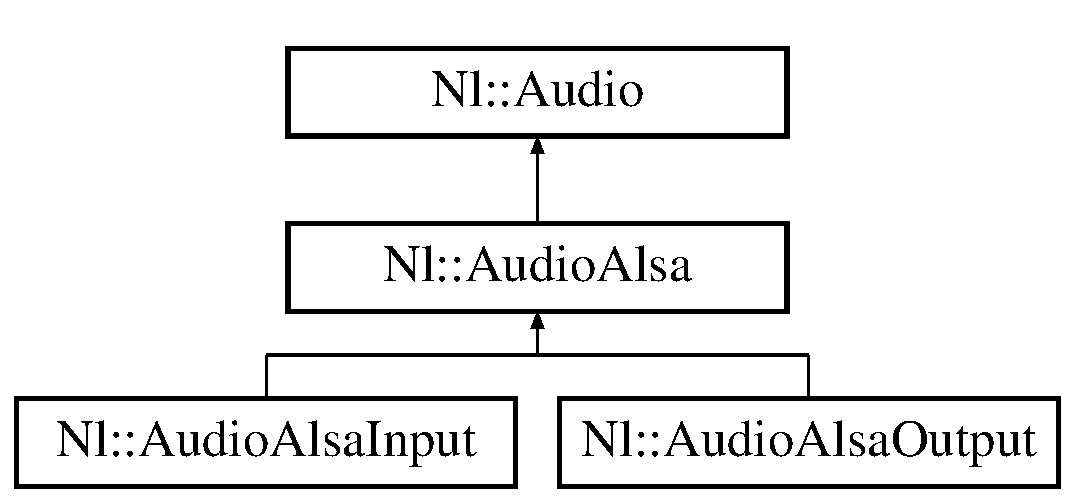
\includegraphics[height=3.000000cm]{classNl_1_1Audio}
\end{center}
\end{figure}
\subsection*{Public Member Functions}
\begin{DoxyCompactItemize}
\item 
\hypertarget{classNl_1_1Audio_a3da276862af02fe20717d07527eb2a3f}{}virtual void {\bfseries open} ()=0\label{classNl_1_1Audio_a3da276862af02fe20717d07527eb2a3f}

\item 
\hypertarget{classNl_1_1Audio_ab8bf0d58ba2f88514c7d6b1756678175}{}virtual void {\bfseries close} ()=0\label{classNl_1_1Audio_ab8bf0d58ba2f88514c7d6b1756678175}

\item 
\hypertarget{classNl_1_1Audio_ad8e03febba94313406f192d7d70eb109}{}virtual void {\bfseries set\+Buffersize} (unsigned int buffersize)=0\label{classNl_1_1Audio_ad8e03febba94313406f192d7d70eb109}

\item 
\hypertarget{classNl_1_1Audio_a2e3c5209b59e9abe5dd7d04dfef301cb}{}virtual unsigned int {\bfseries get\+Buffersize} ()=0\label{classNl_1_1Audio_a2e3c5209b59e9abe5dd7d04dfef301cb}

\item 
\hypertarget{classNl_1_1Audio_a9cca4b557c979fb6bb8c5a7b8978904d}{}virtual void {\bfseries set\+Buffer\+Count} (unsigned int buffercount)=0\label{classNl_1_1Audio_a9cca4b557c979fb6bb8c5a7b8978904d}

\item 
\hypertarget{classNl_1_1Audio_af133dbf0605d95370f745d6d0e7373dc}{}virtual unsigned int {\bfseries get\+Buffer\+Count} ()=0\label{classNl_1_1Audio_af133dbf0605d95370f745d6d0e7373dc}

\item 
\hypertarget{classNl_1_1Audio_a43cd4e1ad7d5b2ff9adc614d31ecd2c8}{}virtual samplerate\+\_\+t {\bfseries get\+Samplerate} () const =0\label{classNl_1_1Audio_a43cd4e1ad7d5b2ff9adc614d31ecd2c8}

\item 
\hypertarget{classNl_1_1Audio_a4aa2440aca1c97e4776c789432f37306}{}virtual void {\bfseries set\+Samplerate} (samplerate\+\_\+t rate)=0\label{classNl_1_1Audio_a4aa2440aca1c97e4776c789432f37306}

\item 
\hypertarget{classNl_1_1Audio_ab75bfef4a7b8cb95fd5e428a9dd2a19f}{}virtual std\+::list$<$ sampleformat\+\_\+t $>$ {\bfseries get\+Available\+Sampleformats} () const =0\label{classNl_1_1Audio_ab75bfef4a7b8cb95fd5e428a9dd2a19f}

\item 
\hypertarget{classNl_1_1Audio_adb6b16848b659bb3e655cd101242f735}{}virtual sampleformat\+\_\+t {\bfseries get\+Sample\+Format} () const =0\label{classNl_1_1Audio_adb6b16848b659bb3e655cd101242f735}

\item 
\hypertarget{classNl_1_1Audio_a60ca413bb266d807fdd99c4aa8bb8881}{}virtual void {\bfseries set\+Sample\+Format} (sampleformat\+\_\+t format)=0\label{classNl_1_1Audio_a60ca413bb266d807fdd99c4aa8bb8881}

\item 
\hypertarget{classNl_1_1Audio_a2c47e7835c7a17389fbfc467d8d5cb72}{}virtual void {\bfseries set\+Channel\+Count} (channelcount\+\_\+t n)=0\label{classNl_1_1Audio_a2c47e7835c7a17389fbfc467d8d5cb72}

\item 
\hypertarget{classNl_1_1Audio_a9acab6c6cdb76c81a3d53e2505ef407a}{}virtual channelcount\+\_\+t {\bfseries get\+Channel\+Count} ()=0\label{classNl_1_1Audio_a9acab6c6cdb76c81a3d53e2505ef407a}

\item 
\hypertarget{classNl_1_1Audio_a7e3523ce7ad5dee987f931f7b68a4581}{}virtual void {\bfseries start} ()=0\label{classNl_1_1Audio_a7e3523ce7ad5dee987f931f7b68a4581}

\item 
\hypertarget{classNl_1_1Audio_af84367ccd7daa7fc6c0bce2d9c7e2b14}{}virtual void {\bfseries stop} ()=0\label{classNl_1_1Audio_af84367ccd7daa7fc6c0bce2d9c7e2b14}

\end{DoxyCompactItemize}


The documentation for this class was generated from the following file\+:\begin{DoxyCompactItemize}
\item 
audio.\+h\end{DoxyCompactItemize}

\hypertarget{classNl_1_1AudioAlsa}{}\section{Nl\+:\+:Audio\+Alsa Class Reference}
\label{classNl_1_1AudioAlsa}\index{Nl\+::\+Audio\+Alsa@{Nl\+::\+Audio\+Alsa}}
Inheritance diagram for Nl\+:\+:Audio\+Alsa\+:\begin{figure}[H]
\begin{center}
\leavevmode
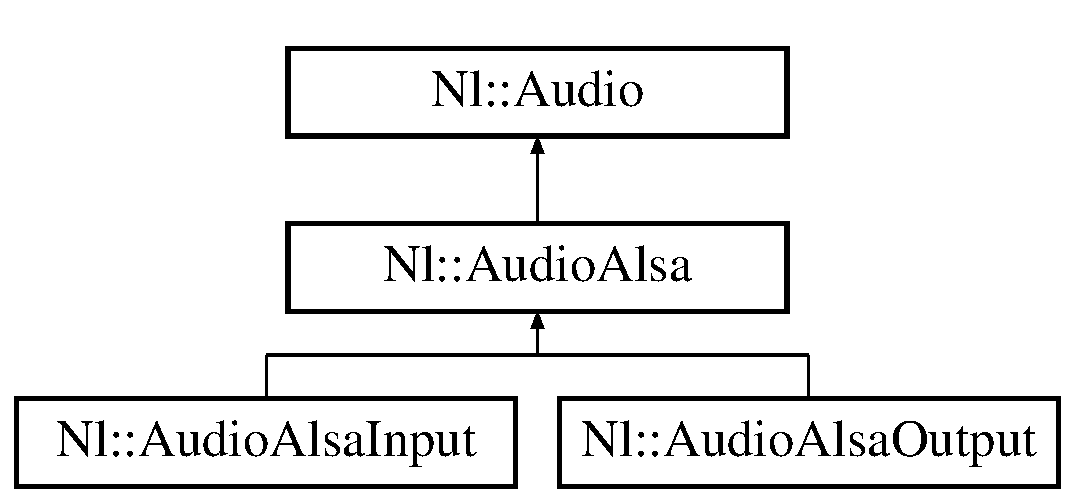
\includegraphics[height=3.000000cm]{classNl_1_1AudioAlsa}
\end{center}
\end{figure}
\subsection*{Public Types}
\begin{DoxyCompactItemize}
\item 
\hypertarget{classNl_1_1AudioAlsa_aad72327bf2bb040c59788d54992510fe}{}typedef \hyperlink{classNl_1_1Audio}{Audio} {\bfseries basetype}\label{classNl_1_1AudioAlsa_aad72327bf2bb040c59788d54992510fe}

\end{DoxyCompactItemize}
\subsection*{Public Member Functions}
\begin{DoxyCompactItemize}
\item 
\hypertarget{classNl_1_1AudioAlsa_a486f9b8b26b8c7eadcc0dec460c1a14a}{}{\bfseries Audio\+Alsa} (const devicename\+\_\+t \&device, std\+::shared\+\_\+ptr$<$ \hyperlink{classNl_1_1BlockingCircularBuffer}{Blocking\+Circular\+Buffer}$<$ u\+\_\+int8\+\_\+t $>$$>$ buffer, bool is\+Input)\label{classNl_1_1AudioAlsa_a486f9b8b26b8c7eadcc0dec460c1a14a}

\item 
\hypertarget{classNl_1_1AudioAlsa_adada0a143dbd23462e3513a467520b8e}{}virtual void {\bfseries open} ()=0\label{classNl_1_1AudioAlsa_adada0a143dbd23462e3513a467520b8e}

\item 
\hypertarget{classNl_1_1AudioAlsa_a99c454b8bb141a18f0ec39955550ca1e}{}virtual void {\bfseries close} ()\label{classNl_1_1AudioAlsa_a99c454b8bb141a18f0ec39955550ca1e}

\item 
\hypertarget{classNl_1_1AudioAlsa_a0c5d5f446b903fb48936c2ebb06b42b9}{}virtual void {\bfseries start} ()=0\label{classNl_1_1AudioAlsa_a0c5d5f446b903fb48936c2ebb06b42b9}

\item 
\hypertarget{classNl_1_1AudioAlsa_a0c02717d31e7e1226dc619b149b631d0}{}virtual void {\bfseries stop} ()=0\label{classNl_1_1AudioAlsa_a0c02717d31e7e1226dc619b149b631d0}

\item 
\hypertarget{classNl_1_1AudioAlsa_aedd7eae90e53aa2fcd3dede15276a7b6}{}virtual void \hyperlink{classNl_1_1AudioAlsa_aedd7eae90e53aa2fcd3dede15276a7b6}{set\+Buffersize} (unsigned int buffersize)\label{classNl_1_1AudioAlsa_aedd7eae90e53aa2fcd3dede15276a7b6}

\begin{DoxyCompactList}\small\item\em Buffersize. \end{DoxyCompactList}\item 
\hypertarget{classNl_1_1AudioAlsa_a61e54f409c8281b3a6dc3feabbe47514}{}virtual unsigned int {\bfseries get\+Buffersize} ()\label{classNl_1_1AudioAlsa_a61e54f409c8281b3a6dc3feabbe47514}

\item 
\hypertarget{classNl_1_1AudioAlsa_a17d24c379eb471145be2e88626e9da6b}{}virtual void \hyperlink{classNl_1_1AudioAlsa_a17d24c379eb471145be2e88626e9da6b}{set\+Buffer\+Count} (unsigned int buffercount)\label{classNl_1_1AudioAlsa_a17d24c379eb471145be2e88626e9da6b}

\begin{DoxyCompactList}\small\item\em Periode Size. \end{DoxyCompactList}\item 
\hypertarget{classNl_1_1AudioAlsa_a17f6570ad5501c84faf0f06ff3378793}{}virtual unsigned int {\bfseries get\+Buffer\+Count} ()\label{classNl_1_1AudioAlsa_a17f6570ad5501c84faf0f06ff3378793}

\item 
\hypertarget{classNl_1_1AudioAlsa_a450390b0bbf9465c0a3c9caaf61a4079}{}virtual samplerate\+\_\+t \hyperlink{classNl_1_1AudioAlsa_a450390b0bbf9465c0a3c9caaf61a4079}{get\+Samplerate} () const \label{classNl_1_1AudioAlsa_a450390b0bbf9465c0a3c9caaf61a4079}

\begin{DoxyCompactList}\small\item\em Sample Rate. \end{DoxyCompactList}\item 
\hypertarget{classNl_1_1AudioAlsa_a892cf5818d0e7fa43ebc85f4d882f804}{}virtual void {\bfseries set\+Samplerate} (samplerate\+\_\+t rate)\label{classNl_1_1AudioAlsa_a892cf5818d0e7fa43ebc85f4d882f804}

\item 
\hypertarget{classNl_1_1AudioAlsa_a5c95174097753e5bae87e3f943b042c9}{}virtual std\+::list$<$ sampleformat\+\_\+t $>$ \hyperlink{classNl_1_1AudioAlsa_a5c95174097753e5bae87e3f943b042c9}{get\+Available\+Sampleformats} () const \label{classNl_1_1AudioAlsa_a5c95174097753e5bae87e3f943b042c9}

\begin{DoxyCompactList}\small\item\em Sample Format. \end{DoxyCompactList}\item 
\hypertarget{classNl_1_1AudioAlsa_accc91631cf20bc1de1add888c30e007e}{}virtual sampleformat\+\_\+t {\bfseries get\+Sample\+Format} () const \label{classNl_1_1AudioAlsa_accc91631cf20bc1de1add888c30e007e}

\item 
\hypertarget{classNl_1_1AudioAlsa_adfd02364854decfdae10f1dcfcf5292d}{}virtual void {\bfseries set\+Sample\+Format} (sampleformat\+\_\+t format)\label{classNl_1_1AudioAlsa_adfd02364854decfdae10f1dcfcf5292d}

\item 
\hypertarget{classNl_1_1AudioAlsa_aad4859e60c5b2f393224d9fe8728bd74}{}virtual void \hyperlink{classNl_1_1AudioAlsa_aad4859e60c5b2f393224d9fe8728bd74}{set\+Channel\+Count} (channelcount\+\_\+t n)\label{classNl_1_1AudioAlsa_aad4859e60c5b2f393224d9fe8728bd74}

\begin{DoxyCompactList}\small\item\em Channels. \end{DoxyCompactList}\item 
\hypertarget{classNl_1_1AudioAlsa_aad8e4064dc35ecba3e0ce74a7d10e8a8}{}virtual channelcount\+\_\+t {\bfseries get\+Channel\+Count} ()\label{classNl_1_1AudioAlsa_aad8e4064dc35ecba3e0ce74a7d10e8a8}

\item 
\hypertarget{classNl_1_1AudioAlsa_a9da16275704c5646db14b94dd02ca3e6}{}\hyperlink{structNl_1_1Statistics}{Statistics} {\bfseries get\+Stats} ()\label{classNl_1_1AudioAlsa_a9da16275704c5646db14b94dd02ca3e6}

\end{DoxyCompactItemize}
\subsection*{Static Public Member Functions}
\begin{DoxyCompactItemize}
\item 
\hypertarget{classNl_1_1AudioAlsa_a6c1969f1f344b8a13c27e26e02279c54}{}static std\+::list$<$ \hyperlink{classNl_1_1AlsaDeviceIdentifier}{Alsa\+Device\+Identifier} $>$ \hyperlink{classNl_1_1AudioAlsa_a6c1969f1f344b8a13c27e26e02279c54}{get\+Available\+Devices} ()\label{classNl_1_1AudioAlsa_a6c1969f1f344b8a13c27e26e02279c54}

\begin{DoxyCompactList}\small\item\em Static. \end{DoxyCompactList}\end{DoxyCompactItemize}
\subsection*{Protected Member Functions}
\begin{DoxyCompactItemize}
\item 
\hypertarget{classNl_1_1AudioAlsa_a412c7a2b30dfb3b1b49ce63b7e84eb52}{}void \hyperlink{classNl_1_1AudioAlsa_a412c7a2b30dfb3b1b49ce63b7e84eb52}{open\+Common} ()\label{classNl_1_1AudioAlsa_a412c7a2b30dfb3b1b49ce63b7e84eb52}

\begin{DoxyCompactList}\small\item\em Open / Close. \end{DoxyCompactList}\item 
\hypertarget{classNl_1_1AudioAlsa_a409e810baf7f4c3f1ff7380b1f979721}{}void {\bfseries throw\+On\+Device\+Closed} (const std\+::string \&file, const std\+::string \&func, int line) const \label{classNl_1_1AudioAlsa_a409e810baf7f4c3f1ff7380b1f979721}

\item 
\hypertarget{classNl_1_1AudioAlsa_a96f03f2ab93bf0caec1ca9dc9fc03d6b}{}void {\bfseries throw\+On\+Device\+Running} (const std\+::string \&file, const std\+::string \&func, int line) const \label{classNl_1_1AudioAlsa_a96f03f2ab93bf0caec1ca9dc9fc03d6b}

\item 
\hypertarget{classNl_1_1AudioAlsa_af19fdd267bd17b21c0961cf6c17038c1}{}void {\bfseries set\+Terminate\+Request} ()\label{classNl_1_1AudioAlsa_af19fdd267bd17b21c0961cf6c17038c1}

\item 
\hypertarget{classNl_1_1AudioAlsa_aad8b3bce72a0812a4878d007006cd767}{}void {\bfseries reset\+Terminate\+Request} ()\label{classNl_1_1AudioAlsa_aad8b3bce72a0812a4878d007006cd767}

\item 
\hypertarget{classNl_1_1AudioAlsa_ac59db37cfc168cca3cad339b73798f6a}{}bool {\bfseries get\+Terminate\+Request} () const \label{classNl_1_1AudioAlsa_ac59db37cfc168cca3cad339b73798f6a}

\item 
\hypertarget{classNl_1_1AudioAlsa_acff797a11843617d06870f1fdef8fd2e}{}\hyperlink{structNl_1_1SampleSpecs__t}{Sample\+Specs\+\_\+t} \hyperlink{classNl_1_1AudioAlsa_acff797a11843617d06870f1fdef8fd2e}{get\+Specs} ()\label{classNl_1_1AudioAlsa_acff797a11843617d06870f1fdef8fd2e}

\begin{DoxyCompactList}\small\item\em Sample\+Specs. \end{DoxyCompactList}\item 
\hypertarget{classNl_1_1AudioAlsa_a49001b5030e29d798858025458a0d8ad}{}void {\bfseries throw\+On\+Alsa\+Error} (const std\+::string \&file, const std\+::string \&func, int line, int e) const \label{classNl_1_1AudioAlsa_a49001b5030e29d798858025458a0d8ad}

\end{DoxyCompactItemize}
\subsection*{Static Protected Member Functions}
\begin{DoxyCompactItemize}
\item 
\hypertarget{classNl_1_1AudioAlsa_a3bfd0415c0694893adda600459e54d2e}{}static int \hyperlink{classNl_1_1AudioAlsa_a3bfd0415c0694893adda600459e54d2e}{xrun\+Recovery} (\hyperlink{classNl_1_1AudioAlsa}{Audio\+Alsa} $\ast$ptr, int err)\label{classNl_1_1AudioAlsa_a3bfd0415c0694893adda600459e54d2e}

\begin{DoxyCompactList}\small\item\em Static. \end{DoxyCompactList}\end{DoxyCompactItemize}
\subsection*{Protected Attributes}
\begin{DoxyCompactItemize}
\item 
\hypertarget{classNl_1_1AudioAlsa_a70f80e5c44e951342e09d068ab85c7ba}{}snd\+\_\+pcm\+\_\+t $\ast$ {\bfseries m\+\_\+handle}\label{classNl_1_1AudioAlsa_a70f80e5c44e951342e09d068ab85c7ba}

\item 
\hypertarget{classNl_1_1AudioAlsa_ad42539868b85e4ff8a4b16871023df19}{}std\+::thread $\ast$ {\bfseries m\+\_\+audio\+Thread}\label{classNl_1_1AudioAlsa_ad42539868b85e4ff8a4b16871023df19}

\item 
\hypertarget{classNl_1_1AudioAlsa_a7511d35af0abe3d73b79c0e620a625cc}{}snd\+\_\+pcm\+\_\+hw\+\_\+params\+\_\+t $\ast$ {\bfseries m\+\_\+hw\+Params}\label{classNl_1_1AudioAlsa_a7511d35af0abe3d73b79c0e620a625cc}

\item 
\hypertarget{classNl_1_1AudioAlsa_aaa68b97a4c444118d668ef670047ba0f}{}std\+::atomic$<$ bool $>$ {\bfseries m\+\_\+request\+Terminate}\label{classNl_1_1AudioAlsa_aaa68b97a4c444118d668ef670047ba0f}

\item 
\hypertarget{classNl_1_1AudioAlsa_abdc14902d5b5b53baa2842e1a37cfc46}{}std\+::atomic$<$ unsigned int $>$ {\bfseries m\+\_\+xrun\+Recovery\+Counter}\label{classNl_1_1AudioAlsa_abdc14902d5b5b53baa2842e1a37cfc46}

\item 
\hypertarget{classNl_1_1AudioAlsa_adff181d43b67dbda1821144371c36526}{}std\+::shared\+\_\+ptr$<$ \hyperlink{classNl_1_1BlockingCircularBuffer}{Blocking\+Circular\+Buffer}$<$ u\+\_\+int8\+\_\+t $>$ $>$ {\bfseries m\+\_\+audio\+Buffer}\label{classNl_1_1AudioAlsa_adff181d43b67dbda1821144371c36526}

\end{DoxyCompactItemize}


The documentation for this class was generated from the following files\+:\begin{DoxyCompactItemize}
\item 
audioalsa.\+h\item 
audioalsa.\+cpp\end{DoxyCompactItemize}

\hypertarget{classNl_1_1AudioAlsaException}{}\section{Nl\+:\+:Audio\+Alsa\+Exception Class Reference}
\label{classNl_1_1AudioAlsaException}\index{Nl\+::\+Audio\+Alsa\+Exception@{Nl\+::\+Audio\+Alsa\+Exception}}
Inheritance diagram for Nl\+:\+:Audio\+Alsa\+Exception\+:\begin{figure}[H]
\begin{center}
\leavevmode
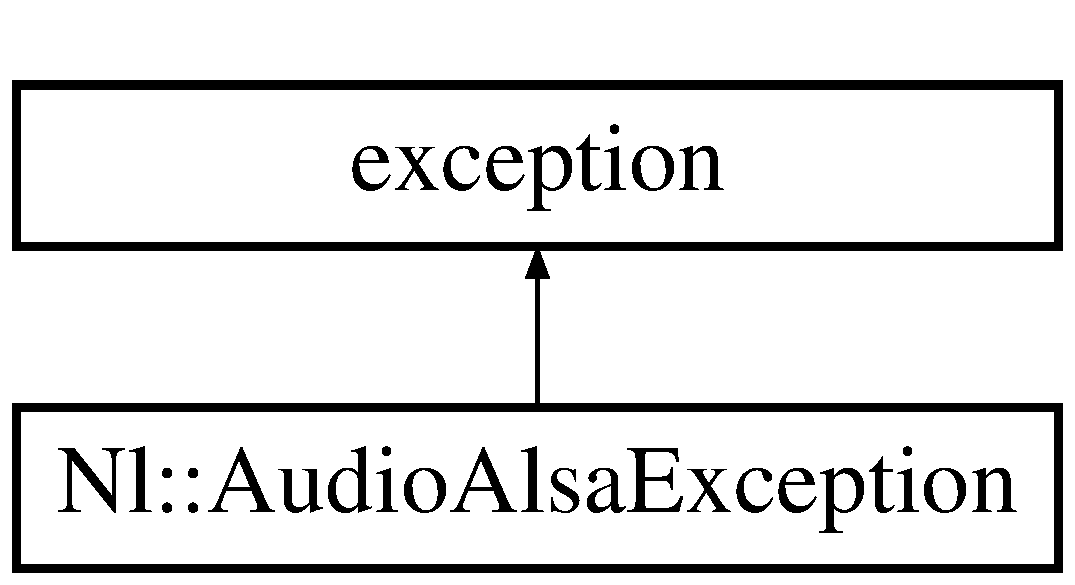
\includegraphics[height=2.000000cm]{classNl_1_1AudioAlsaException}
\end{center}
\end{figure}
\subsection*{Public Member Functions}
\begin{DoxyCompactItemize}
\item 
\hypertarget{classNl_1_1AudioAlsaException_a6c40dfc626db2587fc521cd9778fbc24}{}{\bfseries Audio\+Alsa\+Exception} (std\+::string func, std\+::string file, int line, int error\+Number, std\+::string what)\label{classNl_1_1AudioAlsaException_a6c40dfc626db2587fc521cd9778fbc24}

\item 
\hypertarget{classNl_1_1AudioAlsaException_a3fdf23855f8f24b2123782564d48bfb7}{}virtual const char $\ast$ {\bfseries what} () const noexcept\label{classNl_1_1AudioAlsaException_a3fdf23855f8f24b2123782564d48bfb7}

\end{DoxyCompactItemize}


The documentation for this class was generated from the following file\+:\begin{DoxyCompactItemize}
\item 
audioalsa.\+h\end{DoxyCompactItemize}

\hypertarget{classNl_1_1AudioAlsaInput}{\section{Nl\-:\-:Audio\-Alsa\-Input Class Reference}
\label{classNl_1_1AudioAlsaInput}\index{Nl\-::\-Audio\-Alsa\-Input@{Nl\-::\-Audio\-Alsa\-Input}}
}
Inheritance diagram for Nl\-:\-:Audio\-Alsa\-Input\-:\begin{figure}[H]
\begin{center}
\leavevmode
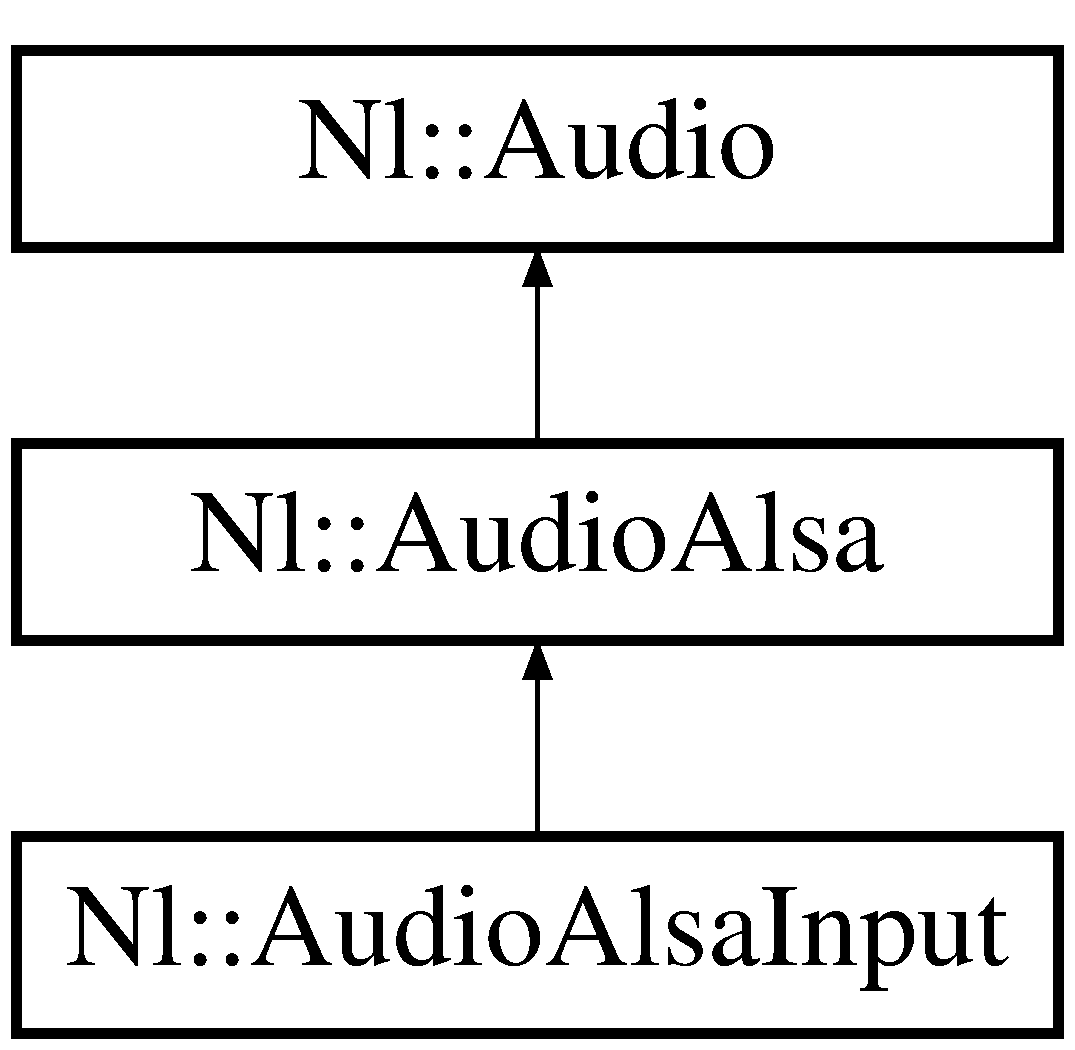
\includegraphics[height=3.000000cm]{classNl_1_1AudioAlsaInput}
\end{center}
\end{figure}
\subsection*{Public Types}
\begin{DoxyCompactItemize}
\item 
\hypertarget{classNl_1_1AudioAlsaInput_ac39e7e54c4aaaaa5c294c95cda6e3d87}{typedef \hyperlink{classNl_1_1AudioAlsa}{Audio\-Alsa} {\bfseries basetype}}\label{classNl_1_1AudioAlsaInput_ac39e7e54c4aaaaa5c294c95cda6e3d87}

\end{DoxyCompactItemize}
\subsection*{Public Member Functions}
\begin{DoxyCompactItemize}
\item 
\hypertarget{classNl_1_1AudioAlsaInput_ac2d6401ab9becd5f88a9a6484f2f9257}{{\bfseries Audio\-Alsa\-Input} (const \hyperlink{classNl_1_1AlsaCardIdentifier}{Alsa\-Card\-Identifier} \&card, Shared\-Buffer\-Handle buffer)}\label{classNl_1_1AudioAlsaInput_ac2d6401ab9becd5f88a9a6484f2f9257}

\item 
virtual void \hyperlink{classNl_1_1AudioAlsaInput_a9e3afb8dfb0615d745a4f362302ce99d}{open} ()
\begin{DoxyCompactList}\small\item\em Open the audio device. \end{DoxyCompactList}\item 
virtual void \hyperlink{classNl_1_1AudioAlsaInput_a9b8aa604c6e78b93b337ae68cb071e00}{start} ()
\begin{DoxyCompactList}\small\item\em Starts the working thread for the interface. \end{DoxyCompactList}\item 
virtual void \hyperlink{classNl_1_1AudioAlsaInput_a728ce3af74d71e387834a28922fc98c1}{stop} ()
\begin{DoxyCompactList}\small\item\em Stopps the working thread for the interface. \end{DoxyCompactList}\end{DoxyCompactItemize}
\subsection*{Static Public Member Functions}
\begin{DoxyCompactItemize}
\item 
\hypertarget{classNl_1_1AudioAlsaInput_abc2e1cd6bf4f23627565a127ac708fe1}{static void {\bfseries worker} (\hyperlink{structNl_1_1SampleSpecs}{Sample\-Specs} specs, \hyperlink{classNl_1_1AudioAlsaInput}{Audio\-Alsa\-Input} $\ast$ptr)}\label{classNl_1_1AudioAlsaInput_abc2e1cd6bf4f23627565a127ac708fe1}

\end{DoxyCompactItemize}
\subsection*{Additional Inherited Members}


\subsection{Member Function Documentation}
\hypertarget{classNl_1_1AudioAlsaInput_a9e3afb8dfb0615d745a4f362302ce99d}{\index{Nl\-::\-Audio\-Alsa\-Input@{Nl\-::\-Audio\-Alsa\-Input}!open@{open}}
\index{open@{open}!Nl::AudioAlsaInput@{Nl\-::\-Audio\-Alsa\-Input}}
\subsubsection[{open}]{\setlength{\rightskip}{0pt plus 5cm}void Nl\-::\-Audio\-Alsa\-Input\-::open (
\begin{DoxyParamCaption}
{}
\end{DoxyParamCaption}
)\hspace{0.3cm}{\ttfamily [virtual]}}}\label{classNl_1_1AudioAlsaInput_a9e3afb8dfb0615d745a4f362302ce99d}


Open the audio device. 


\begin{DoxyExceptions}{Exceptions}
{\em \hyperlink{classNl_1_1AudioAlsaException}{Audio\-Alsa\-Exception}} & is thrown on error\\
\hline
\end{DoxyExceptions}
Opens the audio device, represented by that class. On error a \hyperlink{classNl_1_1AudioAlsaException}{Audio\-Alsa\-Exception} is thrown. 

Implements \hyperlink{classNl_1_1AudioAlsa_adada0a143dbd23462e3513a467520b8e}{Nl\-::\-Audio\-Alsa}.

\hypertarget{classNl_1_1AudioAlsaInput_a9b8aa604c6e78b93b337ae68cb071e00}{\index{Nl\-::\-Audio\-Alsa\-Input@{Nl\-::\-Audio\-Alsa\-Input}!start@{start}}
\index{start@{start}!Nl::AudioAlsaInput@{Nl\-::\-Audio\-Alsa\-Input}}
\subsubsection[{start}]{\setlength{\rightskip}{0pt plus 5cm}void Nl\-::\-Audio\-Alsa\-Input\-::start (
\begin{DoxyParamCaption}
{}
\end{DoxyParamCaption}
)\hspace{0.3cm}{\ttfamily [virtual]}}}\label{classNl_1_1AudioAlsaInput_a9b8aa604c6e78b93b337ae68cb071e00}


Starts the working thread for the interface. 


\begin{DoxyExceptions}{Exceptions}
{\em \hyperlink{classNl_1_1AudioAlsaException}{Audio\-Alsa\-Exception}} & is thrown on error\\
\hline
\end{DoxyExceptions}
Returns the number of channels. On error a \hyperlink{classNl_1_1AudioAlsaException}{Audio\-Alsa\-Exception} is thrown. 

Implements \hyperlink{classNl_1_1AudioAlsa_a0c5d5f446b903fb48936c2ebb06b42b9}{Nl\-::\-Audio\-Alsa}.

\hypertarget{classNl_1_1AudioAlsaInput_a728ce3af74d71e387834a28922fc98c1}{\index{Nl\-::\-Audio\-Alsa\-Input@{Nl\-::\-Audio\-Alsa\-Input}!stop@{stop}}
\index{stop@{stop}!Nl::AudioAlsaInput@{Nl\-::\-Audio\-Alsa\-Input}}
\subsubsection[{stop}]{\setlength{\rightskip}{0pt plus 5cm}void Nl\-::\-Audio\-Alsa\-Input\-::stop (
\begin{DoxyParamCaption}
{}
\end{DoxyParamCaption}
)\hspace{0.3cm}{\ttfamily [virtual]}}}\label{classNl_1_1AudioAlsaInput_a728ce3af74d71e387834a28922fc98c1}


Stopps the working thread for the interface. 


\begin{DoxyExceptions}{Exceptions}
{\em \hyperlink{classNl_1_1AudioAlsaException}{Audio\-Alsa\-Exception}} & is thrown on error\\
\hline
\end{DoxyExceptions}
Returns the number of channels. On error a \hyperlink{classNl_1_1AudioAlsaException}{Audio\-Alsa\-Exception} is thrown. 

Implements \hyperlink{classNl_1_1AudioAlsa_a0c02717d31e7e1226dc619b149b631d0}{Nl\-::\-Audio\-Alsa}.



The documentation for this class was generated from the following files\-:\begin{DoxyCompactItemize}
\item 
audioalsainput.\-h\item 
audioalsainput.\-cpp\end{DoxyCompactItemize}

\hypertarget{classNl_1_1AudioAlsaOutput}{\section{Nl\-:\-:Audio\-Alsa\-Output Class Reference}
\label{classNl_1_1AudioAlsaOutput}\index{Nl\-::\-Audio\-Alsa\-Output@{Nl\-::\-Audio\-Alsa\-Output}}
}
Inheritance diagram for Nl\-:\-:Audio\-Alsa\-Output\-:\begin{figure}[H]
\begin{center}
\leavevmode
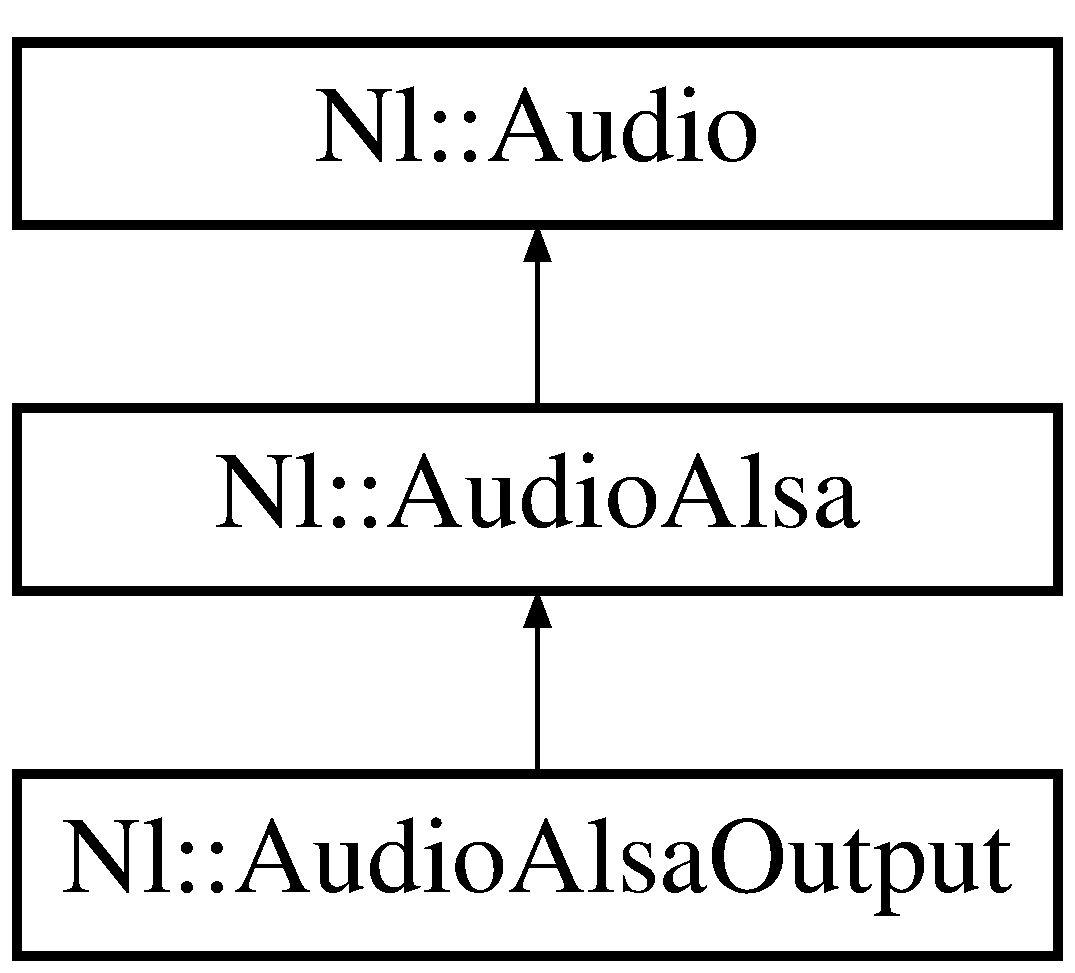
\includegraphics[height=3.000000cm]{classNl_1_1AudioAlsaOutput}
\end{center}
\end{figure}
\subsection*{Public Types}
\begin{DoxyCompactItemize}
\item 
\hypertarget{classNl_1_1AudioAlsaOutput_abd57cd3efbb62397d017dc0eff54da3e}{typedef \hyperlink{classNl_1_1AudioAlsa}{Audio\-Alsa} {\bfseries basetype}}\label{classNl_1_1AudioAlsaOutput_abd57cd3efbb62397d017dc0eff54da3e}

\end{DoxyCompactItemize}
\subsection*{Public Member Functions}
\begin{DoxyCompactItemize}
\item 
\hypertarget{classNl_1_1AudioAlsaOutput_a27bd852a0c3459500ad2b28317fe3e9d}{{\bfseries Audio\-Alsa\-Output} (const \hyperlink{classNl_1_1AlsaCardIdentifier}{Alsa\-Card\-Identifier} \&card, Shared\-Buffer\-Handle buffer)}\label{classNl_1_1AudioAlsaOutput_a27bd852a0c3459500ad2b28317fe3e9d}

\item 
virtual void \hyperlink{classNl_1_1AudioAlsaOutput_a94792430810853353314a71f1b54a5d3}{open} ()
\begin{DoxyCompactList}\small\item\em Open the audio device. \end{DoxyCompactList}\item 
virtual void \hyperlink{classNl_1_1AudioAlsaOutput_a9d2239af344a6773942add0dc38514d3}{start} ()
\begin{DoxyCompactList}\small\item\em Starts the working thread for the interface. \end{DoxyCompactList}\item 
virtual void \hyperlink{classNl_1_1AudioAlsaOutput_acd8cb8bfe0722c1c20d8da0f3963683e}{stop} ()
\begin{DoxyCompactList}\small\item\em Stopps the working thread for the interface. \end{DoxyCompactList}\end{DoxyCompactItemize}
\subsection*{Static Public Member Functions}
\begin{DoxyCompactItemize}
\item 
\hypertarget{classNl_1_1AudioAlsaOutput_acae749e941cb4a053494e7233e90cfdc}{static void {\bfseries worker} (\hyperlink{structNl_1_1SampleSpecs}{Sample\-Specs} specs, \hyperlink{classNl_1_1AudioAlsaOutput}{Audio\-Alsa\-Output} $\ast$ptr)}\label{classNl_1_1AudioAlsaOutput_acae749e941cb4a053494e7233e90cfdc}

\end{DoxyCompactItemize}
\subsection*{Additional Inherited Members}


\subsection{Member Function Documentation}
\hypertarget{classNl_1_1AudioAlsaOutput_a94792430810853353314a71f1b54a5d3}{\index{Nl\-::\-Audio\-Alsa\-Output@{Nl\-::\-Audio\-Alsa\-Output}!open@{open}}
\index{open@{open}!Nl::AudioAlsaOutput@{Nl\-::\-Audio\-Alsa\-Output}}
\subsubsection[{open}]{\setlength{\rightskip}{0pt plus 5cm}void Nl\-::\-Audio\-Alsa\-Output\-::open (
\begin{DoxyParamCaption}
{}
\end{DoxyParamCaption}
)\hspace{0.3cm}{\ttfamily [virtual]}}}\label{classNl_1_1AudioAlsaOutput_a94792430810853353314a71f1b54a5d3}


Open the audio device. 


\begin{DoxyExceptions}{Exceptions}
{\em \hyperlink{classNl_1_1AudioAlsaException}{Audio\-Alsa\-Exception}} & is thrown on error\\
\hline
\end{DoxyExceptions}
Opens the audio device, represented by that class. On error a \hyperlink{classNl_1_1AudioAlsaException}{Audio\-Alsa\-Exception} is thrown. 

Implements \hyperlink{classNl_1_1AudioAlsa_adada0a143dbd23462e3513a467520b8e}{Nl\-::\-Audio\-Alsa}.

\hypertarget{classNl_1_1AudioAlsaOutput_a9d2239af344a6773942add0dc38514d3}{\index{Nl\-::\-Audio\-Alsa\-Output@{Nl\-::\-Audio\-Alsa\-Output}!start@{start}}
\index{start@{start}!Nl::AudioAlsaOutput@{Nl\-::\-Audio\-Alsa\-Output}}
\subsubsection[{start}]{\setlength{\rightskip}{0pt plus 5cm}void Nl\-::\-Audio\-Alsa\-Output\-::start (
\begin{DoxyParamCaption}
{}
\end{DoxyParamCaption}
)\hspace{0.3cm}{\ttfamily [virtual]}}}\label{classNl_1_1AudioAlsaOutput_a9d2239af344a6773942add0dc38514d3}


Starts the working thread for the interface. 


\begin{DoxyExceptions}{Exceptions}
{\em \hyperlink{classNl_1_1AudioAlsaException}{Audio\-Alsa\-Exception}} & is thrown on error\\
\hline
\end{DoxyExceptions}
Returns the number of channels. On error a \hyperlink{classNl_1_1AudioAlsaException}{Audio\-Alsa\-Exception} is thrown. 

Implements \hyperlink{classNl_1_1AudioAlsa_a0c5d5f446b903fb48936c2ebb06b42b9}{Nl\-::\-Audio\-Alsa}.

\hypertarget{classNl_1_1AudioAlsaOutput_acd8cb8bfe0722c1c20d8da0f3963683e}{\index{Nl\-::\-Audio\-Alsa\-Output@{Nl\-::\-Audio\-Alsa\-Output}!stop@{stop}}
\index{stop@{stop}!Nl::AudioAlsaOutput@{Nl\-::\-Audio\-Alsa\-Output}}
\subsubsection[{stop}]{\setlength{\rightskip}{0pt plus 5cm}void Nl\-::\-Audio\-Alsa\-Output\-::stop (
\begin{DoxyParamCaption}
{}
\end{DoxyParamCaption}
)\hspace{0.3cm}{\ttfamily [virtual]}}}\label{classNl_1_1AudioAlsaOutput_acd8cb8bfe0722c1c20d8da0f3963683e}


Stopps the working thread for the interface. 


\begin{DoxyExceptions}{Exceptions}
{\em \hyperlink{classNl_1_1AudioAlsaException}{Audio\-Alsa\-Exception}} & is thrown on error\\
\hline
\end{DoxyExceptions}
Returns the number of channels. On error a \hyperlink{classNl_1_1AudioAlsaException}{Audio\-Alsa\-Exception} is thrown. 

Implements \hyperlink{classNl_1_1AudioAlsa_a0c02717d31e7e1226dc619b149b631d0}{Nl\-::\-Audio\-Alsa}.



The documentation for this class was generated from the following files\-:\begin{DoxyCompactItemize}
\item 
audioalsaoutput.\-h\item 
audioalsaoutput.\-cpp\end{DoxyCompactItemize}

\hypertarget{classNl_1_1BlockingCircularBuffer}{\section{Nl\-:\-:Blocking\-Circular\-Buffer$<$ T $>$ Class Template Reference}
\label{classNl_1_1BlockingCircularBuffer}\index{Nl\-::\-Blocking\-Circular\-Buffer$<$ T $>$@{Nl\-::\-Blocking\-Circular\-Buffer$<$ T $>$}}
}


A blocking circular buffer implementation.  




{\ttfamily \#include $<$blockingcircularbuffer.\-h$>$}

\subsection*{Public Member Functions}
\begin{DoxyCompactItemize}
\item 
\hyperlink{group__Audio_gaff1f3f4ae609326ed19b4764a7516c32}{Blocking\-Circular\-Buffer} (const std\-::string \&\hyperlink{group__Audio_gad287c03d36b07643b960d531b5553109}{name})
\begin{DoxyCompactList}\small\item\em Constructor. \end{DoxyCompactList}\item 
\hypertarget{classNl_1_1BlockingCircularBuffer_a85819f06c4bf4962b4cd85ac4c675ae2}{void {\bfseries init} (int \hyperlink{group__Audio_ga8e5076598374af82eb754cea0c88d12d}{size})}\label{classNl_1_1BlockingCircularBuffer_a85819f06c4bf4962b4cd85ac4c675ae2}

\item 
\hypertarget{classNl_1_1BlockingCircularBuffer_a43aac3ecb00a1e96ae7cbd615db69327}{void {\bfseries init} (const \hyperlink{structNl_1_1SampleSpecs}{Sample\-Specs} \&\hyperlink{group__Audio_ga679616fc01beaa6db6774a5cdabc5cd9}{sample\-Specs})}\label{classNl_1_1BlockingCircularBuffer_a43aac3ecb00a1e96ae7cbd615db69327}

\item 
void \hyperlink{group__Audio_ga3923df13e2115ece2a5f4969a9b2f890}{get} (T $\ast$buffer, unsigned int \hyperlink{group__Audio_ga8e5076598374af82eb754cea0c88d12d}{size})
\begin{DoxyCompactList}\small\item\em Read data from the buffer. \end{DoxyCompactList}\item 
void \hyperlink{group__Audio_gab60ad480d2ebe4b2aa526d31d808be7a}{set} (T $\ast$buffer, unsigned int \hyperlink{group__Audio_ga8e5076598374af82eb754cea0c88d12d}{size})
\begin{DoxyCompactList}\small\item\em Write data to the buffer. \end{DoxyCompactList}\item 
void \hyperlink{group__Audio_ga012421a899e2da4cf994556ccfcb1880}{get\-Stat} (unsigned long $\ast$read\-Bytes, unsigned long $\ast$written\-Bytes) const 
\begin{DoxyCompactList}\small\item\em Returns information on read/write cycles on the buffer. \end{DoxyCompactList}\item 
unsigned int \hyperlink{group__Audio_ga75e3bbb71d5eeb19224f1503d58e1b0a}{available\-To\-Read} () const 
\begin{DoxyCompactList}\small\item\em Returns number of available elements to read. \end{DoxyCompactList}\item 
unsigned int \hyperlink{group__Audio_ga440f66059781b20486d6d6c160e4f0ed}{available\-To\-Write} () const 
\begin{DoxyCompactList}\small\item\em Returns number of available elements to write. \end{DoxyCompactList}\item 
int \hyperlink{group__Audio_ga8e5076598374af82eb754cea0c88d12d}{size} () const 
\begin{DoxyCompactList}\small\item\em Returns the size of the buffer in elements. \end{DoxyCompactList}\item 
std\-::string \hyperlink{group__Audio_gad287c03d36b07643b960d531b5553109}{name} () const 
\begin{DoxyCompactList}\small\item\em Returns the name of the buffer. \end{DoxyCompactList}\item 
\hyperlink{structNl_1_1SampleSpecs}{Sample\-Specs} \hyperlink{group__Audio_ga679616fc01beaa6db6774a5cdabc5cd9}{sample\-Specs} ()
\begin{DoxyCompactList}\small\item\em Returns the Sample\-Specs\-\_\-t of the buffer. \end{DoxyCompactList}\end{DoxyCompactItemize}


\subsection{Detailed Description}
\subsubsection*{template$<$typename T$>$class Nl\-::\-Blocking\-Circular\-Buffer$<$ T $>$}

A blocking circular buffer implementation. 


\begin{DoxyTemplParams}{Template Parameters}
{\em Type} & of buffer elements \\
\hline
\end{DoxyTemplParams}

\begin{DoxyParams}{Parameters}
{\em size} & Buffersize in elements of type T\\
\hline
\end{DoxyParams}
A circular buffer implementation which blocks the callee of \hyperlink{group__Audio_ga3923df13e2115ece2a5f4969a9b2f890}{get()} if nothing to read and the callee of \hyperlink{group__Audio_gab60ad480d2ebe4b2aa526d31d808be7a}{set()} when no space to write 

The documentation for this class was generated from the following file\-:\begin{DoxyCompactItemize}
\item 
blockingcircularbuffer.\-h\end{DoxyCompactItemize}

\hypertarget{classNl_1_1BlockingLinearBuffer}{}\section{Nl\+:\+:Blocking\+Linear\+Buffer$<$ T $>$ Class Template Reference}
\label{classNl_1_1BlockingLinearBuffer}\index{Nl\+::\+Blocking\+Linear\+Buffer$<$ T $>$@{Nl\+::\+Blocking\+Linear\+Buffer$<$ T $>$}}


A blocking linear buffer implementation.  




{\ttfamily \#include $<$blockinglinearbuffer.\+h$>$}

\subsection*{Public Member Functions}
\begin{DoxyCompactItemize}
\item 
\hyperlink{group__Audio_gae6f35f45439b194a69587bd9c124a736}{Blocking\+Linear\+Buffer} (unsigned int size)
\begin{DoxyCompactList}\small\item\em Constructor. \end{DoxyCompactList}\item 
void \hyperlink{group__Audio_ga7fd45f57444309f03fab9a13644d2240}{Blocking\+Linear\+Buffer\+::get} (T $\ast$buffer, unsigned int size)
\begin{DoxyCompactList}\small\item\em Read data from the buffer. \end{DoxyCompactList}\item 
void \hyperlink{group__Audio_gacd7c49cb333fc991edae3247d2fb34ef}{set} (void $\ast$buffer, unsigned int size)
\begin{DoxyCompactList}\small\item\em Write data to the buffer. \end{DoxyCompactList}\item 
\hyperlink{group__Audio_gabdd2b325cd5a2383579737299b4b3aca}{get\+Stat} (unsigned long $\ast$read\+Bytes, unsigned long $\ast$written\+Bytes)
\begin{DoxyCompactList}\small\item\em Returns information on read/write cycles on the buffer. \end{DoxyCompactList}\end{DoxyCompactItemize}


\subsection{Detailed Description}
\subsubsection*{template$<$typename T$>$class Nl\+::\+Blocking\+Linear\+Buffer$<$ T $>$}

A blocking linear buffer implementation. 


\begin{DoxyTemplParams}{Template Parameters}
{\em Type} & of buffer elements \\
\hline
\end{DoxyTemplParams}

\begin{DoxyParams}{Parameters}
{\em size} & Buffersize in elements of type T\\
\hline
\end{DoxyParams}
A linear buffer implementation which blocks the callee of get() if nothing to read and the callee of \hyperlink{group__Audio_gacd7c49cb333fc991edae3247d2fb34ef}{set()} if no space to write 

The documentation for this class was generated from the following file\+:\begin{DoxyCompactItemize}
\item 
blockinglinearbuffer.\+h\end{DoxyCompactItemize}

\hypertarget{structNl_1_1BufferStatistics}{\section{Nl\-:\-:Buffer\-Statistics Struct Reference}
\label{structNl_1_1BufferStatistics}\index{Nl\-::\-Buffer\-Statistics@{Nl\-::\-Buffer\-Statistics}}
}
\subsection*{Data Fields}
\begin{DoxyCompactItemize}
\item 
\hypertarget{structNl_1_1BufferStatistics_a54af55bf586df1a2c2e650f03b00692b}{unsigned long \hyperlink{structNl_1_1BufferStatistics_a54af55bf586df1a2c2e650f03b00692b}{bytes\-Read\-From\-Buffer}}\label{structNl_1_1BufferStatistics_a54af55bf586df1a2c2e650f03b00692b}

\begin{DoxyCompactList}\small\item\em Number of bytes that have been read from the buffer. \end{DoxyCompactList}\item 
\hypertarget{structNl_1_1BufferStatistics_aa3b2e11bb9ca059ee93feb45ea63b1b4}{unsigned long \hyperlink{structNl_1_1BufferStatistics_aa3b2e11bb9ca059ee93feb45ea63b1b4}{bytes\-Written\-To\-Buffer}}\label{structNl_1_1BufferStatistics_aa3b2e11bb9ca059ee93feb45ea63b1b4}

\begin{DoxyCompactList}\small\item\em Number of bytes that have been written to the buffer. \end{DoxyCompactList}\item 
\hypertarget{structNl_1_1BufferStatistics_ab79a6df77c737bccda56906766724975}{unsigned int \hyperlink{structNl_1_1BufferStatistics_ab79a6df77c737bccda56906766724975}{xrun\-Count}}\label{structNl_1_1BufferStatistics_ab79a6df77c737bccda56906766724975}

\begin{DoxyCompactList}\small\item\em Number of over-\//underflows. \end{DoxyCompactList}\end{DoxyCompactItemize}


\subsection{Detailed Description}
information on buffer access and un-\//overflow counts.

This struct can be printed using operator$<$$<$ to std\-::out 

The documentation for this struct was generated from the following file\-:\begin{DoxyCompactItemize}
\item 
bufferstatistics.\-h\end{DoxyCompactItemize}

\hypertarget{structNl_1_1Examples_1_1ExamplesHandle}{\section{Nl\-:\-:Examples\-:\-:Examples\-Handle Struct Reference}
\label{structNl_1_1Examples_1_1ExamplesHandle}\index{Nl\-::\-Examples\-::\-Examples\-Handle@{Nl\-::\-Examples\-::\-Examples\-Handle}}
}
\subsection*{Data Fields}
\begin{DoxyCompactItemize}
\item 
\hypertarget{structNl_1_1Examples_1_1ExamplesHandle_a0d1e30621f3e8f6950b0616931400faa}{\hyperlink{structNl_1_1WorkingThreadHandle}{Working\-Thread\-Handle} {\bfseries working\-Thread\-Handle}}\label{structNl_1_1Examples_1_1ExamplesHandle_a0d1e30621f3e8f6950b0616931400faa}

\item 
\hypertarget{structNl_1_1Examples_1_1ExamplesHandle_abe979ca186fa83e4dacf5a41285331ca}{Shared\-Audio\-Alsa\-Input\-Handle {\bfseries audio\-Input}}\label{structNl_1_1Examples_1_1ExamplesHandle_abe979ca186fa83e4dacf5a41285331ca}

\item 
\hypertarget{structNl_1_1Examples_1_1ExamplesHandle_a4bc4e620f15e3b007e0135bf91a71203}{Shared\-Audio\-Alsa\-Output\-Handle {\bfseries audio\-Output}}\label{structNl_1_1Examples_1_1ExamplesHandle_a4bc4e620f15e3b007e0135bf91a71203}

\item 
\hypertarget{structNl_1_1Examples_1_1ExamplesHandle_a22c33e03ee14bc6021a5d7f845fef9a7}{Shared\-Raw\-Midi\-Device\-Handle {\bfseries midi\-Input}}\label{structNl_1_1Examples_1_1ExamplesHandle_a22c33e03ee14bc6021a5d7f845fef9a7}

\item 
\hypertarget{structNl_1_1Examples_1_1ExamplesHandle_affaa70f0a63574795be6b236f965ea45}{Shared\-Raw\-Midi\-Device\-Handle {\bfseries midi\-Output}}\label{structNl_1_1Examples_1_1ExamplesHandle_affaa70f0a63574795be6b236f965ea45}

\item 
\hypertarget{structNl_1_1Examples_1_1ExamplesHandle_a58489b3f687ec43b735db026bd51a71d}{Shared\-Buffer\-Handle {\bfseries in\-Buffer}}\label{structNl_1_1Examples_1_1ExamplesHandle_a58489b3f687ec43b735db026bd51a71d}

\item 
\hypertarget{structNl_1_1Examples_1_1ExamplesHandle_a9319496121f4206385a8cf93ead31ab5}{Shared\-Buffer\-Handle {\bfseries out\-Buffer}}\label{structNl_1_1Examples_1_1ExamplesHandle_a9319496121f4206385a8cf93ead31ab5}

\item 
\hypertarget{structNl_1_1Examples_1_1ExamplesHandle_af5c789ce836b431adcbba915f0bf995b}{Shared\-Buffer\-Handle {\bfseries in\-Midi\-Buffer}}\label{structNl_1_1Examples_1_1ExamplesHandle_af5c789ce836b431adcbba915f0bf995b}

\end{DoxyCompactItemize}


The documentation for this struct was generated from the following file\-:\begin{DoxyCompactItemize}
\item 
examples.\-h\end{DoxyCompactItemize}

\hypertarget{classNl_1_1Midi}{}\section{Nl\+:\+:Midi Class Reference}
\label{classNl_1_1Midi}\index{Nl\+::\+Midi@{Nl\+::\+Midi}}
Inheritance diagram for Nl\+:\+:Midi\+:\begin{figure}[H]
\begin{center}
\leavevmode
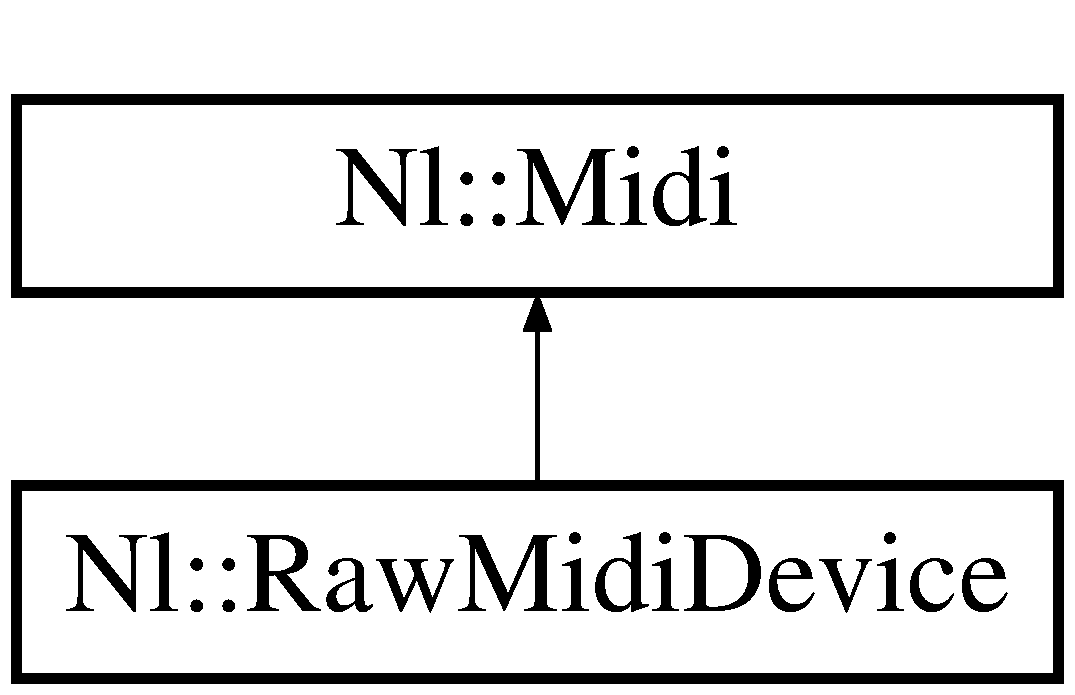
\includegraphics[height=2.000000cm]{classNl_1_1Midi}
\end{center}
\end{figure}
\subsection*{Public Member Functions}
\begin{DoxyCompactItemize}
\item 
\hypertarget{classNl_1_1Midi_add7d5ffb7a2b8cec766ee0aed15064bc}{}virtual void {\bfseries open} ()=0\label{classNl_1_1Midi_add7d5ffb7a2b8cec766ee0aed15064bc}

\item 
\hypertarget{classNl_1_1Midi_a2d831614cdfa8b799bdcf407f29210c9}{}virtual void {\bfseries close} ()=0\label{classNl_1_1Midi_a2d831614cdfa8b799bdcf407f29210c9}

\item 
\hypertarget{classNl_1_1Midi_a51f4fec3d17c920a3f5a500075c97d12}{}virtual void {\bfseries start} ()=0\label{classNl_1_1Midi_a51f4fec3d17c920a3f5a500075c97d12}

\item 
\hypertarget{classNl_1_1Midi_a4beb0e55eb868636f41777740733e5c5}{}virtual void {\bfseries stop} ()=0\label{classNl_1_1Midi_a4beb0e55eb868636f41777740733e5c5}

\end{DoxyCompactItemize}


The documentation for this class was generated from the following file\+:\begin{DoxyCompactItemize}
\item 
midi.\+h\end{DoxyCompactItemize}

\hypertarget{structNl_1_1MidiCard}{}\section{Nl\+:\+:Midi\+Card Struct Reference}
\label{structNl_1_1MidiCard}\index{Nl\+::\+Midi\+Card@{Nl\+::\+Midi\+Card}}


Definition of \hyperlink{structNl_1_1MidiCard}{Midi\+Card}.  




{\ttfamily \#include $<$rawmididevice.\+h$>$}

\subsection*{Data Fields}
\begin{DoxyCompactItemize}
\item 
\hypertarget{structNl_1_1MidiCard_a626b4accca3902d3499ddbd1c5d5172d}{}int \hyperlink{structNl_1_1MidiCard_a626b4accca3902d3499ddbd1c5d5172d}{card}\label{structNl_1_1MidiCard_a626b4accca3902d3499ddbd1c5d5172d}

\begin{DoxyCompactList}\small\item\em Alsa card number. \end{DoxyCompactList}\item 
\hypertarget{structNl_1_1MidiCard_abed00289643bf14ca00ac566a42087c9}{}std\+::list$<$ struct \hyperlink{structNl_1_1MidiDevice}{Midi\+Device} $>$ \hyperlink{structNl_1_1MidiCard_abed00289643bf14ca00ac566a42087c9}{devices}\label{structNl_1_1MidiCard_abed00289643bf14ca00ac566a42087c9}

\begin{DoxyCompactList}\small\item\em List of Midi\+Devices. \end{DoxyCompactList}\end{DoxyCompactItemize}


\subsection{Detailed Description}
Definition of \hyperlink{structNl_1_1MidiCard}{Midi\+Card}. 

The documentation for this struct was generated from the following file\+:\begin{DoxyCompactItemize}
\item 
rawmididevice.\+h\end{DoxyCompactItemize}

\hypertarget{structNl_1_1MidiDevice}{\section{Nl\-:\-:Midi\-Device Struct Reference}
\label{structNl_1_1MidiDevice}\index{Nl\-::\-Midi\-Device@{Nl\-::\-Midi\-Device}}
}


Definition of \hyperlink{structNl_1_1MidiDevice}{Midi\-Device}.  




{\ttfamily \#include $<$rawmididevice.\-h$>$}

\subsection*{Data Fields}
\begin{DoxyCompactItemize}
\item 
\hypertarget{structNl_1_1MidiDevice_a56780d796fc967d4e3b42b17c7febb13}{int \hyperlink{structNl_1_1MidiDevice_a56780d796fc967d4e3b42b17c7febb13}{device}}\label{structNl_1_1MidiDevice_a56780d796fc967d4e3b42b17c7febb13}

\begin{DoxyCompactList}\small\item\em Alsa device number. \end{DoxyCompactList}\item 
\hypertarget{structNl_1_1MidiDevice_aa6221088ffc10c61a143482da8489e12}{int \hyperlink{structNl_1_1MidiDevice_aa6221088ffc10c61a143482da8489e12}{subdevice}}\label{structNl_1_1MidiDevice_aa6221088ffc10c61a143482da8489e12}

\begin{DoxyCompactList}\small\item\em Alsa subdevice number. \end{DoxyCompactList}\item 
\hypertarget{structNl_1_1MidiDevice_ac9cd32f4346281d2d8fcf2abbbaae8b6}{Midi\-Device\-Direction \hyperlink{structNl_1_1MidiDevice_ac9cd32f4346281d2d8fcf2abbbaae8b6}{direction}}\label{structNl_1_1MidiDevice_ac9cd32f4346281d2d8fcf2abbbaae8b6}

\begin{DoxyCompactList}\small\item\em Alsa dataflow direction. \end{DoxyCompactList}\item 
\hypertarget{structNl_1_1MidiDevice_a7c697d4553518fdf5dbf9dfa9775af12}{std\-::string \hyperlink{structNl_1_1MidiDevice_a7c697d4553518fdf5dbf9dfa9775af12}{name}}\label{structNl_1_1MidiDevice_a7c697d4553518fdf5dbf9dfa9775af12}

\begin{DoxyCompactList}\small\item\em Alsa device name. \end{DoxyCompactList}\item 
\hypertarget{structNl_1_1MidiDevice_abc6e7b562234d7ca95201f18cdf837f4}{std\-::string \hyperlink{structNl_1_1MidiDevice_abc6e7b562234d7ca95201f18cdf837f4}{sub\-Name}}\label{structNl_1_1MidiDevice_abc6e7b562234d7ca95201f18cdf837f4}

\begin{DoxyCompactList}\small\item\em Alsa subdevice number. \end{DoxyCompactList}\end{DoxyCompactItemize}


\subsection{Detailed Description}
Definition of \hyperlink{structNl_1_1MidiDevice}{Midi\-Device}. 

The documentation for this struct was generated from the following file\-:\begin{DoxyCompactItemize}
\item 
rawmididevice.\-h\end{DoxyCompactItemize}

\hypertarget{classNl_1_1RawMidiDevice}{}\section{Nl\+:\+:Raw\+Midi\+Device Class Reference}
\label{classNl_1_1RawMidiDevice}\index{Nl\+::\+Raw\+Midi\+Device@{Nl\+::\+Raw\+Midi\+Device}}


\hyperlink{classNl_1_1Midi}{Midi} implementation for alsa raw midi.  




{\ttfamily \#include $<$rawmididevice.\+h$>$}

Inheritance diagram for Nl\+:\+:Raw\+Midi\+Device\+:\begin{figure}[H]
\begin{center}
\leavevmode
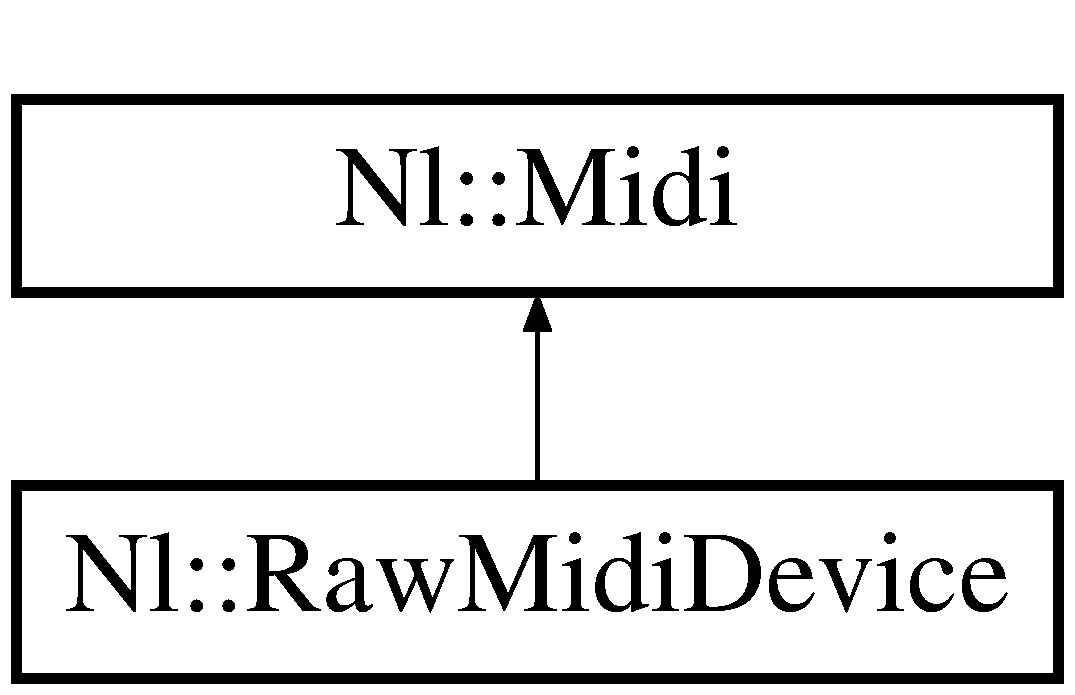
\includegraphics[height=2.000000cm]{classNl_1_1RawMidiDevice}
\end{center}
\end{figure}
\subsection*{Public Member Functions}
\begin{DoxyCompactItemize}
\item 
\hyperlink{group__Midi_ga5ad811af40ee0c2b2c97f63bd9d6163b}{Raw\+Midi\+Device} (const devicename\+\_\+t \&device, std\+::shared\+\_\+ptr$<$ \hyperlink{classNl_1_1BlockingCircularBuffer}{Blocking\+Circular\+Buffer}$<$ uint8\+\_\+t $>$$>$ buffer)
\begin{DoxyCompactList}\small\item\em Constructor. \end{DoxyCompactList}\item 
\hyperlink{group__Midi_ga8ede83b60ff88f34a597952ea1bd32fb}{$\sim$\+Raw\+Midi\+Device} ()
\begin{DoxyCompactList}\small\item\em Deconstructor. \end{DoxyCompactList}\item 
virtual void \hyperlink{group__Midi_gace91f1137effd037eca8b3b959508f91}{open} ()
\begin{DoxyCompactList}\small\item\em Open the interface. \end{DoxyCompactList}\item 
virtual void \hyperlink{group__Midi_gaa66489de15df30f282637b8a1bcd263d}{close} ()
\begin{DoxyCompactList}\small\item\em Close the interface. \end{DoxyCompactList}\item 
virtual void \hyperlink{group__Midi_ga9ca4e486b5df388d9000ea8ef48d31a8}{start} ()
\begin{DoxyCompactList}\small\item\em Start the interface. \end{DoxyCompactList}\item 
virtual void \hyperlink{group__Midi_gae95fcc2ce4b3681d34f341b2d5c9276e}{stop} ()
\begin{DoxyCompactList}\small\item\em Stop the interface. \end{DoxyCompactList}\end{DoxyCompactItemize}
\subsection*{Static Public Member Functions}
\begin{DoxyCompactItemize}
\item 
static std\+::list$<$ \hyperlink{structNl_1_1MidiCard}{Midi\+Card} $>$ \hyperlink{group__Midi_gaf6f05ac177aed9d05e06f34a776b5317}{get\+Available\+Devices} ()
\begin{DoxyCompactList}\small\item\em Static function that lists alsa midi devices. \end{DoxyCompactList}\item 
static devicename\+\_\+t \hyperlink{group__Midi_ga0b9d06ce7bef2391934e3770c4343b63}{get\+First\+Device} ()
\begin{DoxyCompactList}\small\item\em Static function that returns first available alsa midi device. \end{DoxyCompactList}\end{DoxyCompactItemize}
\subsection*{Protected Attributes}
\begin{DoxyCompactItemize}
\item 
\hypertarget{classNl_1_1RawMidiDevice_a9c773439bde734734607e1f4a39265a0}{}std\+::atomic$<$ bool $>$ {\bfseries m\+\_\+request\+Terminate}\label{classNl_1_1RawMidiDevice_a9c773439bde734734607e1f4a39265a0}

\end{DoxyCompactItemize}


\subsection{Detailed Description}
\hyperlink{classNl_1_1Midi}{Midi} implementation for alsa raw midi. 


\begin{DoxyParams}{Parameters}
{\em device} & Alsa device id such as \char`\"{}hw\+:0,1\char`\"{} \\
\hline
{\em buffer} & Buffer to store midi data to \\
\hline
\end{DoxyParams}


The documentation for this class was generated from the following files\+:\begin{DoxyCompactItemize}
\item 
rawmididevice.\+h\item 
rawmididevice.\+cpp\end{DoxyCompactItemize}

\hypertarget{classNl_1_1RawMidiDeviceException}{}\section{Nl\+:\+:Raw\+Midi\+Device\+Exception Class Reference}
\label{classNl_1_1RawMidiDeviceException}\index{Nl\+::\+Raw\+Midi\+Device\+Exception@{Nl\+::\+Raw\+Midi\+Device\+Exception}}


Definition of dataflow direction.  




{\ttfamily \#include $<$rawmididevice.\+h$>$}

Inheritance diagram for Nl\+:\+:Raw\+Midi\+Device\+Exception\+:\begin{figure}[H]
\begin{center}
\leavevmode
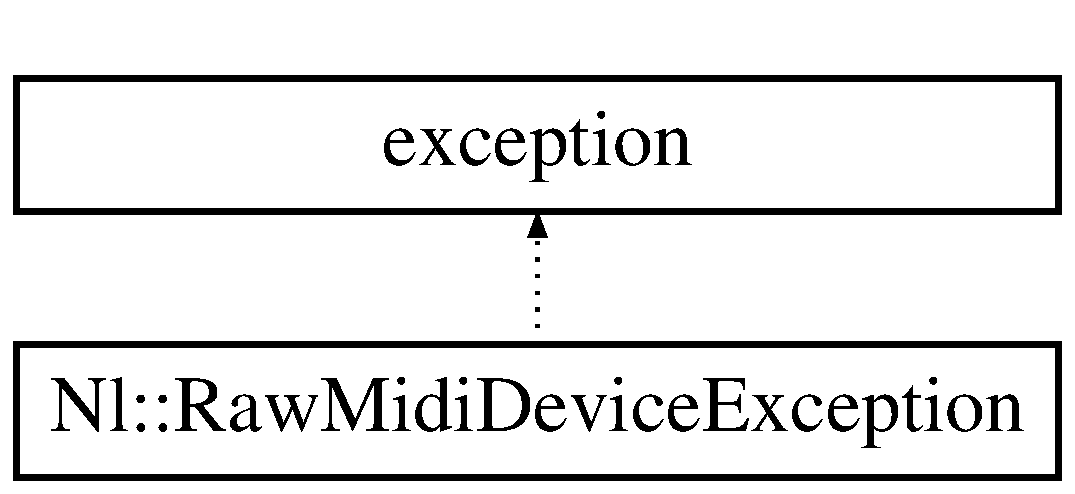
\includegraphics[height=2.000000cm]{classNl_1_1RawMidiDeviceException}
\end{center}
\end{figure}
\subsection*{Public Member Functions}
\begin{DoxyCompactItemize}
\item 
\hypertarget{classNl_1_1RawMidiDeviceException_a79b838431bf9ea9f8666684c38c036f7}{}{\bfseries Raw\+Midi\+Device\+Exception} (int error\+Number, std\+::string what)\label{classNl_1_1RawMidiDeviceException_a79b838431bf9ea9f8666684c38c036f7}

\item 
\hypertarget{classNl_1_1RawMidiDeviceException_accb4385315338ccc4ecc904fd69ab2d9}{}virtual const char $\ast$ {\bfseries what} () const noexcept\label{classNl_1_1RawMidiDeviceException_accb4385315338ccc4ecc904fd69ab2d9}

\end{DoxyCompactItemize}


\subsection{Detailed Description}
Definition of dataflow direction. 

Exception object for raw midi.


\begin{DoxyParams}{Parameters}
{\em error\+Number} & Error number given by alsa \\
\hline
{\em what} & Error description \\
\hline
\end{DoxyParams}


The documentation for this class was generated from the following file\+:\begin{DoxyCompactItemize}
\item 
rawmididevice.\+h\end{DoxyCompactItemize}

\hypertarget{structNl_1_1SampleSpecs}{\section{Nl\-:\-:Sample\-Specs Struct Reference}
\label{structNl_1_1SampleSpecs}\index{Nl\-::\-Sample\-Specs@{Nl\-::\-Sample\-Specs}}
}
\subsection*{Data Fields}
\begin{DoxyCompactItemize}
\item 
\hypertarget{structNl_1_1SampleSpecs_acb7588547dc0e783412aefe17048dedd}{unsigned int \hyperlink{structNl_1_1SampleSpecs_acb7588547dc0e783412aefe17048dedd}{samplerate}}\label{structNl_1_1SampleSpecs_acb7588547dc0e783412aefe17048dedd}

\begin{DoxyCompactList}\small\item\em Samplerate in Hz. \end{DoxyCompactList}\item 
\hypertarget{structNl_1_1SampleSpecs_a70b1a5e86b456e8cc98edc9b60a736da}{unsigned int \hyperlink{structNl_1_1SampleSpecs_a70b1a5e86b456e8cc98edc9b60a736da}{channels}}\label{structNl_1_1SampleSpecs_a70b1a5e86b456e8cc98edc9b60a736da}

\begin{DoxyCompactList}\small\item\em Channels. \end{DoxyCompactList}\item 
\hypertarget{structNl_1_1SampleSpecs_ac77e6fe1772e7732e361d6cf8b4a90b4}{unsigned int \hyperlink{structNl_1_1SampleSpecs_ac77e6fe1772e7732e361d6cf8b4a90b4}{bytes\-Per\-Sample}}\label{structNl_1_1SampleSpecs_ac77e6fe1772e7732e361d6cf8b4a90b4}

\begin{DoxyCompactList}\small\item\em How many bytes does one sample have. 24\-\_\-\-B\-E3 = 3, S16 = 2, ... \end{DoxyCompactList}\item 
\hypertarget{structNl_1_1SampleSpecs_a787b31b3cd063a0680d46e1b7029906b}{unsigned int \hyperlink{structNl_1_1SampleSpecs_a787b31b3cd063a0680d46e1b7029906b}{bytes\-Per\-Sample\-Physical}}\label{structNl_1_1SampleSpecs_a787b31b3cd063a0680d46e1b7029906b}

\begin{DoxyCompactList}\small\item\em Sometimes 24\-\_\-\-B\-E3 can be stored in 4\-Bytes, then this would be 4. Usually same as bytes\-Per\-Sample. \end{DoxyCompactList}\item 
\hypertarget{structNl_1_1SampleSpecs_af46b90202f051155b9ea1e528b0533af}{unsigned int \hyperlink{structNl_1_1SampleSpecs_af46b90202f051155b9ea1e528b0533af}{bytes\-Per\-Frame}}\label{structNl_1_1SampleSpecs_af46b90202f051155b9ea1e528b0533af}

\begin{DoxyCompactList}\small\item\em How many bytes does one frame have. Same as channels $\ast$ bytes\-Per\-Sample. \end{DoxyCompactList}\item 
\hypertarget{structNl_1_1SampleSpecs_a221d5b748fbbd0709247e6a288046fe7}{unsigned int \hyperlink{structNl_1_1SampleSpecs_a221d5b748fbbd0709247e6a288046fe7}{buffersize\-In\-Frames}}\label{structNl_1_1SampleSpecs_a221d5b748fbbd0709247e6a288046fe7}

\begin{DoxyCompactList}\small\item\em Buffersize in Frames. \end{DoxyCompactList}\item 
\hypertarget{structNl_1_1SampleSpecs_ab618cd09f45d5e7ef4af9fb74abdec5c}{unsigned int \hyperlink{structNl_1_1SampleSpecs_ab618cd09f45d5e7ef4af9fb74abdec5c}{buffersize\-In\-Frames\-Per\-Periode}}\label{structNl_1_1SampleSpecs_ab618cd09f45d5e7ef4af9fb74abdec5c}

\begin{DoxyCompactList}\small\item\em Buffersize in Frames per Periode. Same as buffersize\-In\-Frames / periodes. \end{DoxyCompactList}\item 
\hypertarget{structNl_1_1SampleSpecs_a448aeb917238293c6661824cea4d40d7}{unsigned int \hyperlink{structNl_1_1SampleSpecs_a448aeb917238293c6661824cea4d40d7}{buffersize\-In\-Bytes}}\label{structNl_1_1SampleSpecs_a448aeb917238293c6661824cea4d40d7}

\begin{DoxyCompactList}\small\item\em Buffersize in Bytes. \end{DoxyCompactList}\item 
\hypertarget{structNl_1_1SampleSpecs_a294961439505dbba77255abccf87b484}{unsigned int \hyperlink{structNl_1_1SampleSpecs_a294961439505dbba77255abccf87b484}{buffersize\-In\-Bytes\-Per\-Periode}}\label{structNl_1_1SampleSpecs_a294961439505dbba77255abccf87b484}

\begin{DoxyCompactList}\small\item\em Buffersize in Bytes per Periode. Same as buffersize\-In\-Bytes / periodes. \end{DoxyCompactList}\item 
\hypertarget{structNl_1_1SampleSpecs_a273b5caf73e4a28ca599d5c28e8773eb}{unsigned int \hyperlink{structNl_1_1SampleSpecs_a273b5caf73e4a28ca599d5c28e8773eb}{buffersize\-In\-Samples}}\label{structNl_1_1SampleSpecs_a273b5caf73e4a28ca599d5c28e8773eb}

\begin{DoxyCompactList}\small\item\em Buffersize in Samples. Same as buffersize\-In\-Bytes / bytes\-Per\-Sample. \end{DoxyCompactList}\item 
\hypertarget{structNl_1_1SampleSpecs_a0eada55de7ffd0e7e003c0e7b1178f9e}{unsigned int \hyperlink{structNl_1_1SampleSpecs_a0eada55de7ffd0e7e003c0e7b1178f9e}{buffersize\-In\-Samples\-Per\-Periode}}\label{structNl_1_1SampleSpecs_a0eada55de7ffd0e7e003c0e7b1178f9e}

\begin{DoxyCompactList}\small\item\em Buffersize in Samples per Periode. Same as buffersize\-In\-Samples / periodes. \end{DoxyCompactList}\item 
\hypertarget{structNl_1_1SampleSpecs_af8f9731e285cf005f5376f8336537802}{bool \hyperlink{structNl_1_1SampleSpecs_af8f9731e285cf005f5376f8336537802}{is\-Float}}\label{structNl_1_1SampleSpecs_af8f9731e285cf005f5376f8336537802}

\begin{DoxyCompactList}\small\item\em Are we working with floating point samples? \end{DoxyCompactList}\item 
\hypertarget{structNl_1_1SampleSpecs_afbe0390e78858f374b33be0a1bd52e63}{bool \hyperlink{structNl_1_1SampleSpecs_afbe0390e78858f374b33be0a1bd52e63}{is\-Little\-Endian}}\label{structNl_1_1SampleSpecs_afbe0390e78858f374b33be0a1bd52e63}

\begin{DoxyCompactList}\small\item\em Are we working in little endian? \end{DoxyCompactList}\item 
\hypertarget{structNl_1_1SampleSpecs_aa0438c5aab14844ec311f736024c4507}{bool \hyperlink{structNl_1_1SampleSpecs_aa0438c5aab14844ec311f736024c4507}{is\-Signed}}\label{structNl_1_1SampleSpecs_aa0438c5aab14844ec311f736024c4507}

\begin{DoxyCompactList}\small\item\em Are we using a sample format with signed values? \end{DoxyCompactList}\end{DoxyCompactItemize}


\subsection{Detailed Description}
Sampleinformation for an audio interface 

The documentation for this struct was generated from the following file\-:\begin{DoxyCompactItemize}
\item 
samplespecs.\-h\end{DoxyCompactItemize}

\hypertarget{classNl_1_1StopBlockTime}{\section{Nl\-:\-:Stop\-Block\-Time Class Reference}
\label{classNl_1_1StopBlockTime}\index{Nl\-::\-Stop\-Block\-Time@{Nl\-::\-Stop\-Block\-Time}}
}
\subsection*{Public Member Functions}
\begin{DoxyCompactItemize}
\item 
\hyperlink{group__Tools_ga33325d365bbddda3814093ca7e362474}{Stop\-Block\-Time} (\hyperlink{classNl_1_1StopWatch}{Stop\-Watch} $\ast$sw, std\-::string name)
\begin{DoxyCompactList}\small\item\em Constructor. \end{DoxyCompactList}\item 
\hyperlink{group__Tools_ga6b16ead71407ac4cc14b293e46bfbc3a}{$\sim$\-Stop\-Block\-Time} ()
\begin{DoxyCompactList}\small\item\em Destructor. \end{DoxyCompactList}\end{DoxyCompactItemize}


The documentation for this class was generated from the following files\-:\begin{DoxyCompactItemize}
\item 
stopwatch.\-h\item 
stopwatch.\-cpp\end{DoxyCompactItemize}

\hypertarget{classStopFunctionTime}{\section{Stop\-Function\-Time Class Reference}
\label{classStopFunctionTime}\index{Stop\-Function\-Time@{Stop\-Function\-Time}}
}


Helper class, that measures time duration for the time the object exists.  




{\ttfamily \#include $<$stopwatch.\-h$>$}



\subsection{Detailed Description}
Helper class, that measures time duration for the time the object exists. 

This class calls Stop\-Watch\-::start(\char`\"{}\char`\"{}) in constructor ans Stop\-Watch\-::stop() in destructor. Hence it can be used like this, to measure the total executiontime of a function\-:


\begin{DoxyCode}
StopWatch sw();

\textcolor{keywordtype}{void} anyFunction()
\{
   \hyperlink{classStopFunctionTime}{StopFunctionTime} sft(&sw, \textcolor{stringliteral}{"Valuename"}); \textcolor{comment}{// Start measuring time from here.}

   \textcolor{comment}{// Some very expensive code here}
\}
\end{DoxyCode}
 

The documentation for this class was generated from the following file\-:\begin{DoxyCompactItemize}
\item 
stopwatch.\-h\end{DoxyCompactItemize}

\hypertarget{classNl_1_1StopWatch}{\section{Nl\-:\-:Stop\-Watch Class Reference}
\label{classNl_1_1StopWatch}\index{Nl\-::\-Stop\-Watch@{Nl\-::\-Stop\-Watch}}
}


Helper class, that measures time durations.  




{\ttfamily \#include $<$stopwatch.\-h$>$}

\subsection*{Public Member Functions}
\begin{DoxyCompactItemize}
\item 
\hyperlink{group__Tools_ga086b4f40c93978f661d5154f31081677}{Stop\-Watch} (const std\-::string \&name)
\begin{DoxyCompactList}\small\item\em Constructor. \end{DoxyCompactList}\item 
void \hyperlink{group__Tools_ga0171f821750460729b49db731d20e214}{start} (const std\-::string \&name)
\begin{DoxyCompactList}\small\item\em Set start timestamp to now. \end{DoxyCompactList}\item 
void \hyperlink{group__Tools_ga2b770511bceacff939c8bbf69e25445f}{stop} ()
\begin{DoxyCompactList}\small\item\em Set stop timestamp to now. \end{DoxyCompactList}\item 
std\-::ostream \& \hyperlink{group__Tools_gacd1b3793ab5f126af64122dcfabf1020}{print\-Detailed} (std\-::ostream \&rhs)
\begin{DoxyCompactList}\small\item\em Prints a detailed list with all timestamps. \end{DoxyCompactList}\item 
std\-::ostream \& \hyperlink{group__Tools_ga8d07863904ca88de29fe3906ee1ae0a6}{print\-Summary} (std\-::ostream \&rhs)
\begin{DoxyCompactList}\small\item\em Prints a summary of all timestamps. \end{DoxyCompactList}\end{DoxyCompactItemize}


\subsection{Detailed Description}
Helper class, that measures time durations. 

This class can be used to log execution time.


\begin{DoxyCode}
\hyperlink{group__Tools_ga086b4f40c93978f661d5154f31081677}{StopWatch} sw();
\textcolor{keywordtype}{void} anyFunction()
\{
   sw.\hyperlink{group__Tools_ga0171f821750460729b49db731d20e214}{start}(\textcolor{stringliteral}{"TimePointName"});
   \textcolor{comment}{// Some very expensive code here}
   sw.\hyperlink{group__Tools_ga2b770511bceacff939c8bbf69e25445f}{stop}();
\}
\end{DoxyCode}
 

The documentation for this class was generated from the following files\-:\begin{DoxyCompactItemize}
\item 
stopwatch.\-h\item 
stopwatch.\-cpp\end{DoxyCompactItemize}

\hypertarget{structNl_1_1Timestamp}{\section{Nl\-:\-:Timestamp Struct Reference}
\label{structNl_1_1Timestamp}\index{Nl\-::\-Timestamp@{Nl\-::\-Timestamp}}
}
\subsection*{Data Fields}
\begin{DoxyCompactItemize}
\item 
\hypertarget{structNl_1_1Timestamp_a7d304f09a6d3be65abe2b9877fd4189d}{std\-::chrono\-::time\-\_\-point\\*
$<$ std\-::chrono\-::high\-\_\-resolution\-\_\-clock $>$ \hyperlink{structNl_1_1Timestamp_a7d304f09a6d3be65abe2b9877fd4189d}{start}}\label{structNl_1_1Timestamp_a7d304f09a6d3be65abe2b9877fd4189d}

\begin{DoxyCompactList}\small\item\em Start Time of the time stamp. \end{DoxyCompactList}\item 
\hypertarget{structNl_1_1Timestamp_ab45c53005c458d64af09798ffc569db8}{std\-::chrono\-::time\-\_\-point\\*
$<$ std\-::chrono\-::high\-\_\-resolution\-\_\-clock $>$ \hyperlink{structNl_1_1Timestamp_ab45c53005c458d64af09798ffc569db8}{stop}}\label{structNl_1_1Timestamp_ab45c53005c458d64af09798ffc569db8}

\begin{DoxyCompactList}\small\item\em Stop Time of the time stamp. \end{DoxyCompactList}\item 
\hypertarget{structNl_1_1Timestamp_ae7fdd155dcabcb5e00222fba0d5f1c62}{std\-::string {\bfseries name}}\label{structNl_1_1Timestamp_ae7fdd155dcabcb5e00222fba0d5f1c62}

\end{DoxyCompactItemize}


\subsection{Detailed Description}
time stamps for execution time measurements. 

The documentation for this struct was generated from the following file\-:\begin{DoxyCompactItemize}
\item 
stopwatch.\-h\end{DoxyCompactItemize}

\hypertarget{structNl_1_1WorkingThreadHandle}{\section{Nl\-:\-:Working\-Thread\-Handle Struct Reference}
\label{structNl_1_1WorkingThreadHandle}\index{Nl\-::\-Working\-Thread\-Handle@{Nl\-::\-Working\-Thread\-Handle}}
}


The \hyperlink{structNl_1_1WorkingThreadHandle}{Working\-Thread\-Handle} struct.  




{\ttfamily \#include $<$audiofactory.\-h$>$}

\subsection*{Data Fields}
\begin{DoxyCompactItemize}
\item 
Shared\-Thread\-Handle \hyperlink{structNl_1_1WorkingThreadHandle_a8f3a12233057ef18fd8a23e0fe115223}{thread}
\item 
Shared\-Terminate\-Flag \hyperlink{structNl_1_1WorkingThreadHandle_aeaff58df70b1f63bd8a01334cb11eb93}{terminate\-Request}
\end{DoxyCompactItemize}


\subsection{Detailed Description}
The \hyperlink{structNl_1_1WorkingThreadHandle}{Working\-Thread\-Handle} struct. 

A handle to a working thread, as used by the callback creators\-:
\begin{DoxyItemize}
\item \hyperlink{group__Factory_ga3ef0d21bb158983dbb7fb10025f4c7df}{Nl\-::register\-In\-Out\-Callback\-On\-Buffer()}
\item \hyperlink{group__Factory_gaed5af7fdb6d3ff5d85b1f7dcdf72cb39}{Nl\-::register\-Output\-Callback\-On\-Buffer()}
\item \hyperlink{group__Factory_ga6cf9a9665bab65d08ad772de912c0012}{Nl\-::register\-Input\-Callback\-On\-Buffer()} 
\end{DoxyItemize}

\subsection{Field Documentation}
\hypertarget{structNl_1_1WorkingThreadHandle_aeaff58df70b1f63bd8a01334cb11eb93}{\index{Nl\-::\-Working\-Thread\-Handle@{Nl\-::\-Working\-Thread\-Handle}!terminate\-Request@{terminate\-Request}}
\index{terminate\-Request@{terminate\-Request}!Nl::WorkingThreadHandle@{Nl\-::\-Working\-Thread\-Handle}}
\subsubsection[{terminate\-Request}]{\setlength{\rightskip}{0pt plus 5cm}Shared\-Terminate\-Flag Nl\-::\-Working\-Thread\-Handle\-::terminate\-Request}}\label{structNl_1_1WorkingThreadHandle_aeaff58df70b1f63bd8a01334cb11eb93}
A terminate request handle \hypertarget{structNl_1_1WorkingThreadHandle_a8f3a12233057ef18fd8a23e0fe115223}{\index{Nl\-::\-Working\-Thread\-Handle@{Nl\-::\-Working\-Thread\-Handle}!thread@{thread}}
\index{thread@{thread}!Nl::WorkingThreadHandle@{Nl\-::\-Working\-Thread\-Handle}}
\subsubsection[{thread}]{\setlength{\rightskip}{0pt plus 5cm}Shared\-Thread\-Handle Nl\-::\-Working\-Thread\-Handle\-::thread}}\label{structNl_1_1WorkingThreadHandle_a8f3a12233057ef18fd8a23e0fe115223}
A thread handle 

The documentation for this struct was generated from the following file\-:\begin{DoxyCompactItemize}
\item 
audiofactory.\-h\end{DoxyCompactItemize}

%--- End generated contents ---

% Index
\newpage
\phantomsection
\addcontentsline{toc}{chapter}{Index}
\printindex

\end{document}
